%%%%%%%%%%%%%%%%%%%%%%%%%%%%%%%%%%%%%%%%%%%%%%%%%%%%%%%%%%%%%%%%%%%%%%%%%%%%%%%%%%%%%%%%%%%%%%%%%%%%%%%%%%%%%%%%%%%%%%%%%%%%%%%%%%%%%%%%%%%%%%%%%%%%%%%%%%%%%%%%%%%%%%%
%%%%%%%%%%%%%%%%%%%%%%%%%%%%%%%%%%%%%%%%%%%%%%%%%%%%%%%%%%%%%%%%%%%%%%%%%%%%%%%%%%%%%%%%%%%%%%%%%%%%%%%%%%%%%%%%%%%%%%%%%%%%%%%%%%%%%%%%%%%%%%%%%%%%%%%%%%%%%%%%%%%%%%%
\chapter{Measurement of the jet transverse momentum resolution}
\section{Pileup reweighting}
\label{res:app:pileup}

\begin{figure}[ht]
 \centering
    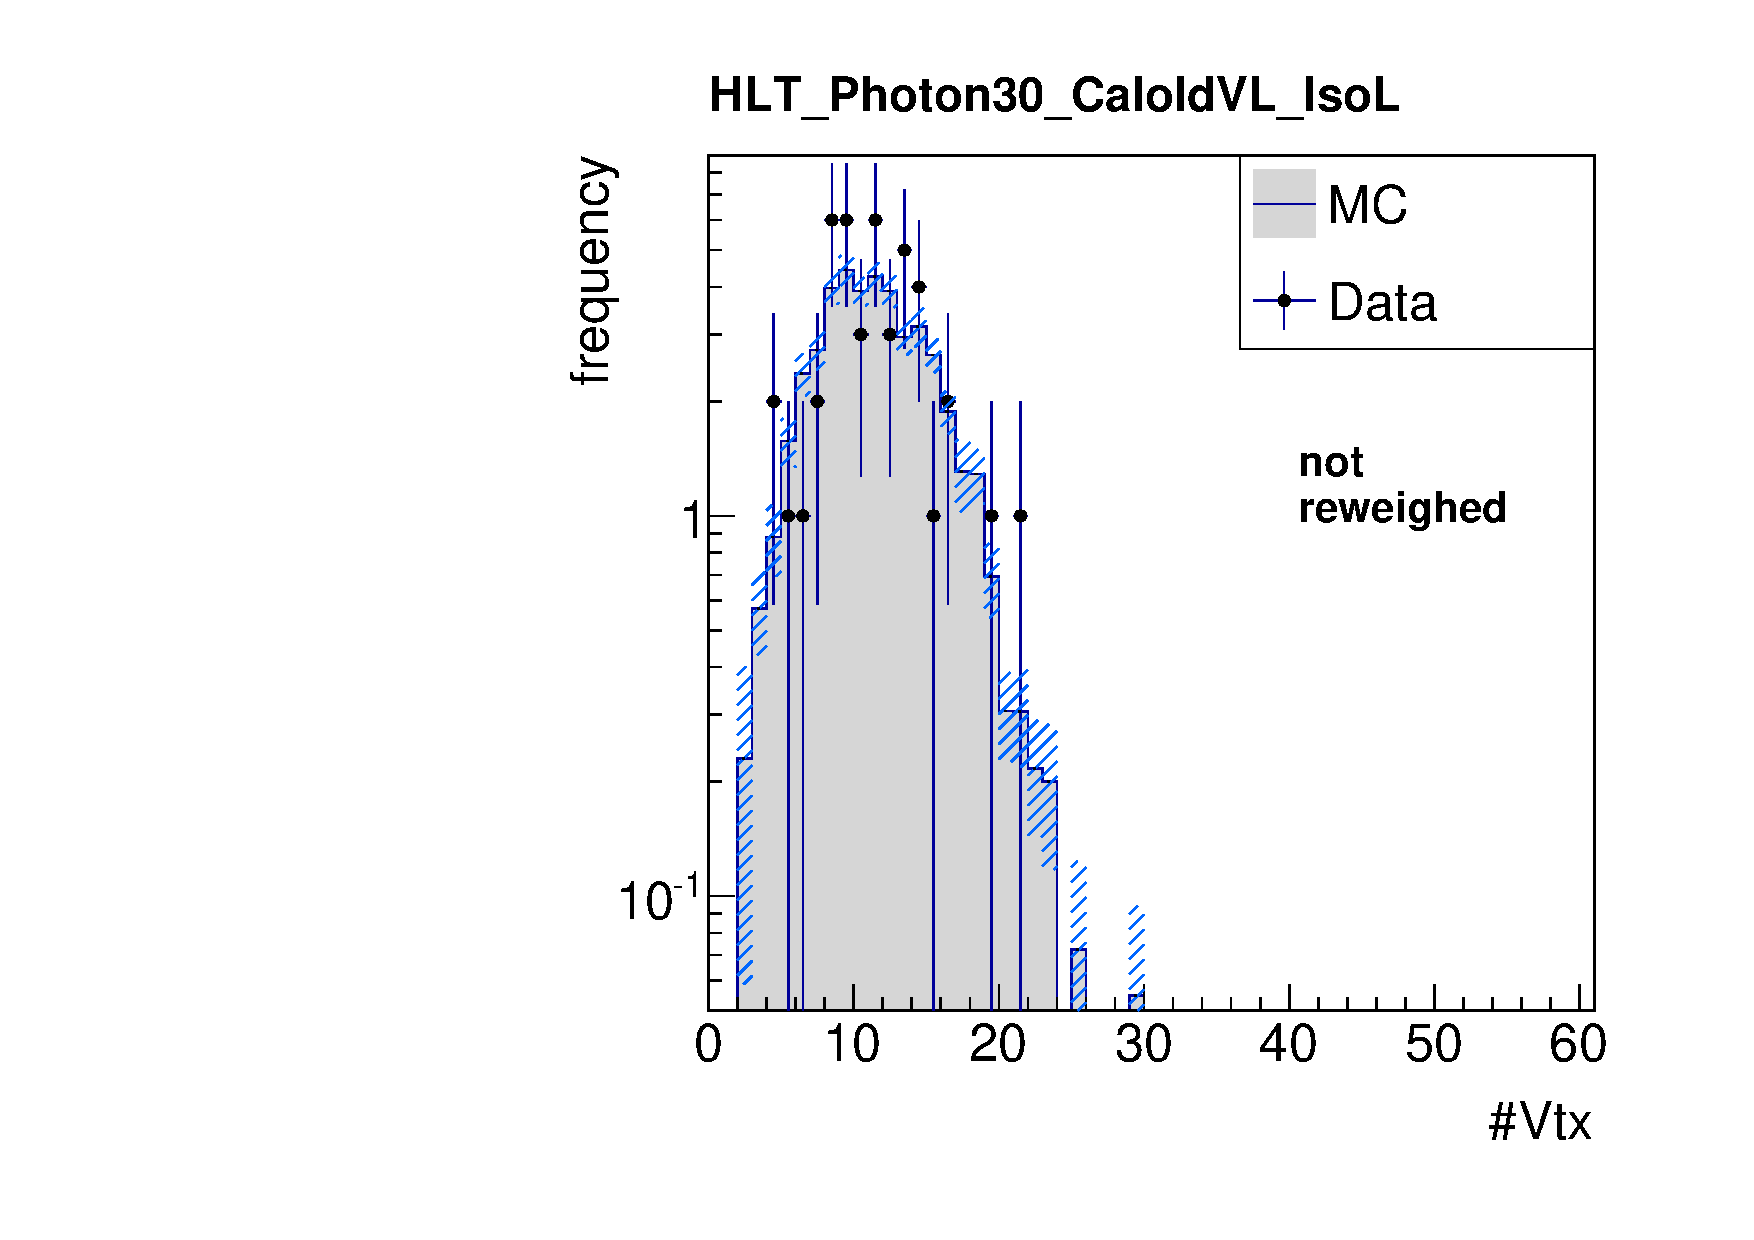
\includegraphics[width=0.22\textwidth]{figures/resolution/eventSelection/NVtxComparisonWoWeights1.pdf}
    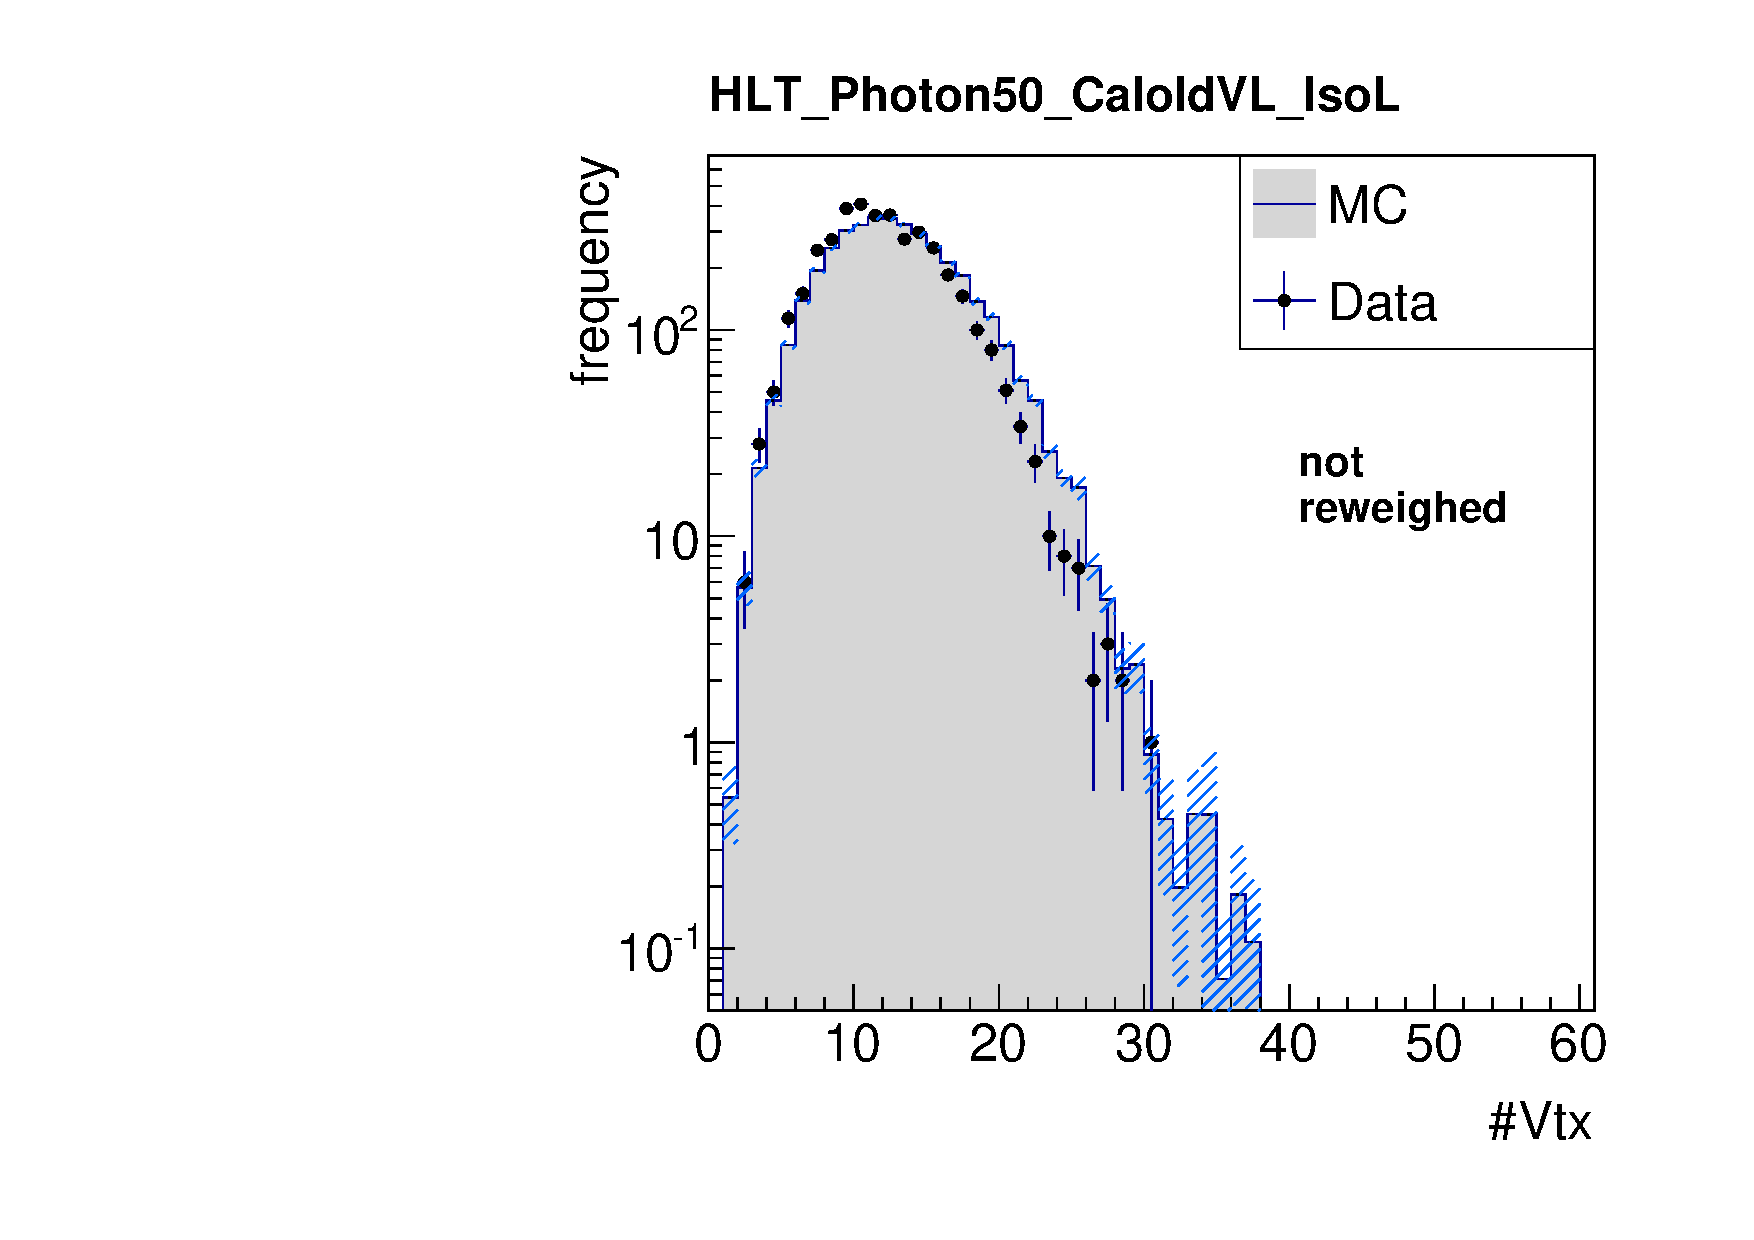
\includegraphics[width=0.22\textwidth]{figures/resolution/eventSelection/NVtxComparisonWoWeights2.pdf}
    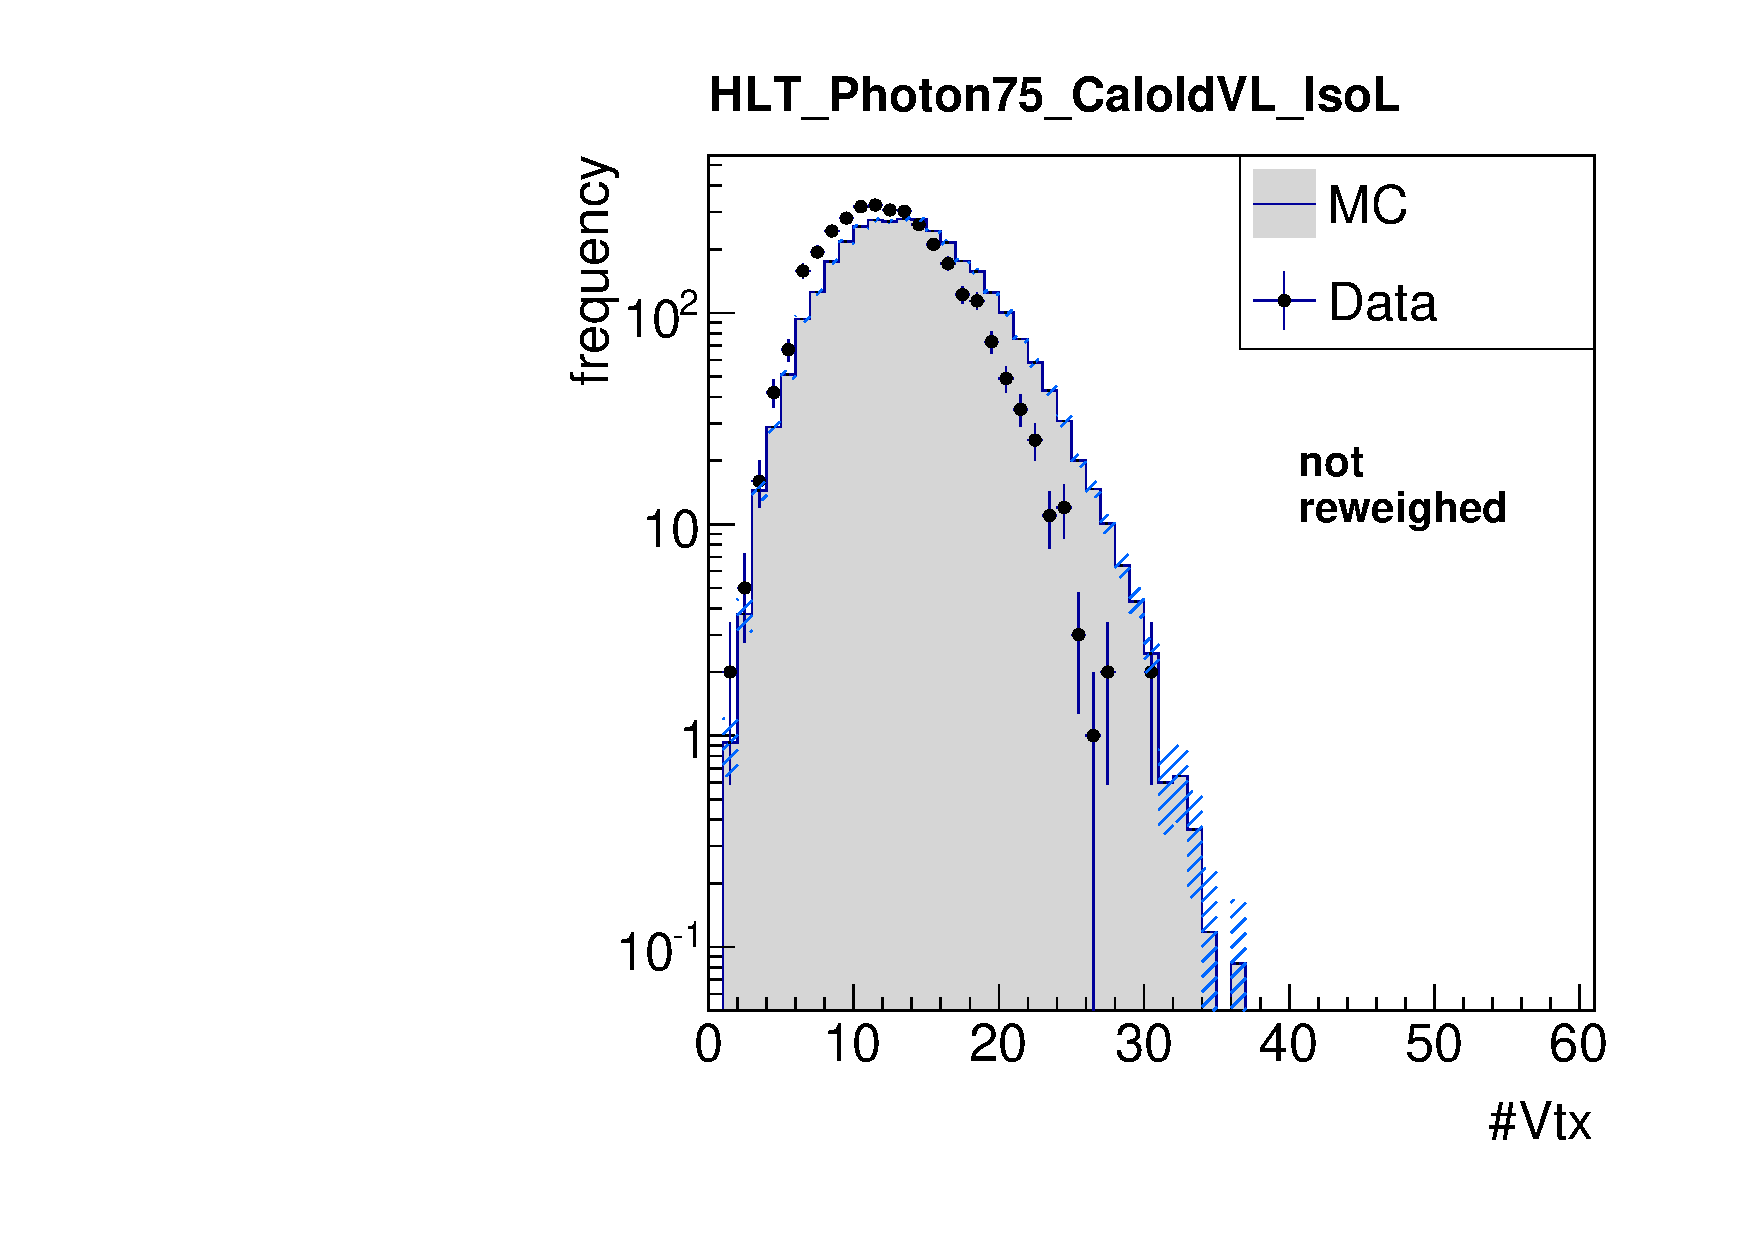
\includegraphics[width=0.22\textwidth]{figures/resolution/eventSelection/NVtxComparisonWoWeights3.pdf}

    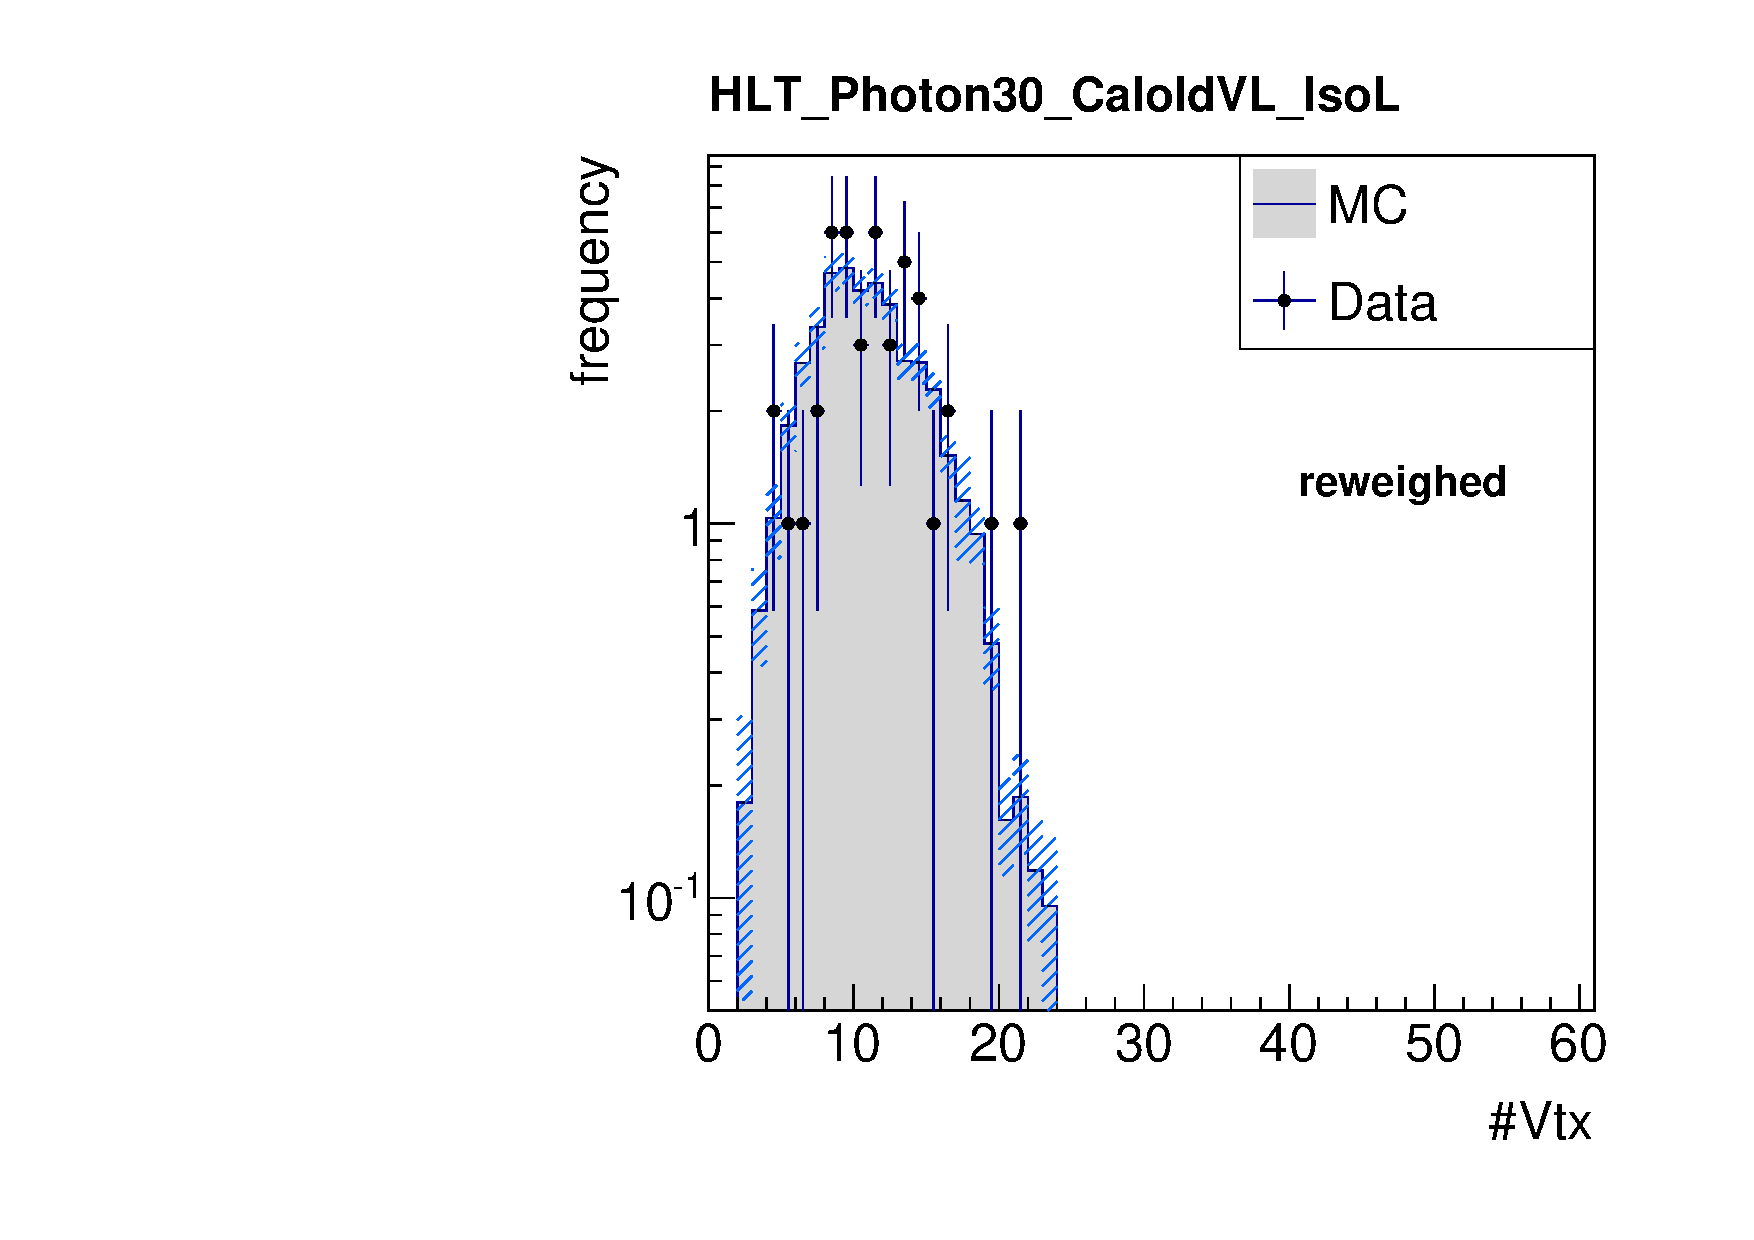
\includegraphics[width=0.22\textwidth]{figures/resolution/eventSelection/NVtxComparison1.pdf}
    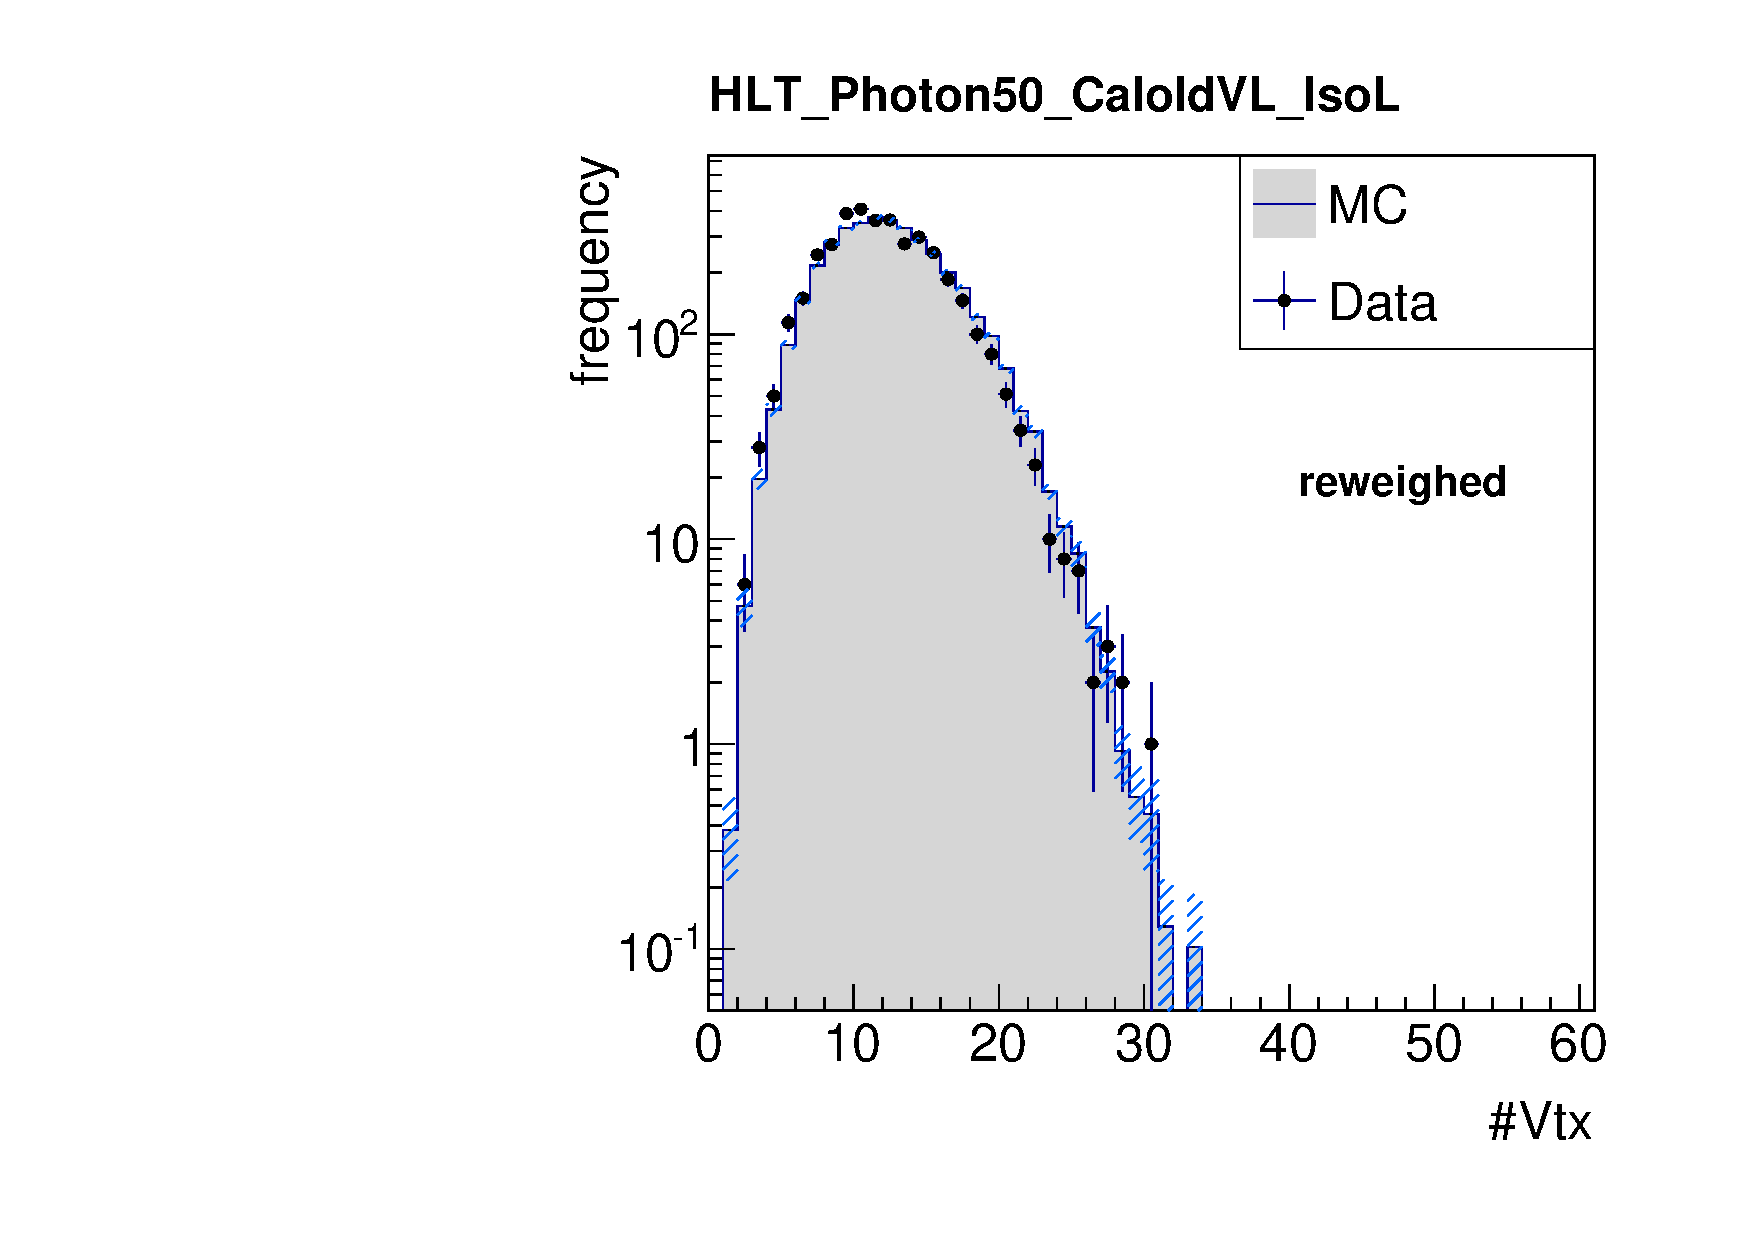
\includegraphics[width=0.22\textwidth]{figures/resolution/eventSelection/NVtxComparison2.pdf}
    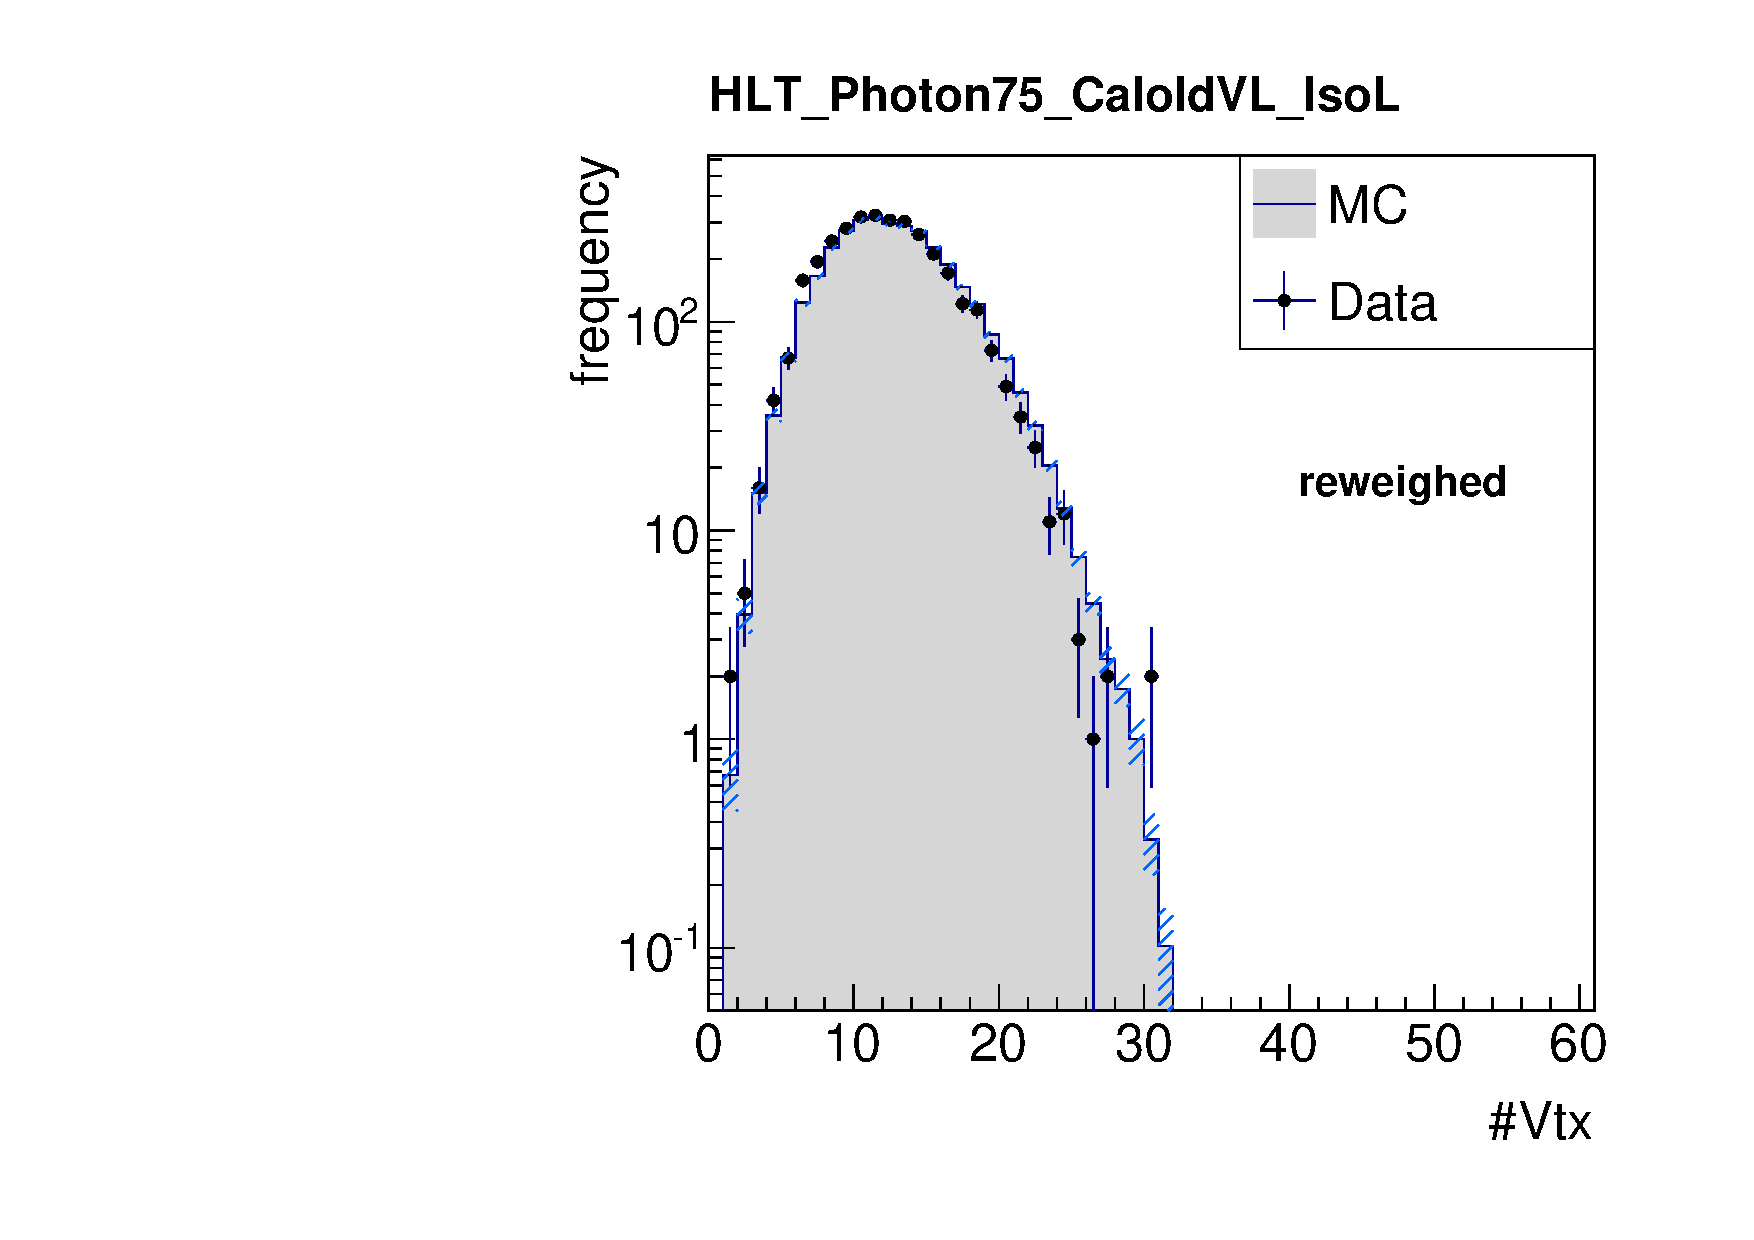
\includegraphics[width=0.22\textwidth]{figures/resolution/eventSelection/NVtxComparison3.pdf}

    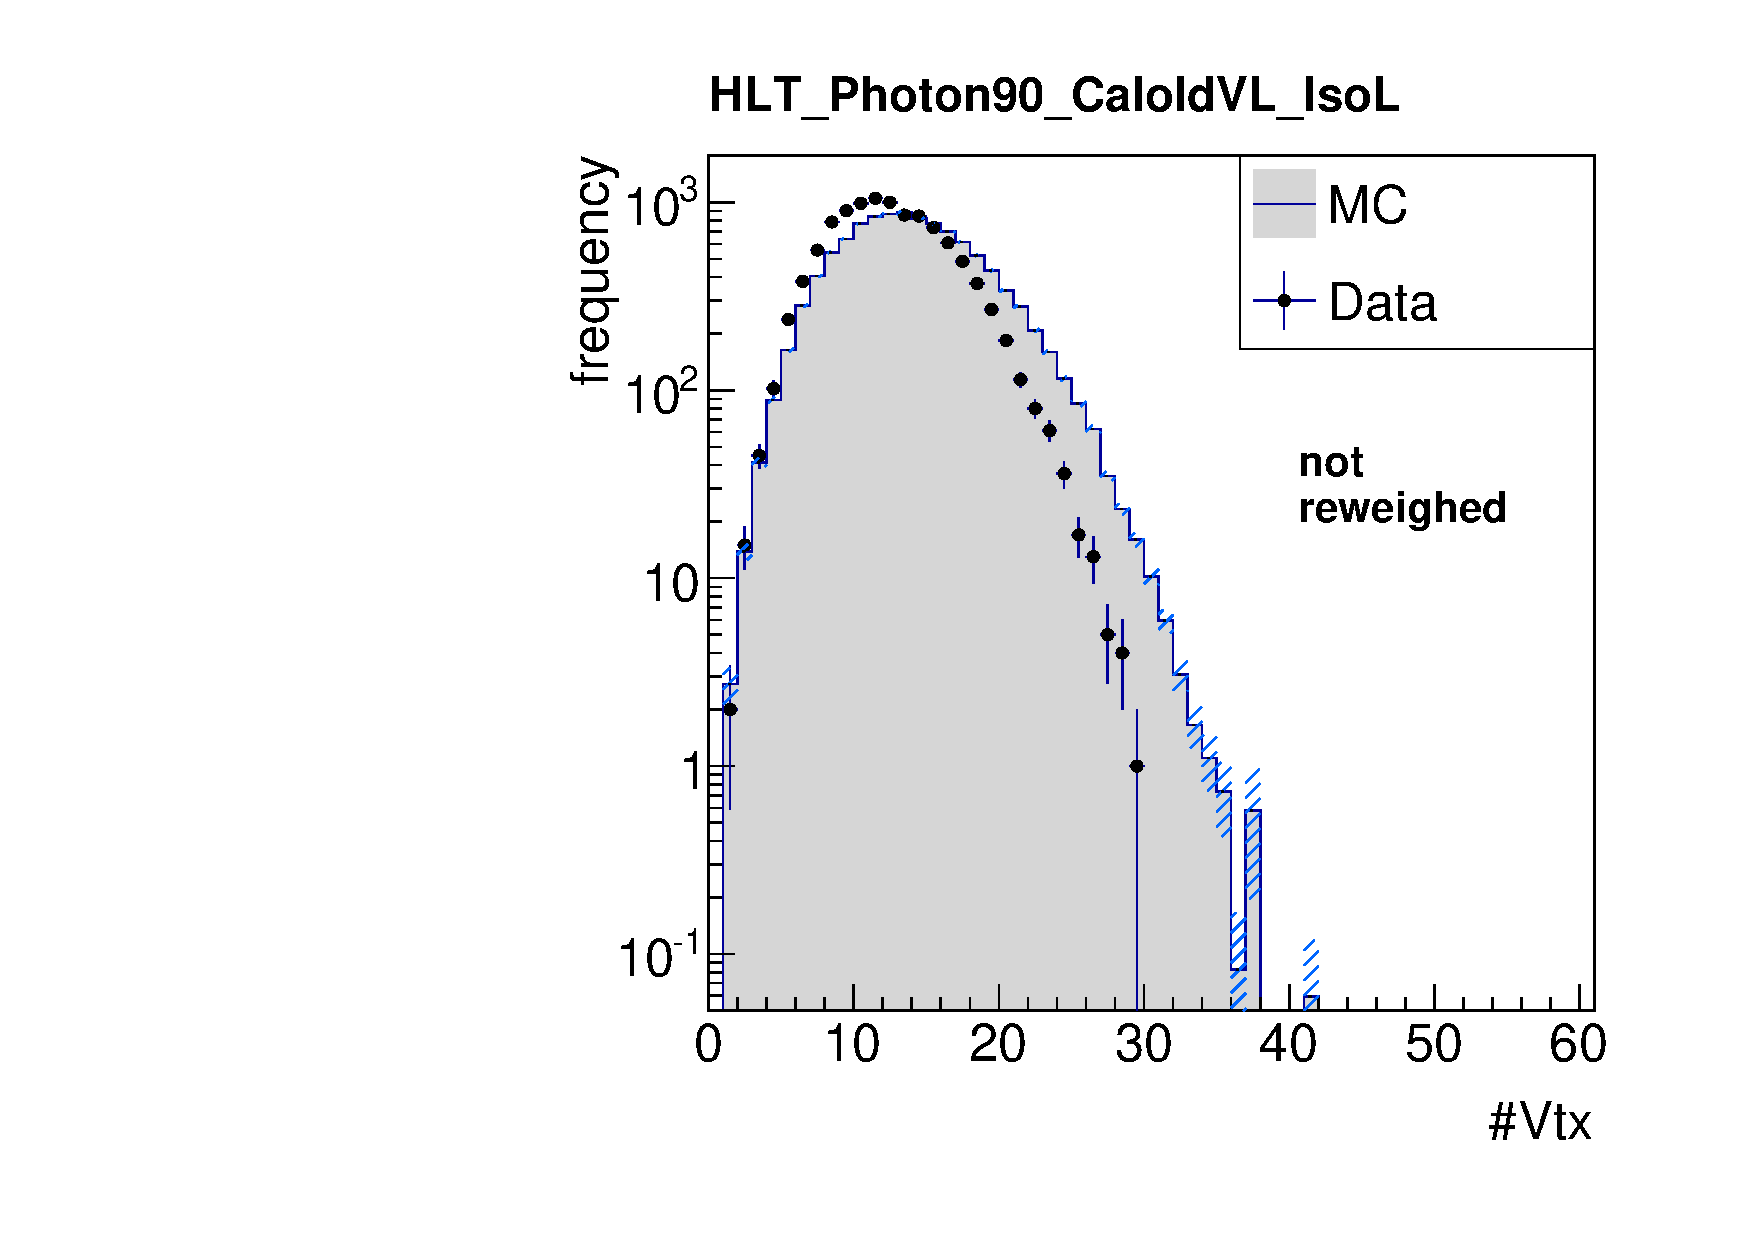
\includegraphics[width=0.22\textwidth]{figures/resolution/eventSelection/NVtxComparisonWoWeights4.pdf}
    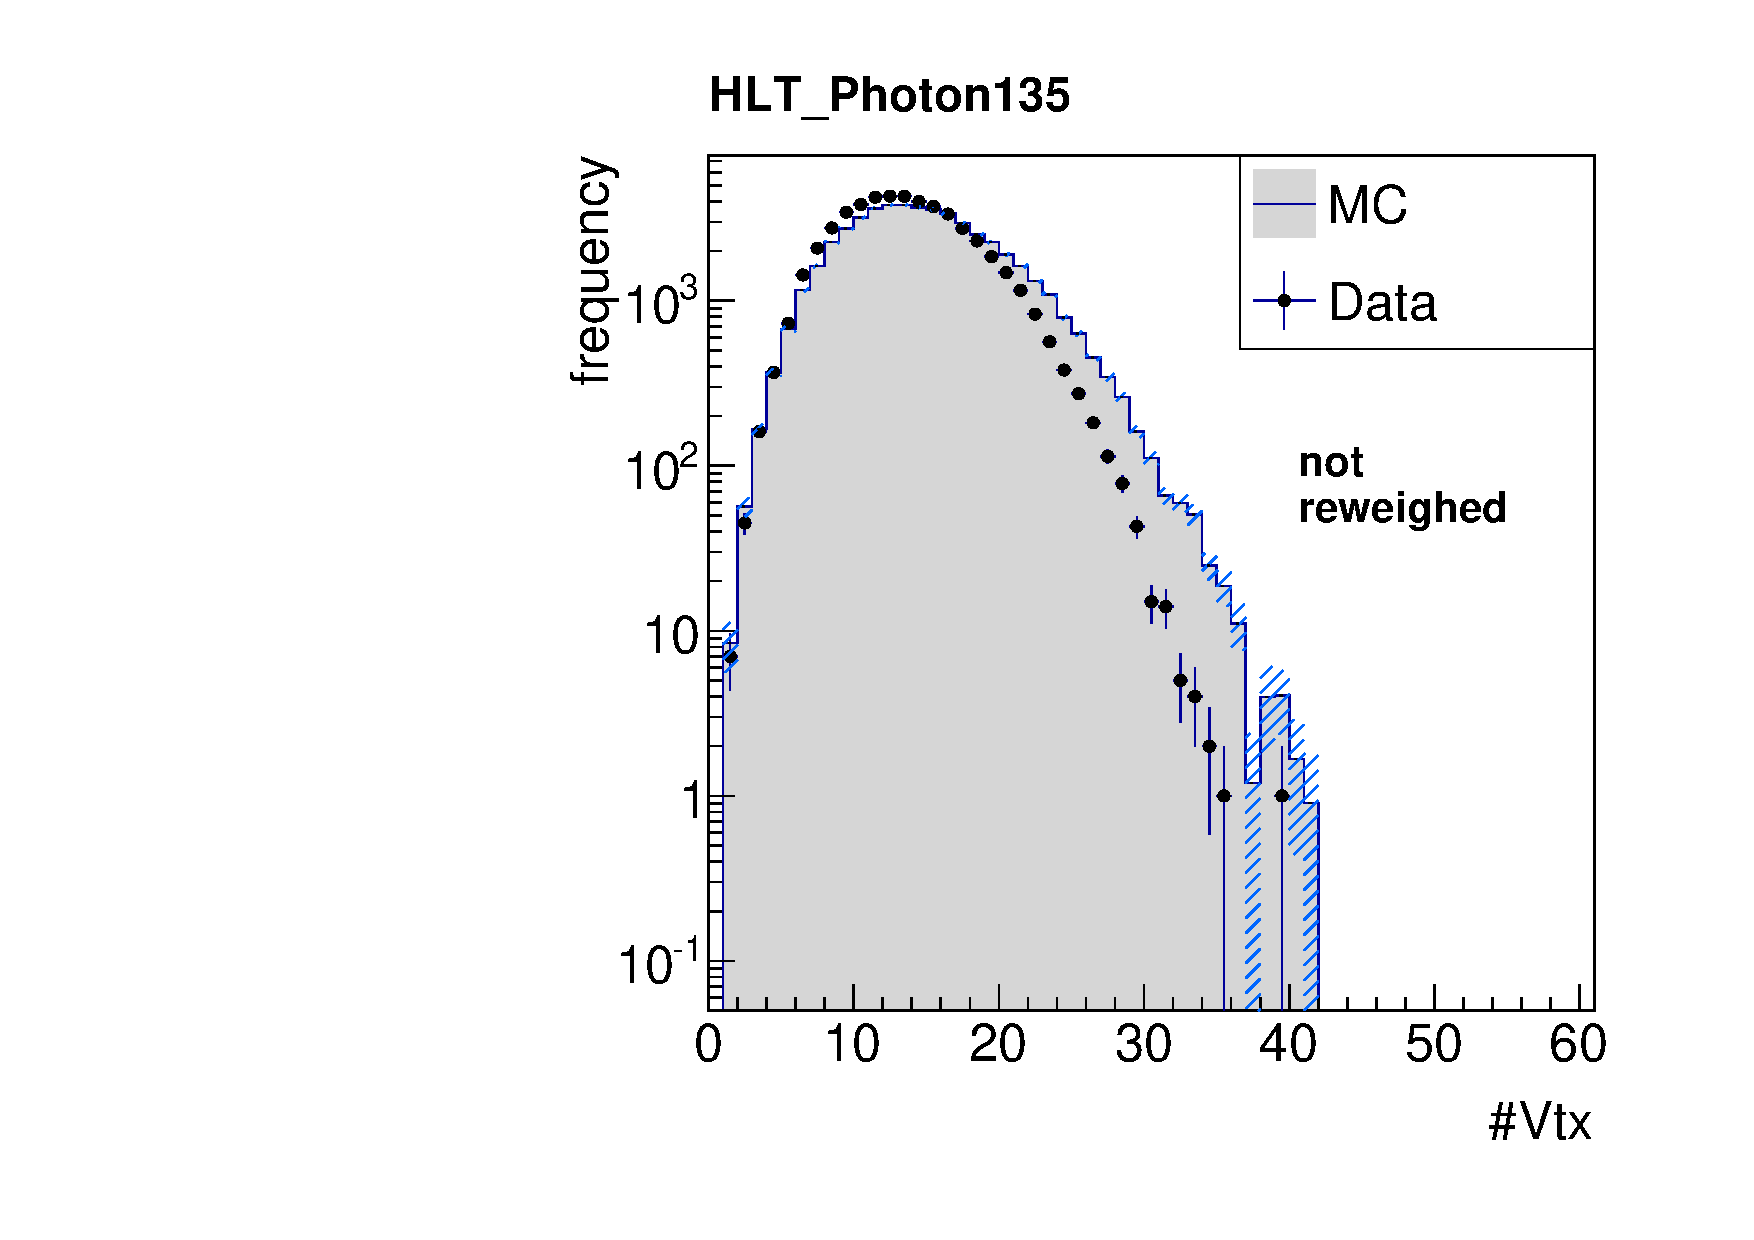
\includegraphics[width=0.22\textwidth]{figures/resolution/eventSelection/NVtxComparisonWoWeights5.pdf}
    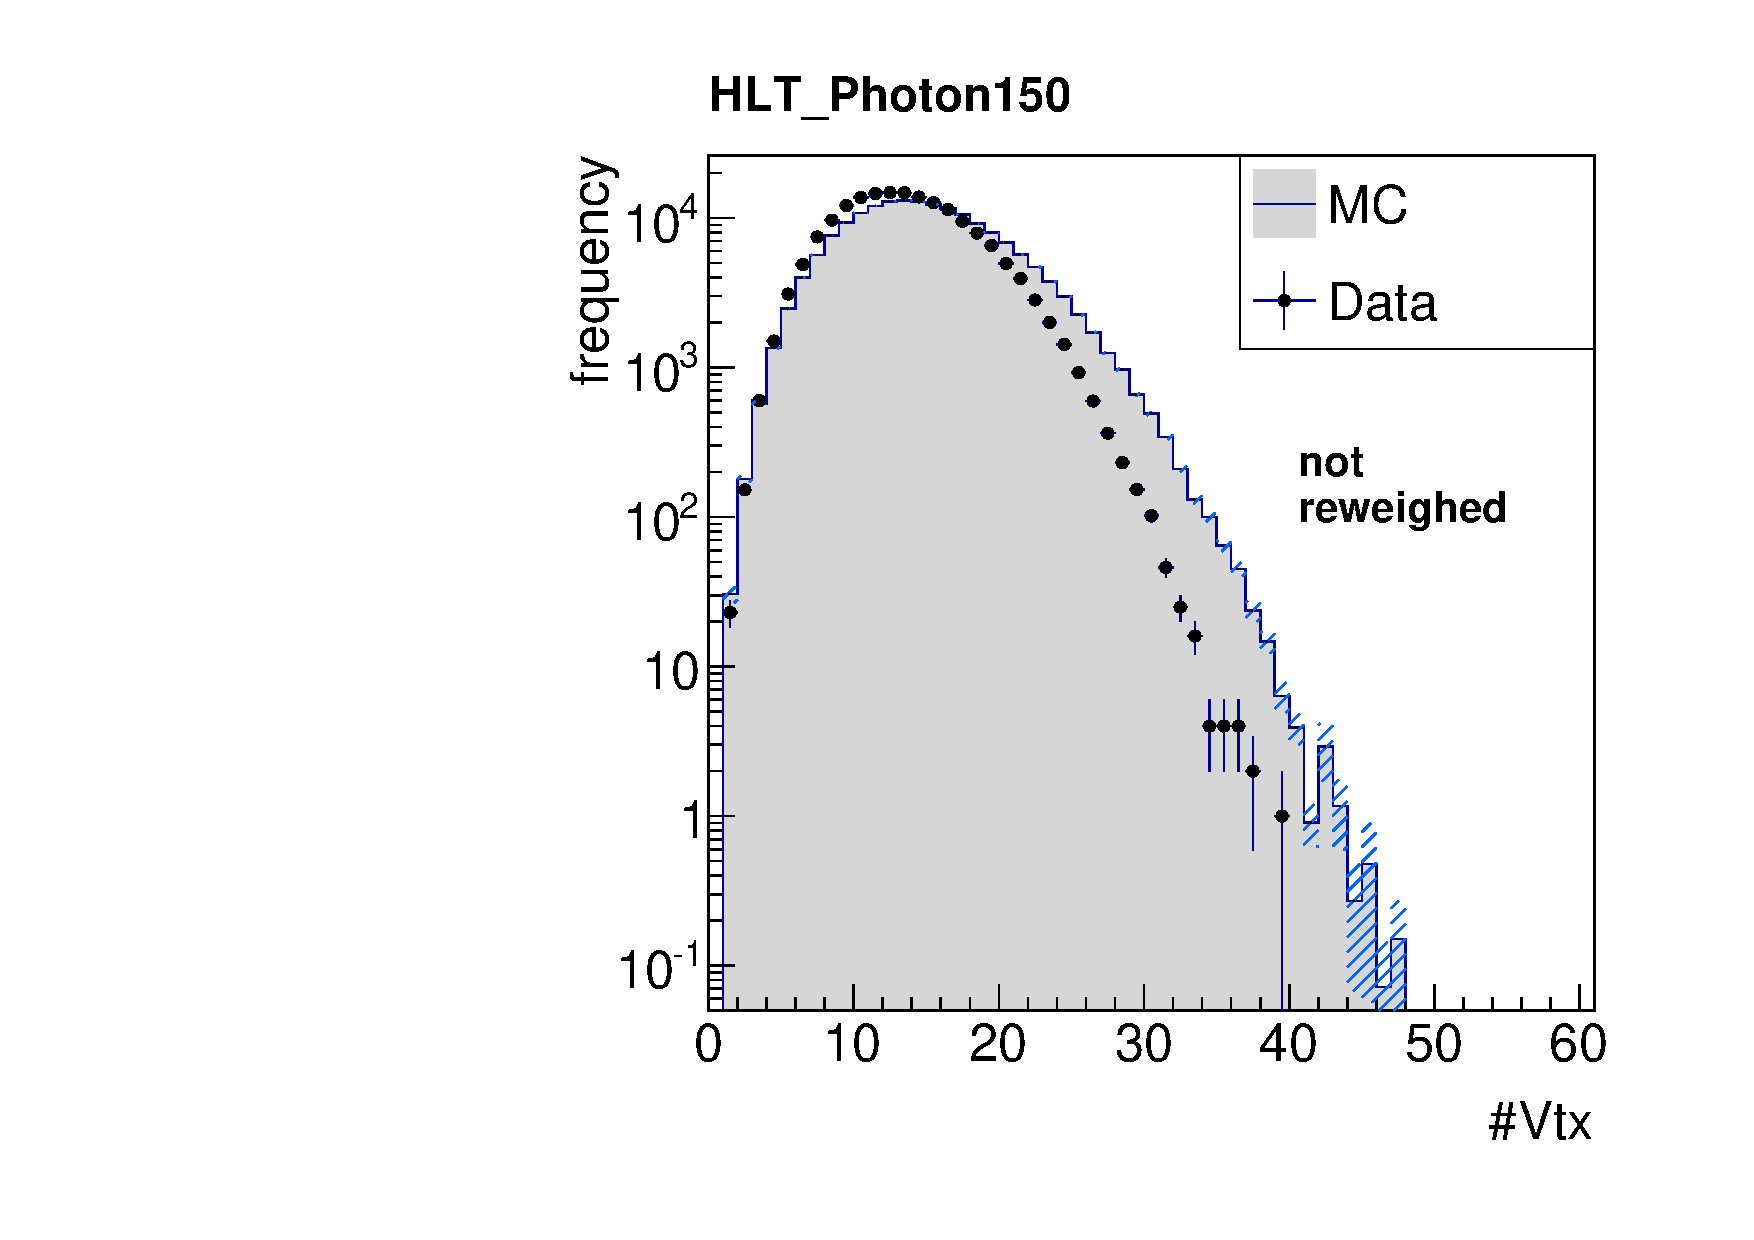
\includegraphics[width=0.22\textwidth]{figures/resolution/eventSelection/NVtxComparisonWoWeights6.pdf}

    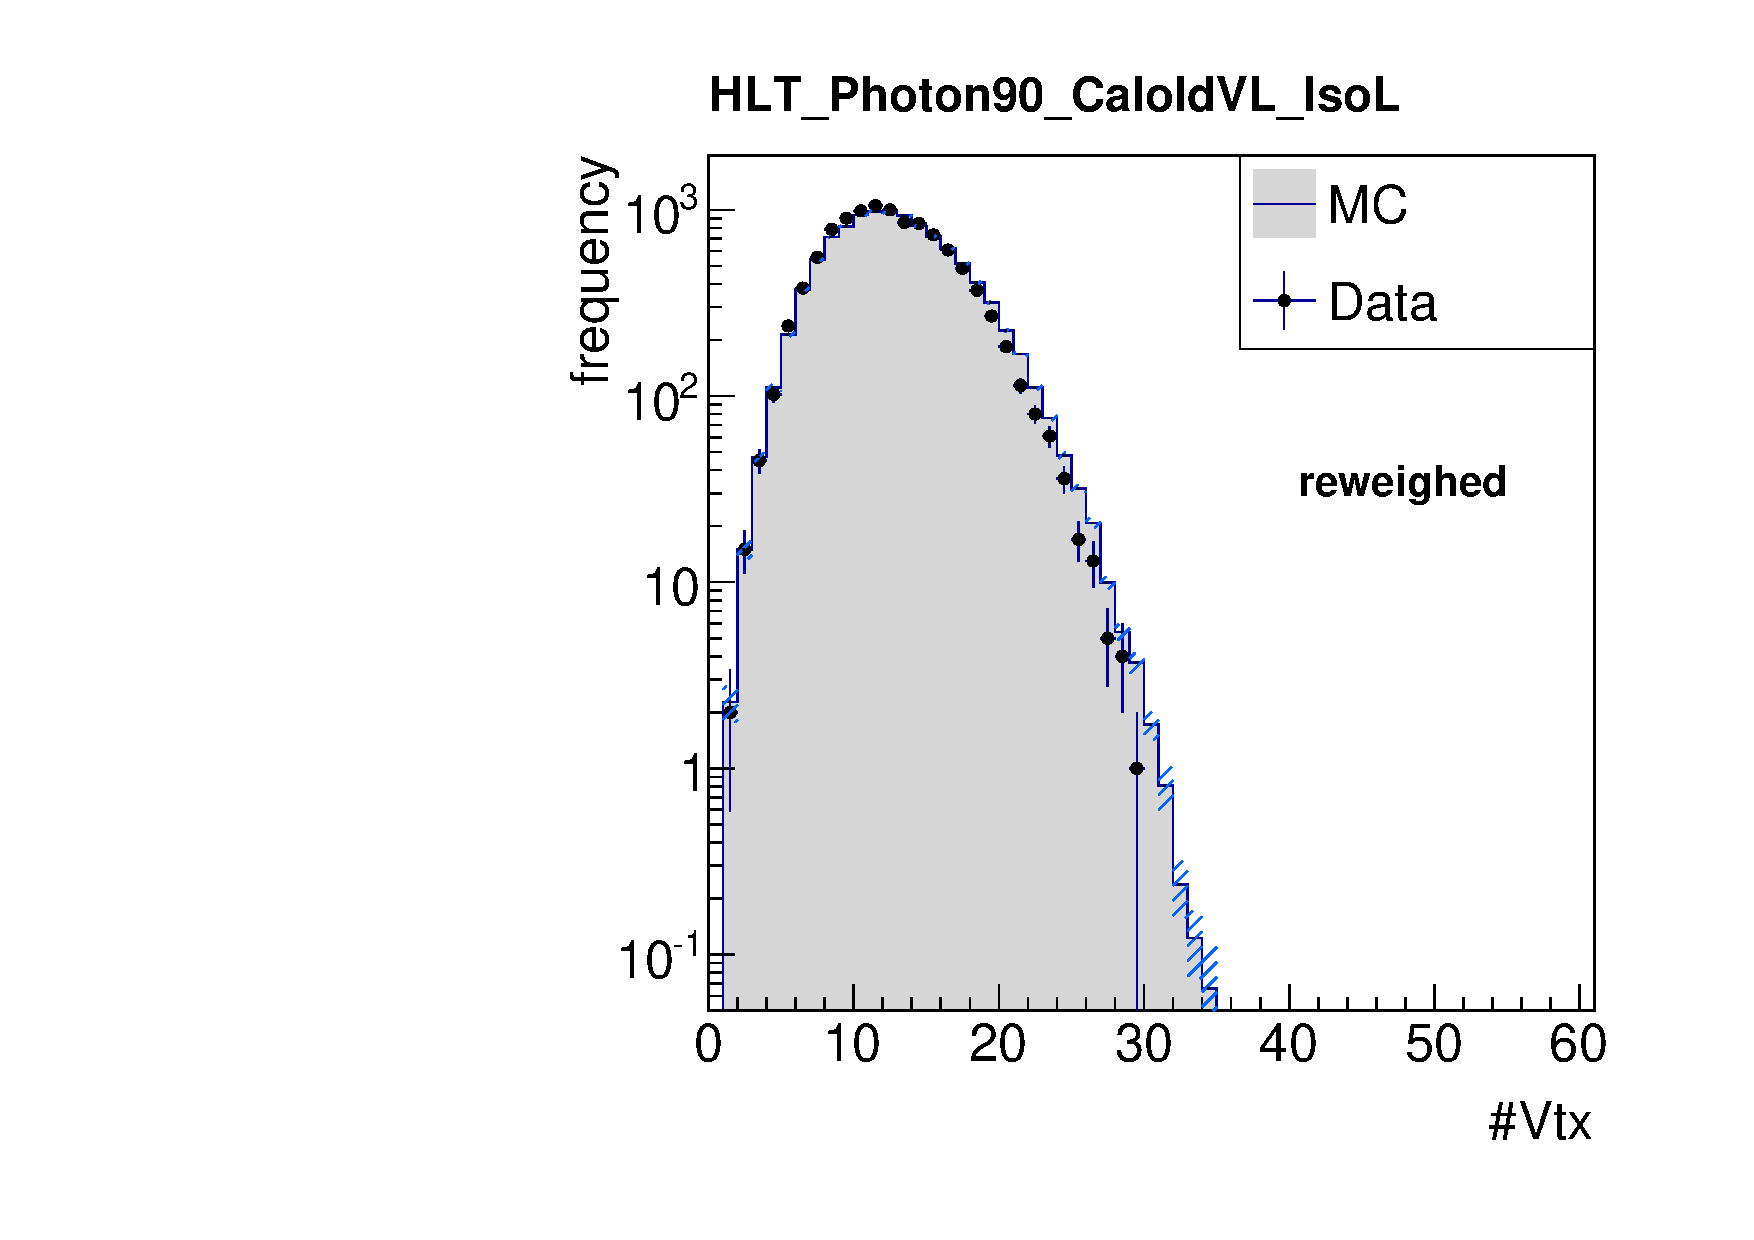
\includegraphics[width=0.22\textwidth]{figures/resolution/eventSelection/NVtxComparison4.pdf}
    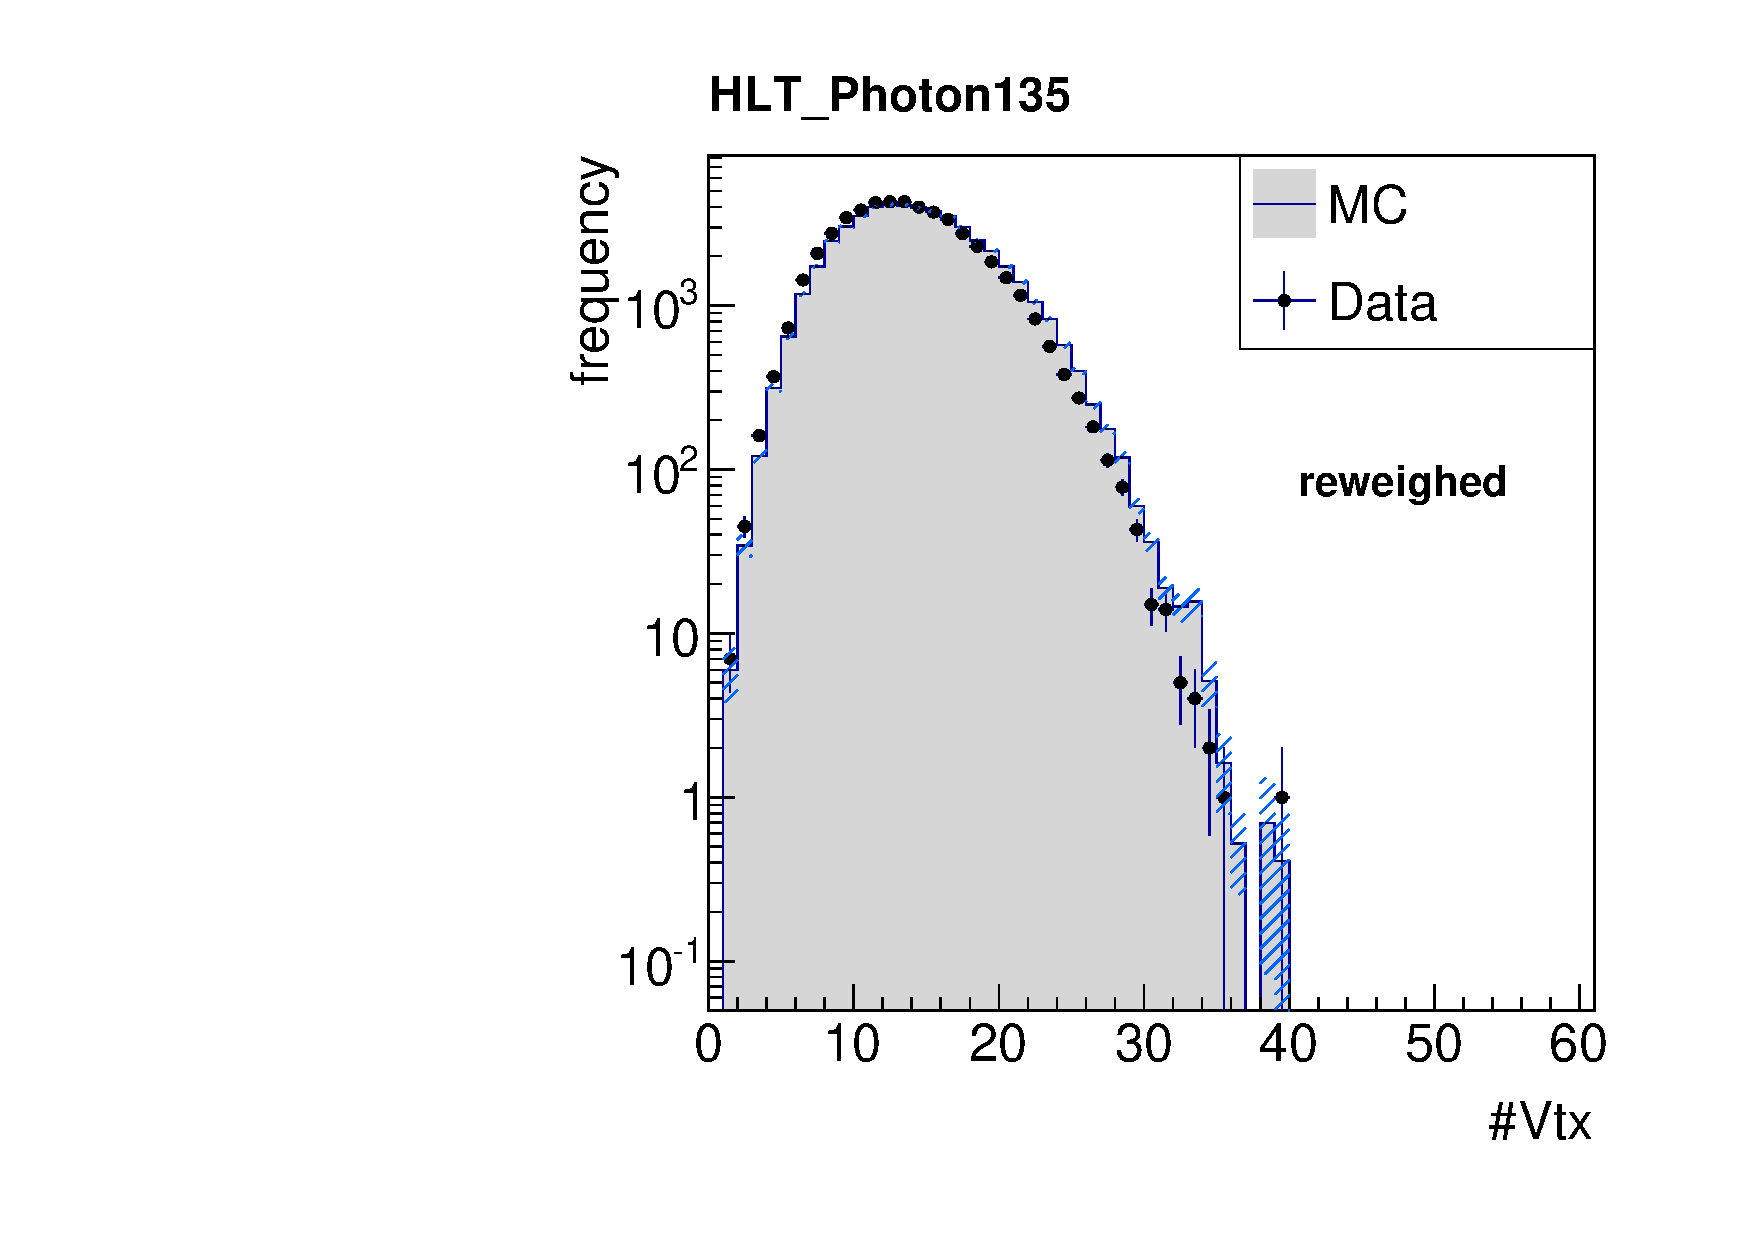
\includegraphics[width=0.22\textwidth]{figures/resolution/eventSelection/NVtxComparison5.pdf}
    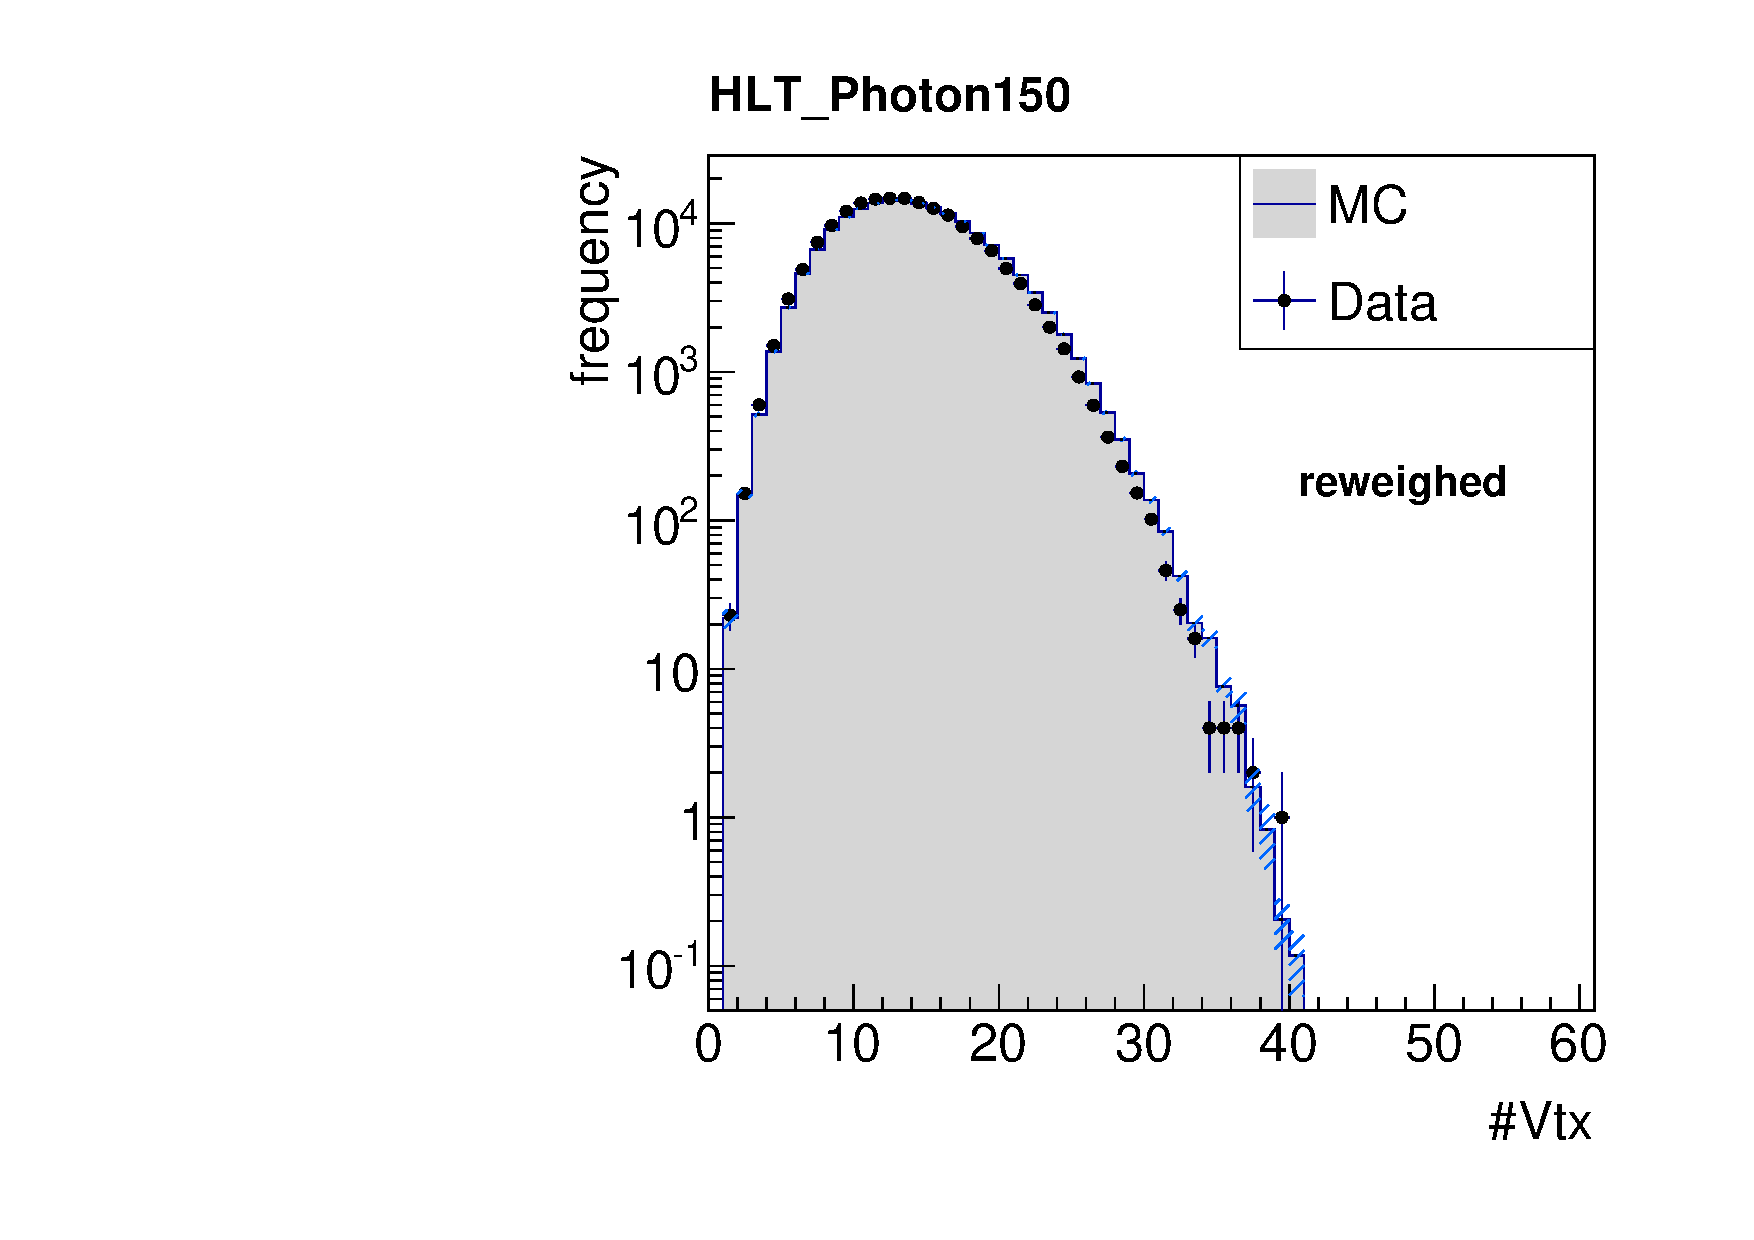
\includegraphics[width=0.22\textwidth]{figures/resolution/eventSelection/NVtxComparison6.pdf}
   \caption{The number of primary vertices in data and simulation before (1st row) and after (2nd row) pileup reweighting for $36\gev < \pt^{\gamma} < 60\gev$ (left), $60\gev < \pt^{\gamma} < 88\gev$ (middle), 
            and $88\gev < \pt^{\gamma} < 105\gev$ (right) and the number of primary vertices in data and simulation before (3rd row) and after (4th row) pileup reweighting for $105\gev < \pt^{\gamma} < 149\gev$ (left), 
            $149\gev < \pt^{\gamma} < 165\gev$ (middle), and $165\gev < \pt^{\gamma}$ (right).}
  \label{res:fig:PUreweighting}
\end{figure}

%%%%%%%%%%%%%%%%%%%%%%%%%%%%%%%%%%%%%%%%%%%%%%%%%%%%%%%%%%%%%%%%%%%%%%%%%%%%%%%%%%%%%%%%%%%%%%%%%%%%%%%%%%%%%%%%%%%%%%%%%%%%%%%%%%%%%%%%%%%%%%%%%%%%%%%%%%%%%%%%%%%%%%%
\section{Summary of all selection requirements}
\label{res:app:eventselection}


\renewcommand{\arraystretch}{1.5}
\begin{table}[!h]
\centering
\caption{Summary of all  selection criteria for the measurments of the jet transverse-momentum resolution with \GAMJET events.}
\label{res:tab:FullSelection}
\makebox[0.99\textwidth]{
\begin{tabular}{l|l}
\multicolumn{2}{c}{} \\
\toprule
One jet with                          & $\pt>10\gev$ \\
                                      & Neutral hadron fraction $<$ 0.90\\
                                      & Neutral electromagnetic fraction $<$ 0.90 \\
                                      & Number of constituents $>$ 1  \\
                                      & Charged hadron fraction $>$ 0 \\
                                      & Charged hadron multiplicity $>$ 0   \\
\midrule
One photon with                       & $\pt>22\gev$ \\
                                      & $|\eta|<1.3$ \\
                                      & $\frac{\text{H}}{\text{E}}< 0.05$ \\
                                      & $\sigma_{i\eta i \eta} < 0.013$  \\
                                      & ECAL isolation $<4.2\gev + 0.0060 \cdot \pt^{\gamma}$ \\
                                      & HCAL isolation $<2.2\gev + 0.0025 \cdot \pt^{\gamma}$  \\
                                      & Track Isolation $<2.0\gev + 0.0010 \cdot \pt^{\gamma}$ \\
                                      & Pixel seed veto  \\
\midrule
Event-based selection                 & $\pt^{\text{2nd jet}} > 10\gev$ \\
                                      & $\frac{\ptsecondjet}{\ptgamma} < 0.20$  \\
                                      & $\Delta \Phi \left(\text{\nth{1}\,jet},\, \gamma \right) > 2.95 $  \\
\bottomrule
\multicolumn{2}{c}{} \\
\end{tabular}}
\end{table}


%%%%%%%%%%%%%%%%%%%%%%%%%%%%%%%%%%%%%%%%%%%%%%%%%%%%%%%%%%%%%%%%%%%%%%%%%%%%%%%%%%%%%%%%%%%%%%%%%%%%%%%%%%%%%%%%%%%%%%%%%%%%%%%%%%%%%%%%%%%%%%%%%%%%%%%%%%%%%%%%%%%%%%%
\section{Generator-level jet flavor definition}
\label{res:app:FlavorDefinition}

The algorithmic flavor definition uses the following discrimination:

\begin{itemize}
\item Try to find the parton that most likely determines the properties of the jet and assign that flavor as true flavor
\item Here, the ``final state'' partons (after showering, radiation) are analyzed (also within $\Delta$R $<$ 0.3 of reconstructed jet cone)
\item Jets from radiation are matched with full efficiency
\item If there is a b/c within the jet cone: label as b/c
\item Otherwise: assign flavor of the hardest parton 
\end{itemize}

 
%%%%%%%%%%%%%%%%%%%%%%%%%%%%%%%%%%%%%%%%%%%%%%%%%%%%%%%%%%%%%%%%%%%%%%%%%%%%%%%%%%%%%%%%%%%%%%%%%%%%%%%%%%%%%%%%%%%%%%%%%%%%%%%%%%%%%%%%%%%%%%%%%%%%%%%%%%%%%%%%%%%%%%%
\section{Extrapolation plots}
\label{res:app:extrapolationPlots}
\begin{figure*}[ht]
 \centering
    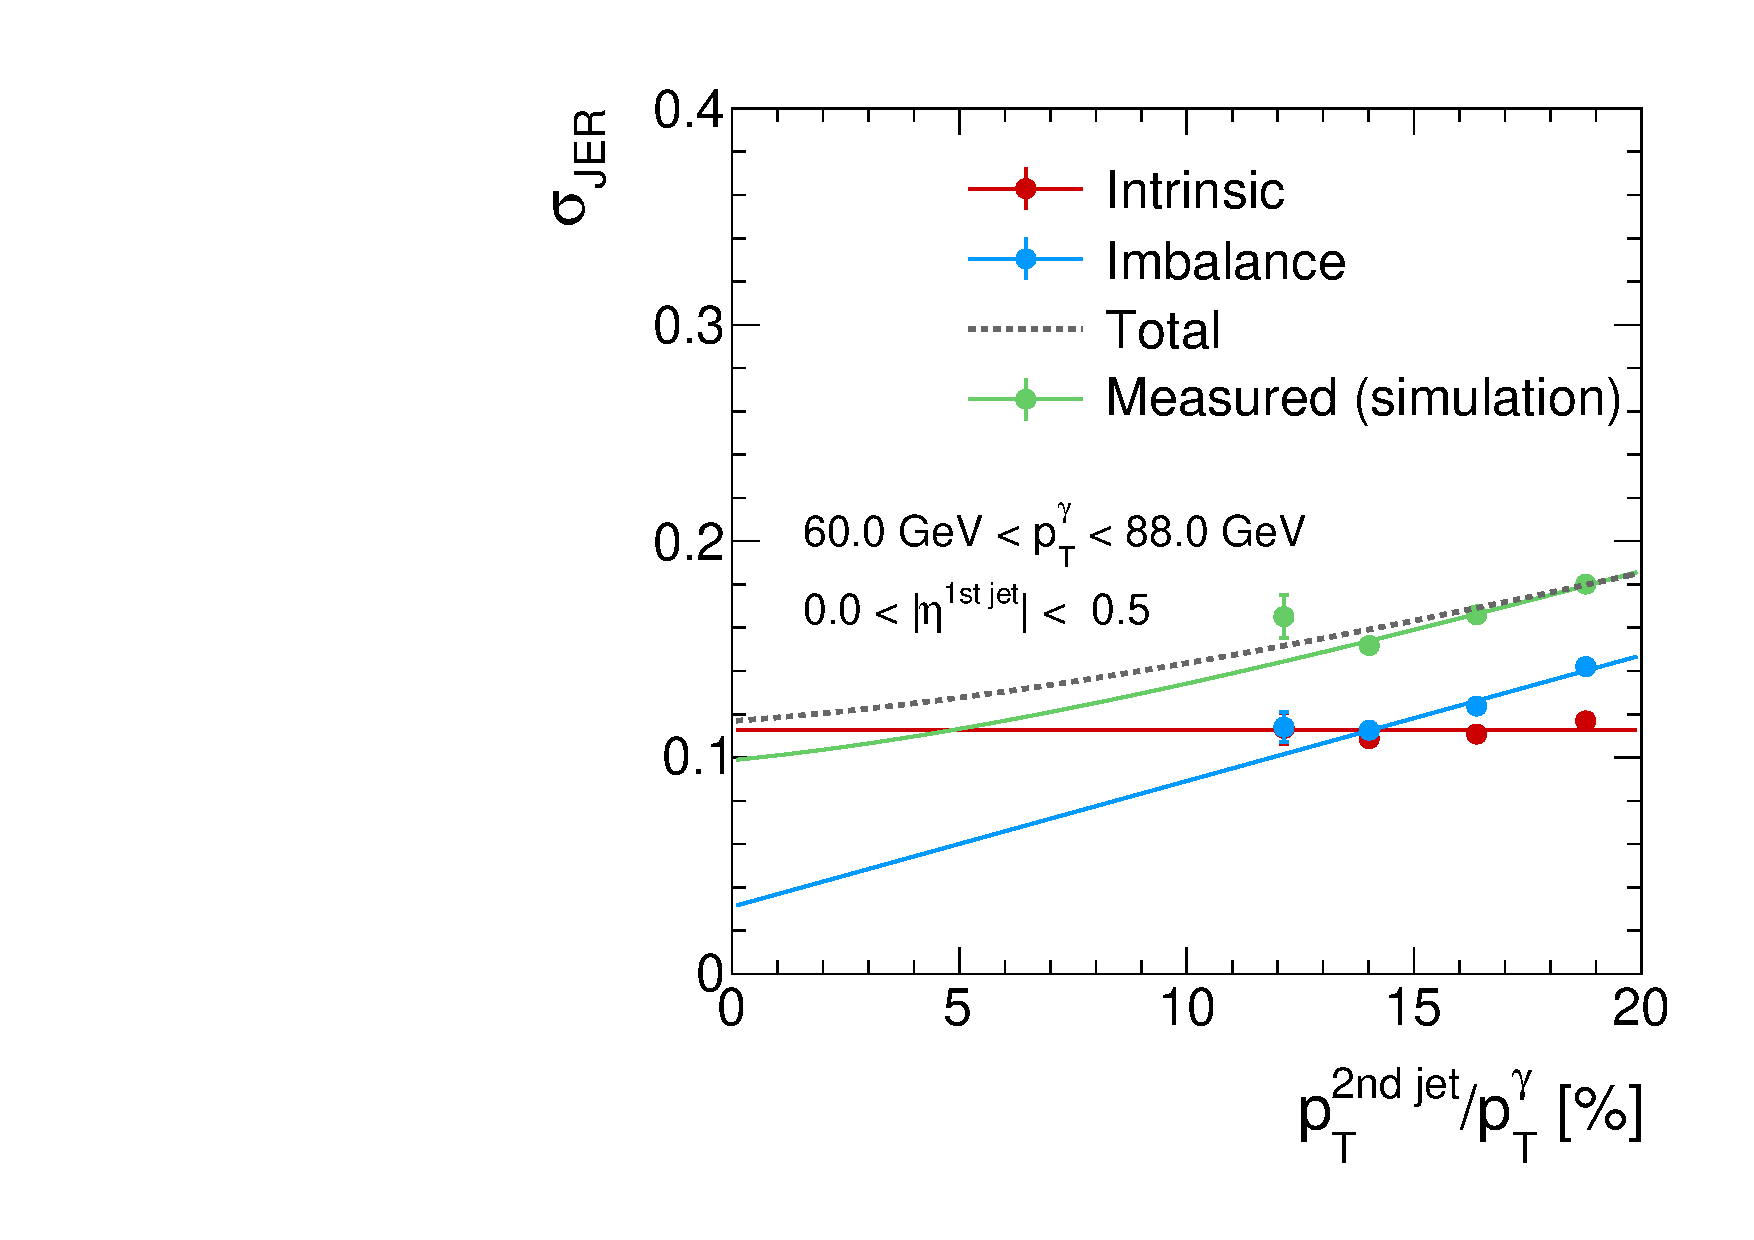
\includegraphics[width=0.32\textwidth]{figures/resolution/results/JER_for_1_eta_bin_3_pTGamma_bin_all_contributions_PFCHS_RMS99_mc.pdf}
    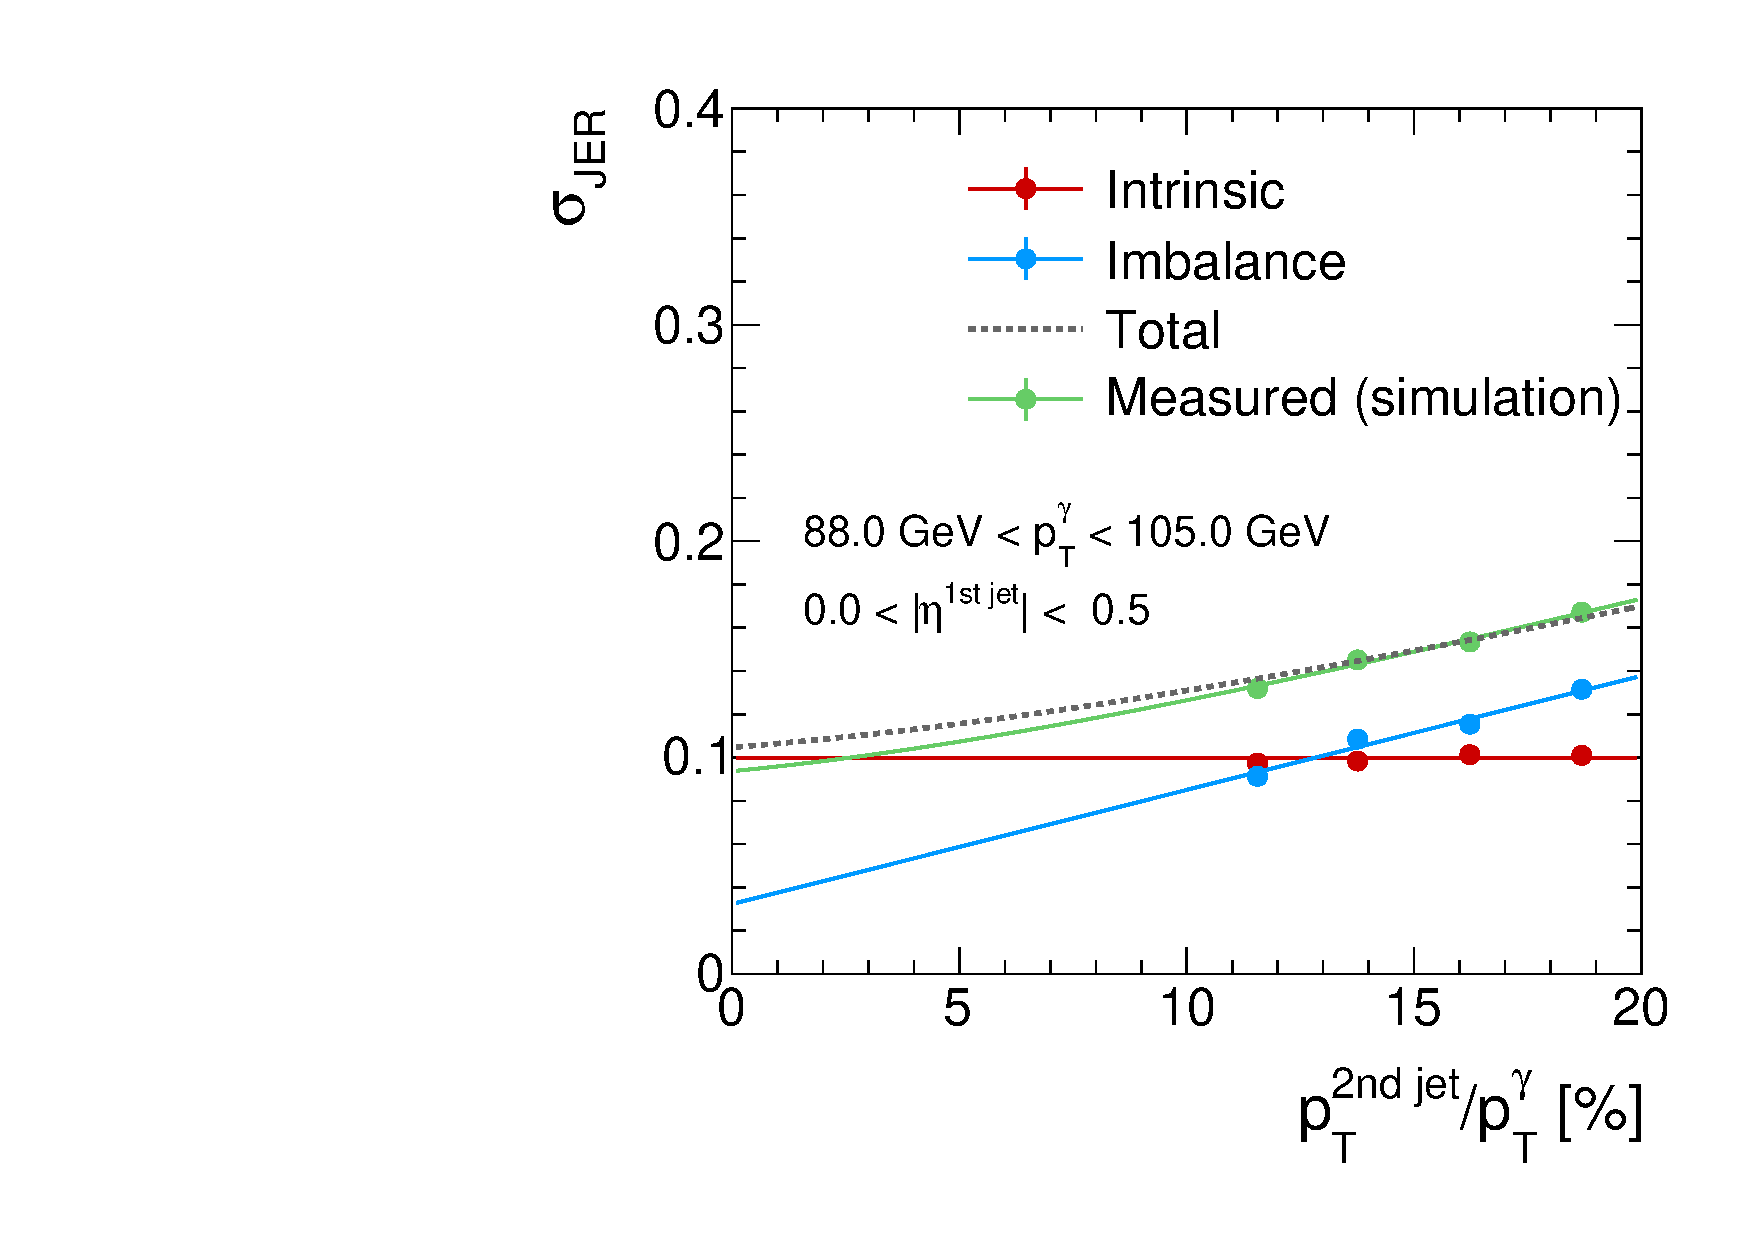
\includegraphics[width=0.32\textwidth]{figures/resolution/results/JER_for_1_eta_bin_4_pTGamma_bin_all_contributions_PFCHS_RMS99_mc.pdf}
    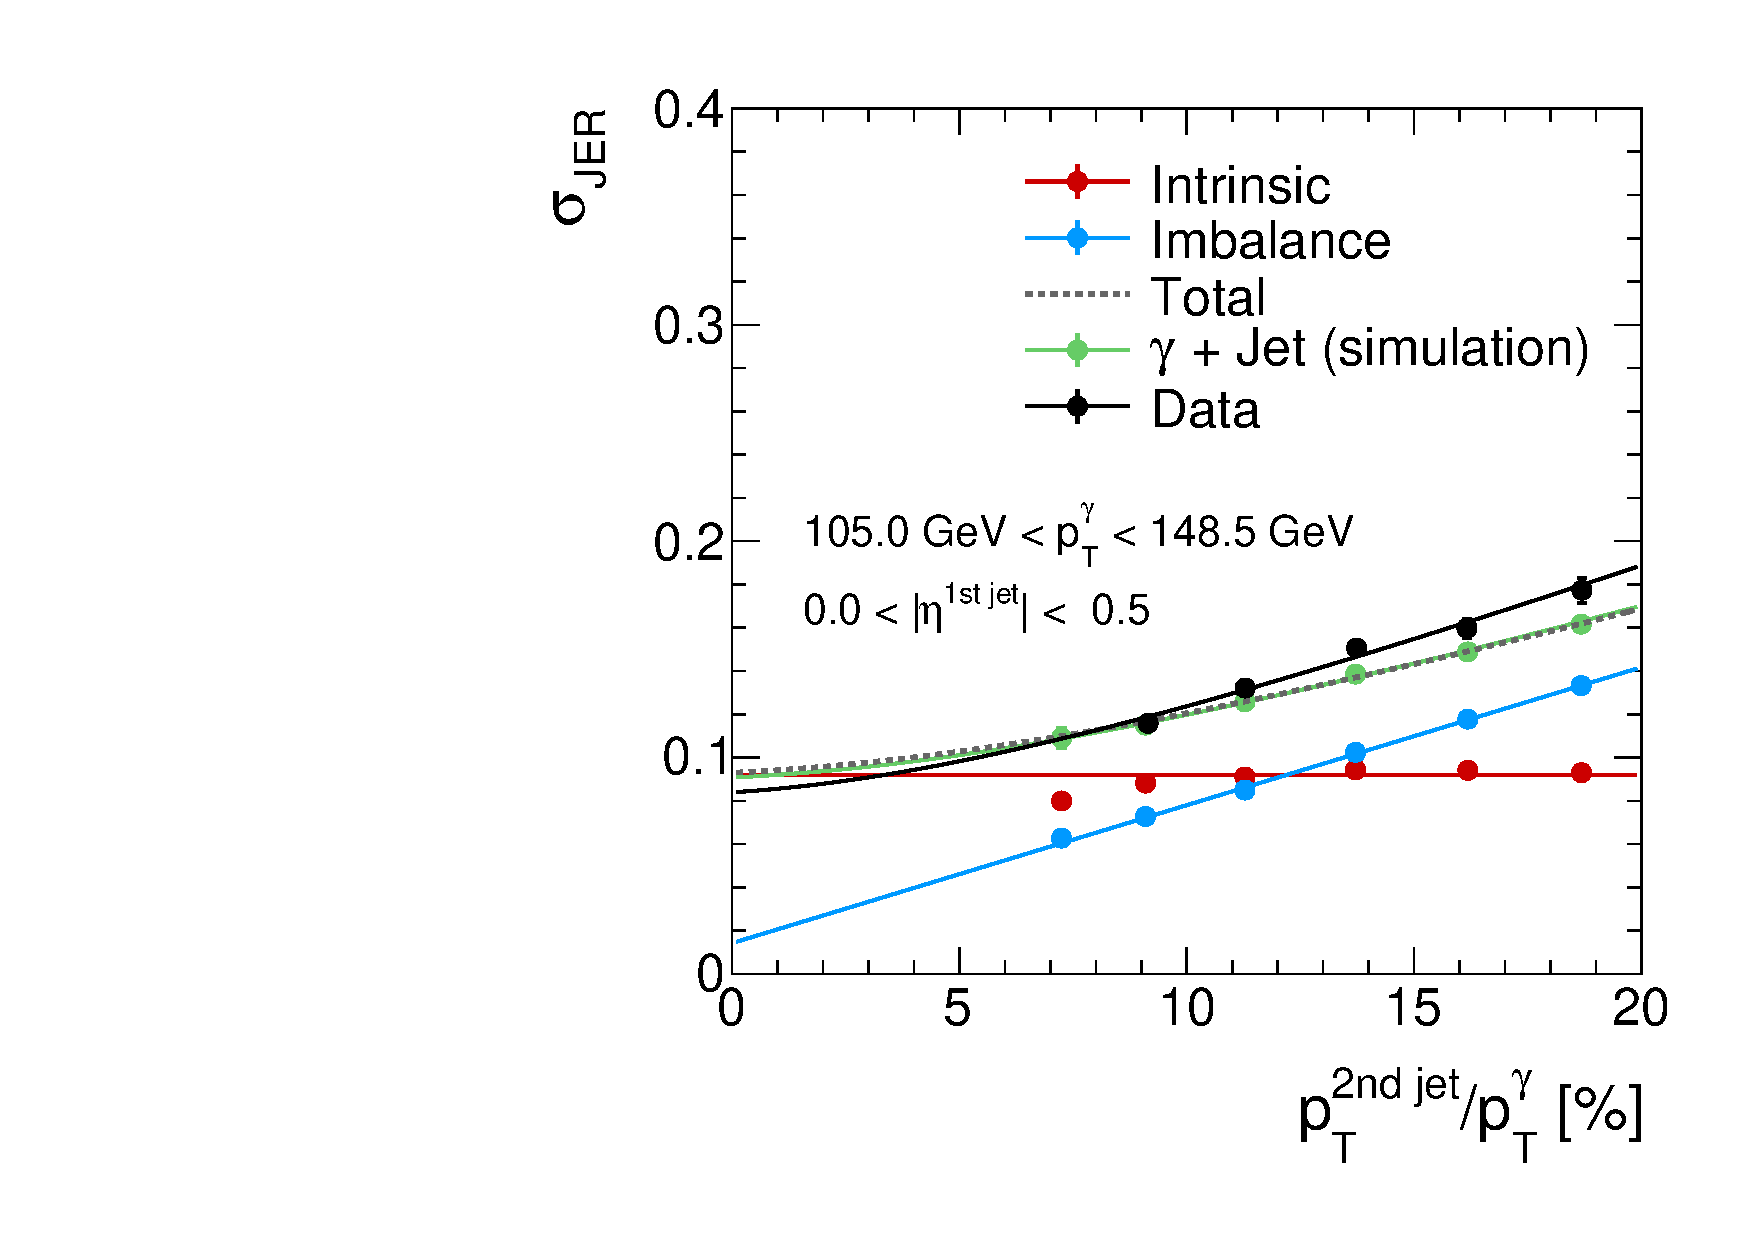
\includegraphics[width=0.32\textwidth]{figures/resolution/results/JER_for_1_eta_bin_5_pTGamma_bin_all_contributions_PFCHS_RMS99_mc.pdf}

    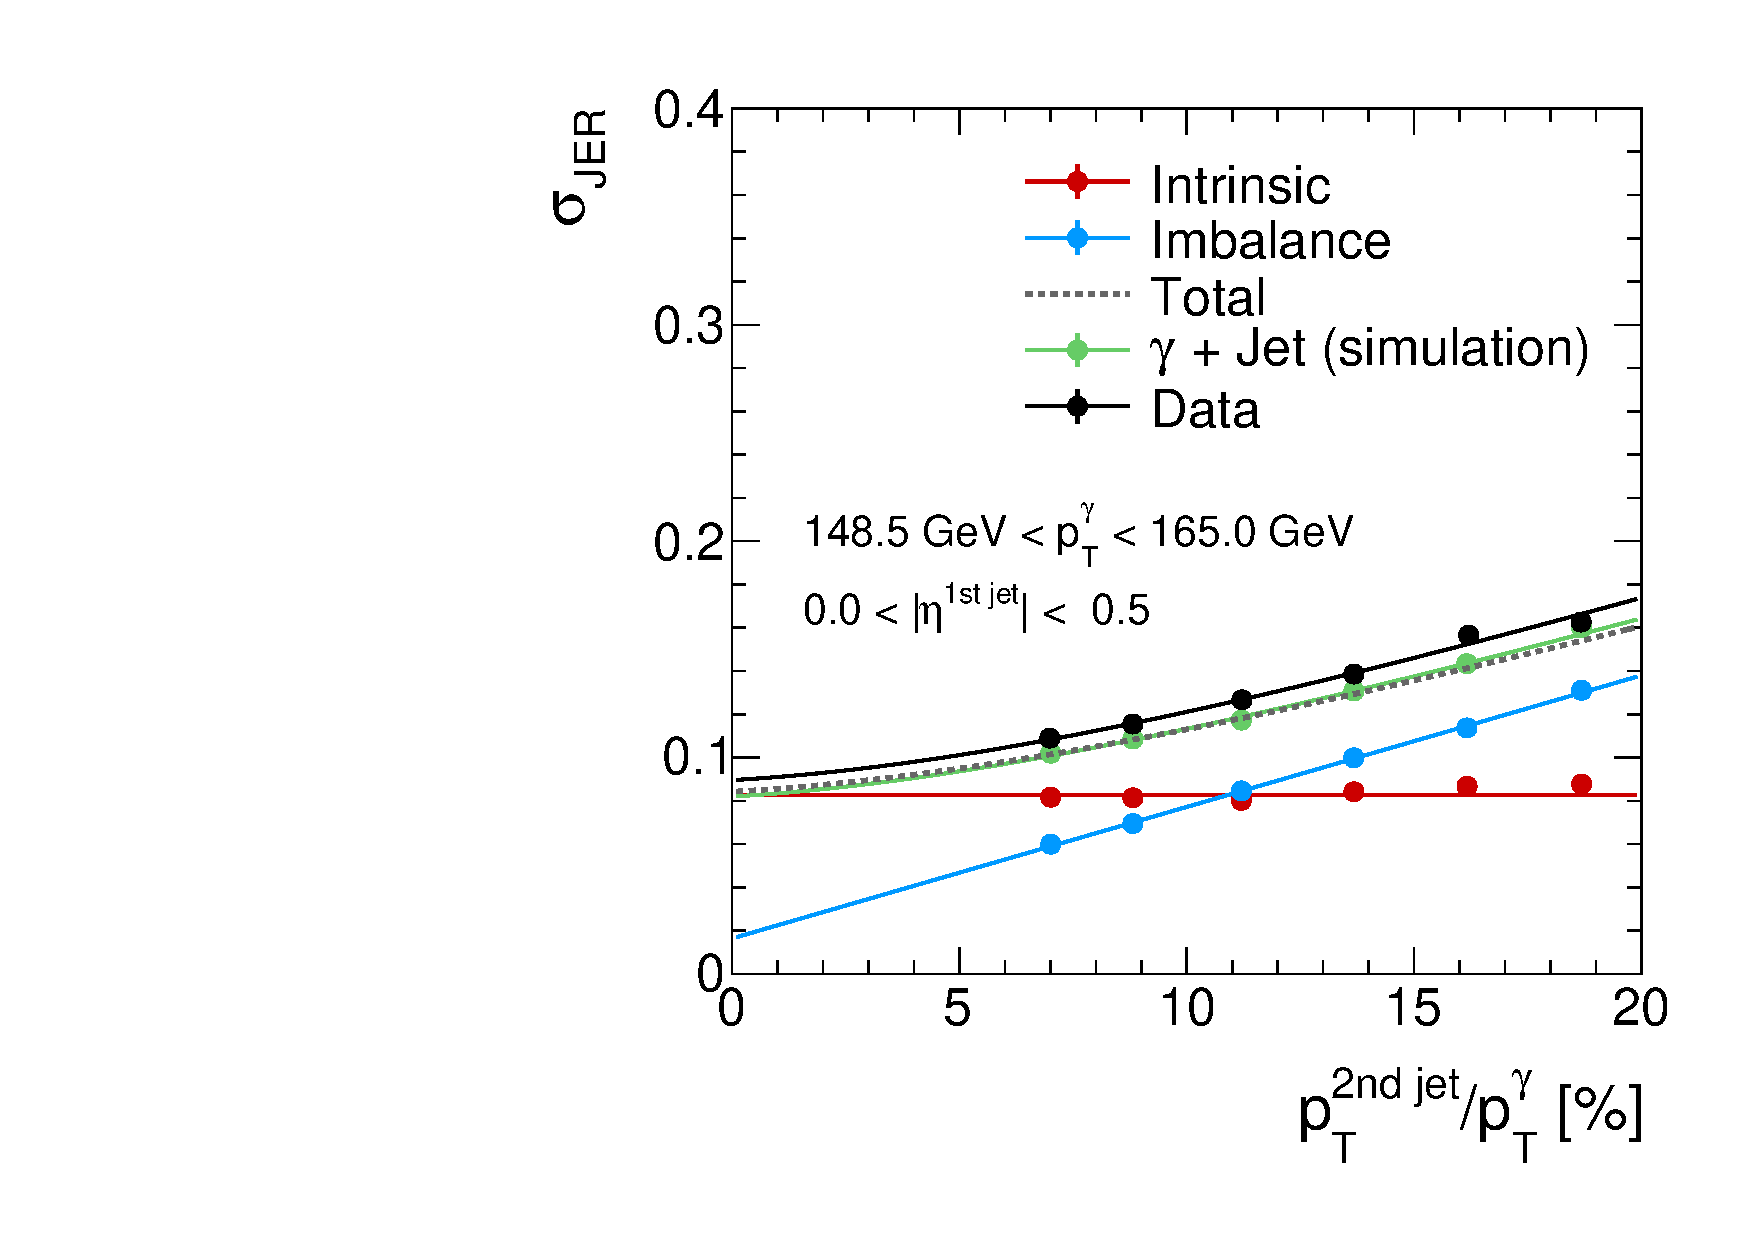
\includegraphics[width=0.32\textwidth]{figures/resolution/results/JER_for_1_eta_bin_6_pTGamma_bin_all_contributions_PFCHS_RMS99_mc.pdf}
    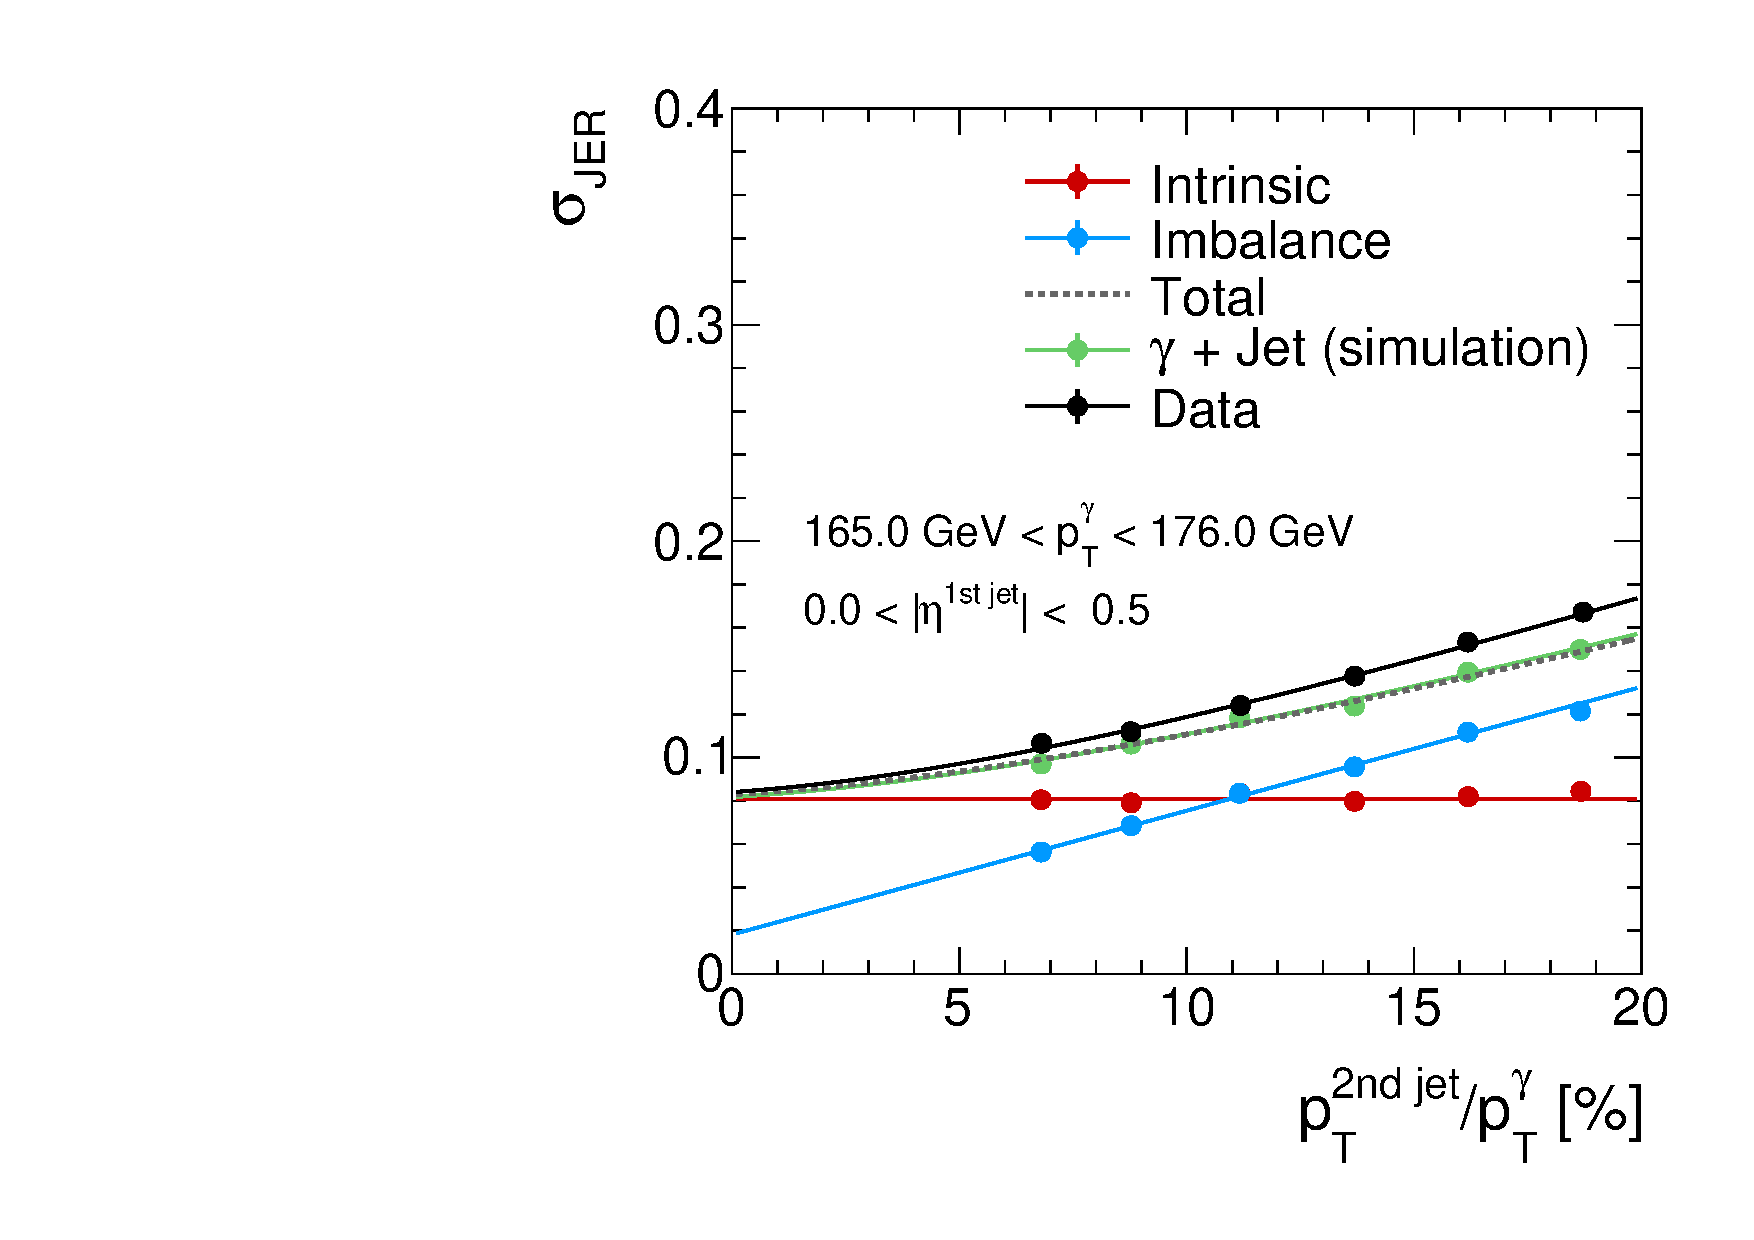
\includegraphics[width=0.32\textwidth]{figures/resolution/results/JER_for_1_eta_bin_7_pTGamma_bin_all_contributions_PFCHS_RMS99_mc.pdf}
    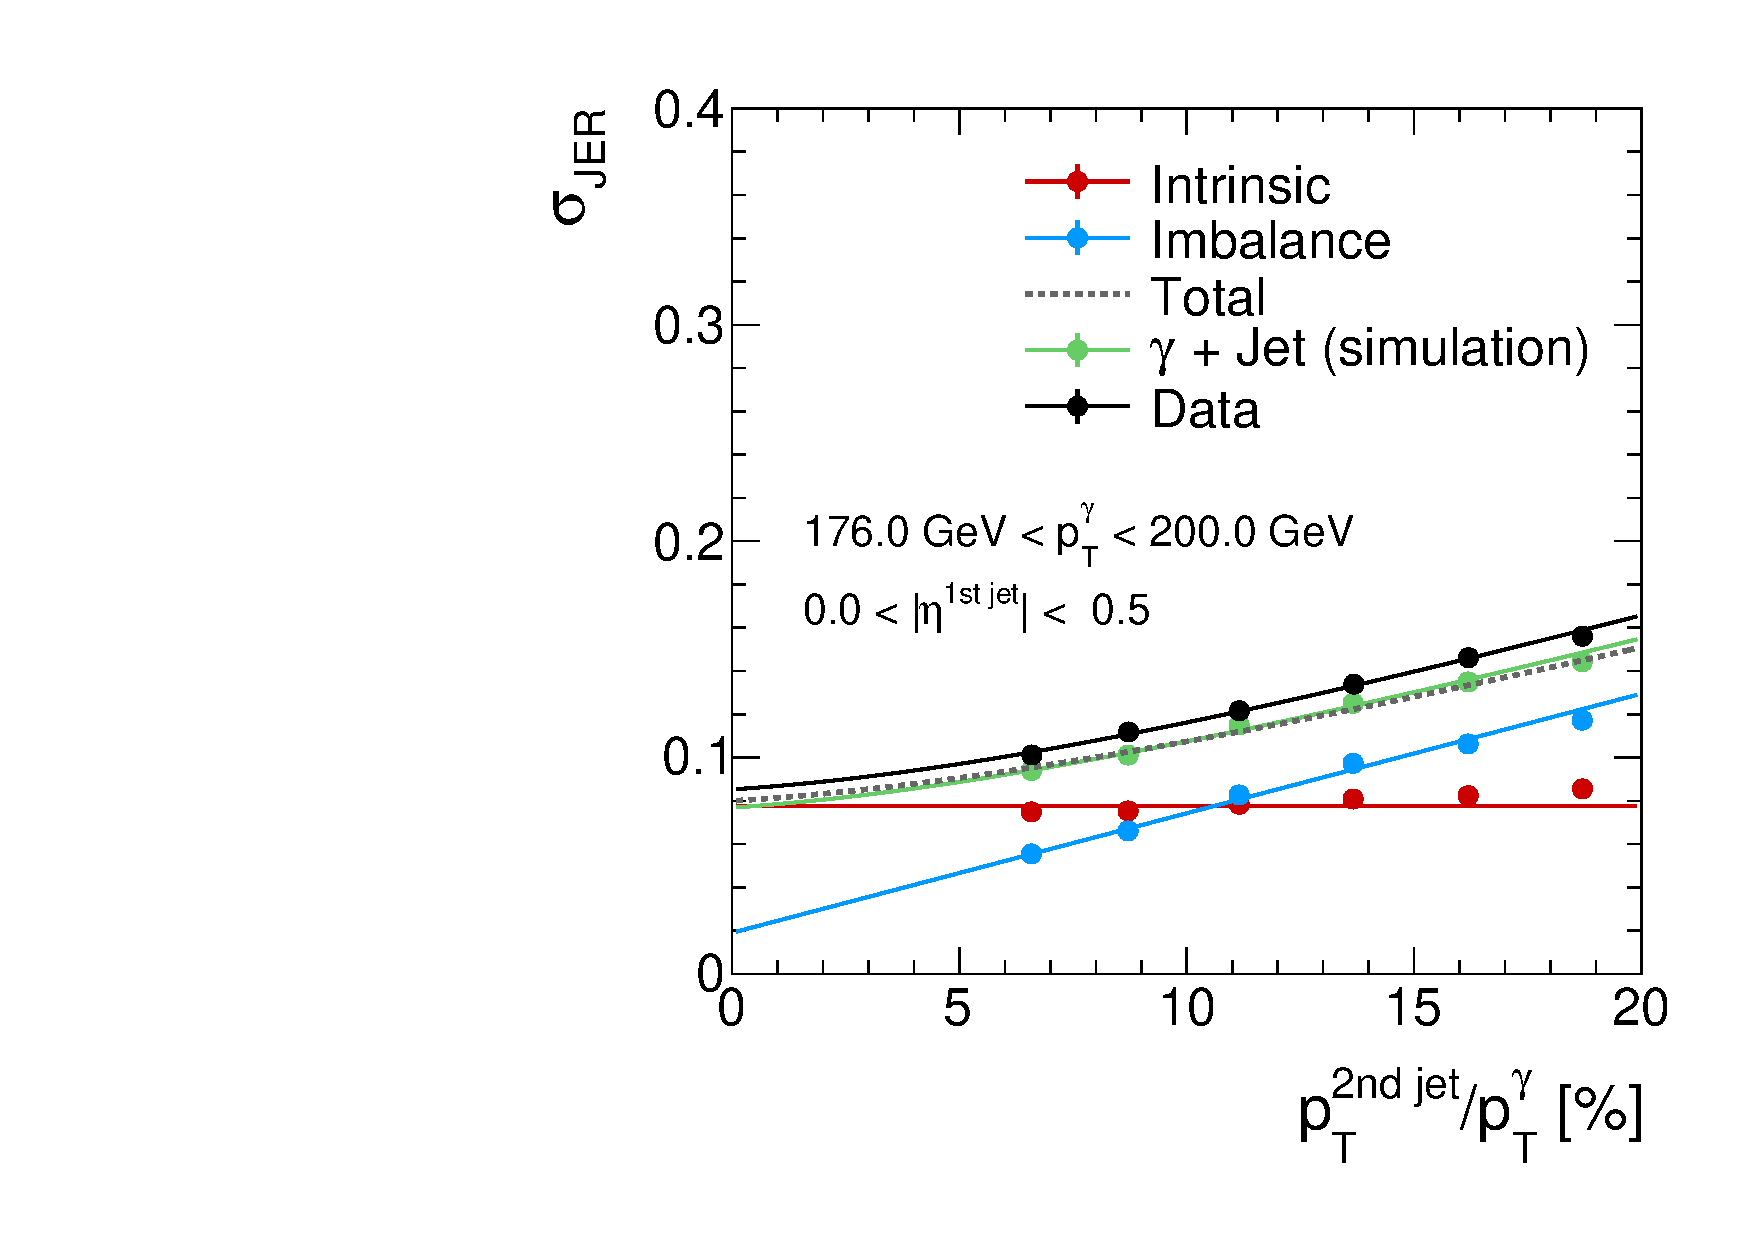
\includegraphics[width=0.32\textwidth]{figures/resolution/results/JER_for_1_eta_bin_8_pTGamma_bin_all_contributions_PFCHS_RMS99_mc.pdf}

    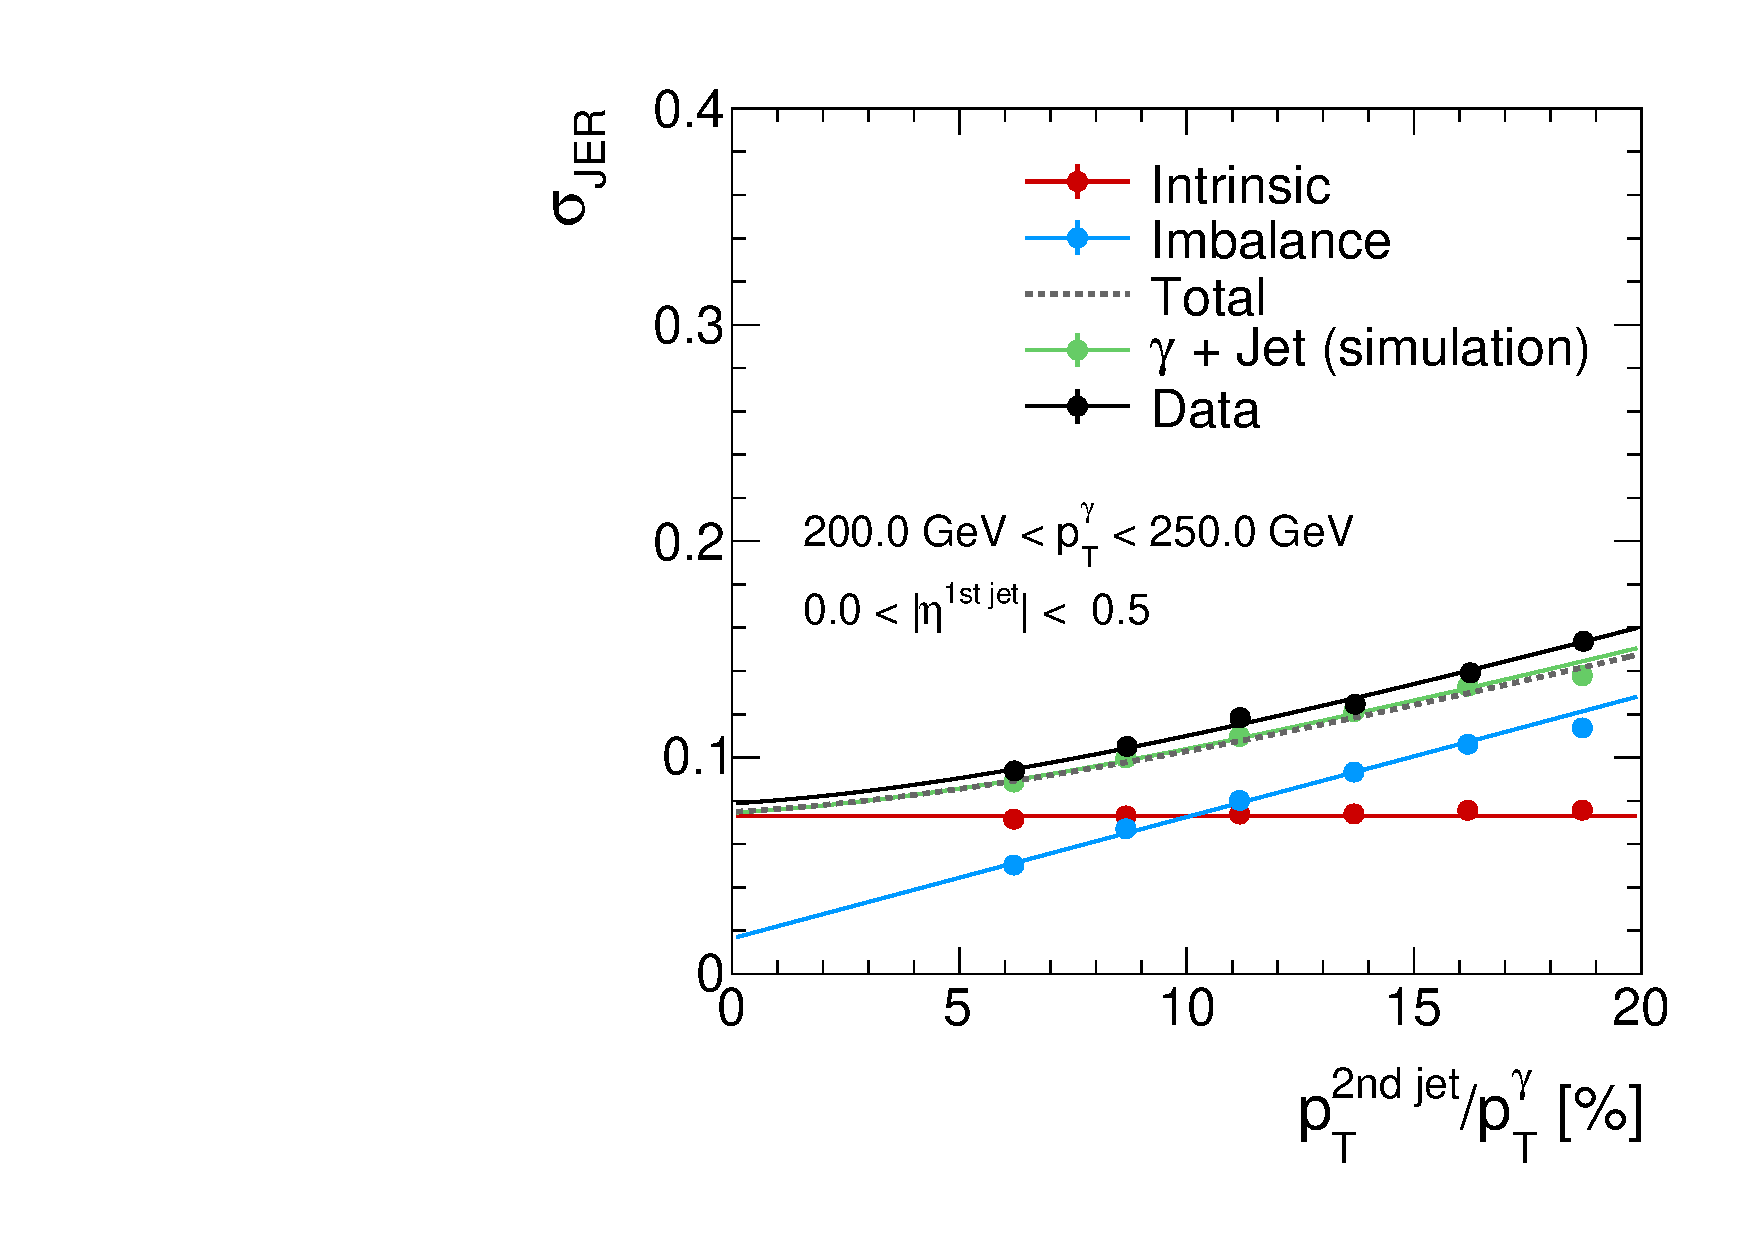
\includegraphics[width=0.32\textwidth]{figures/resolution/results/JER_for_1_eta_bin_9_pTGamma_bin_all_contributions_PFCHS_RMS99_mc.pdf}
    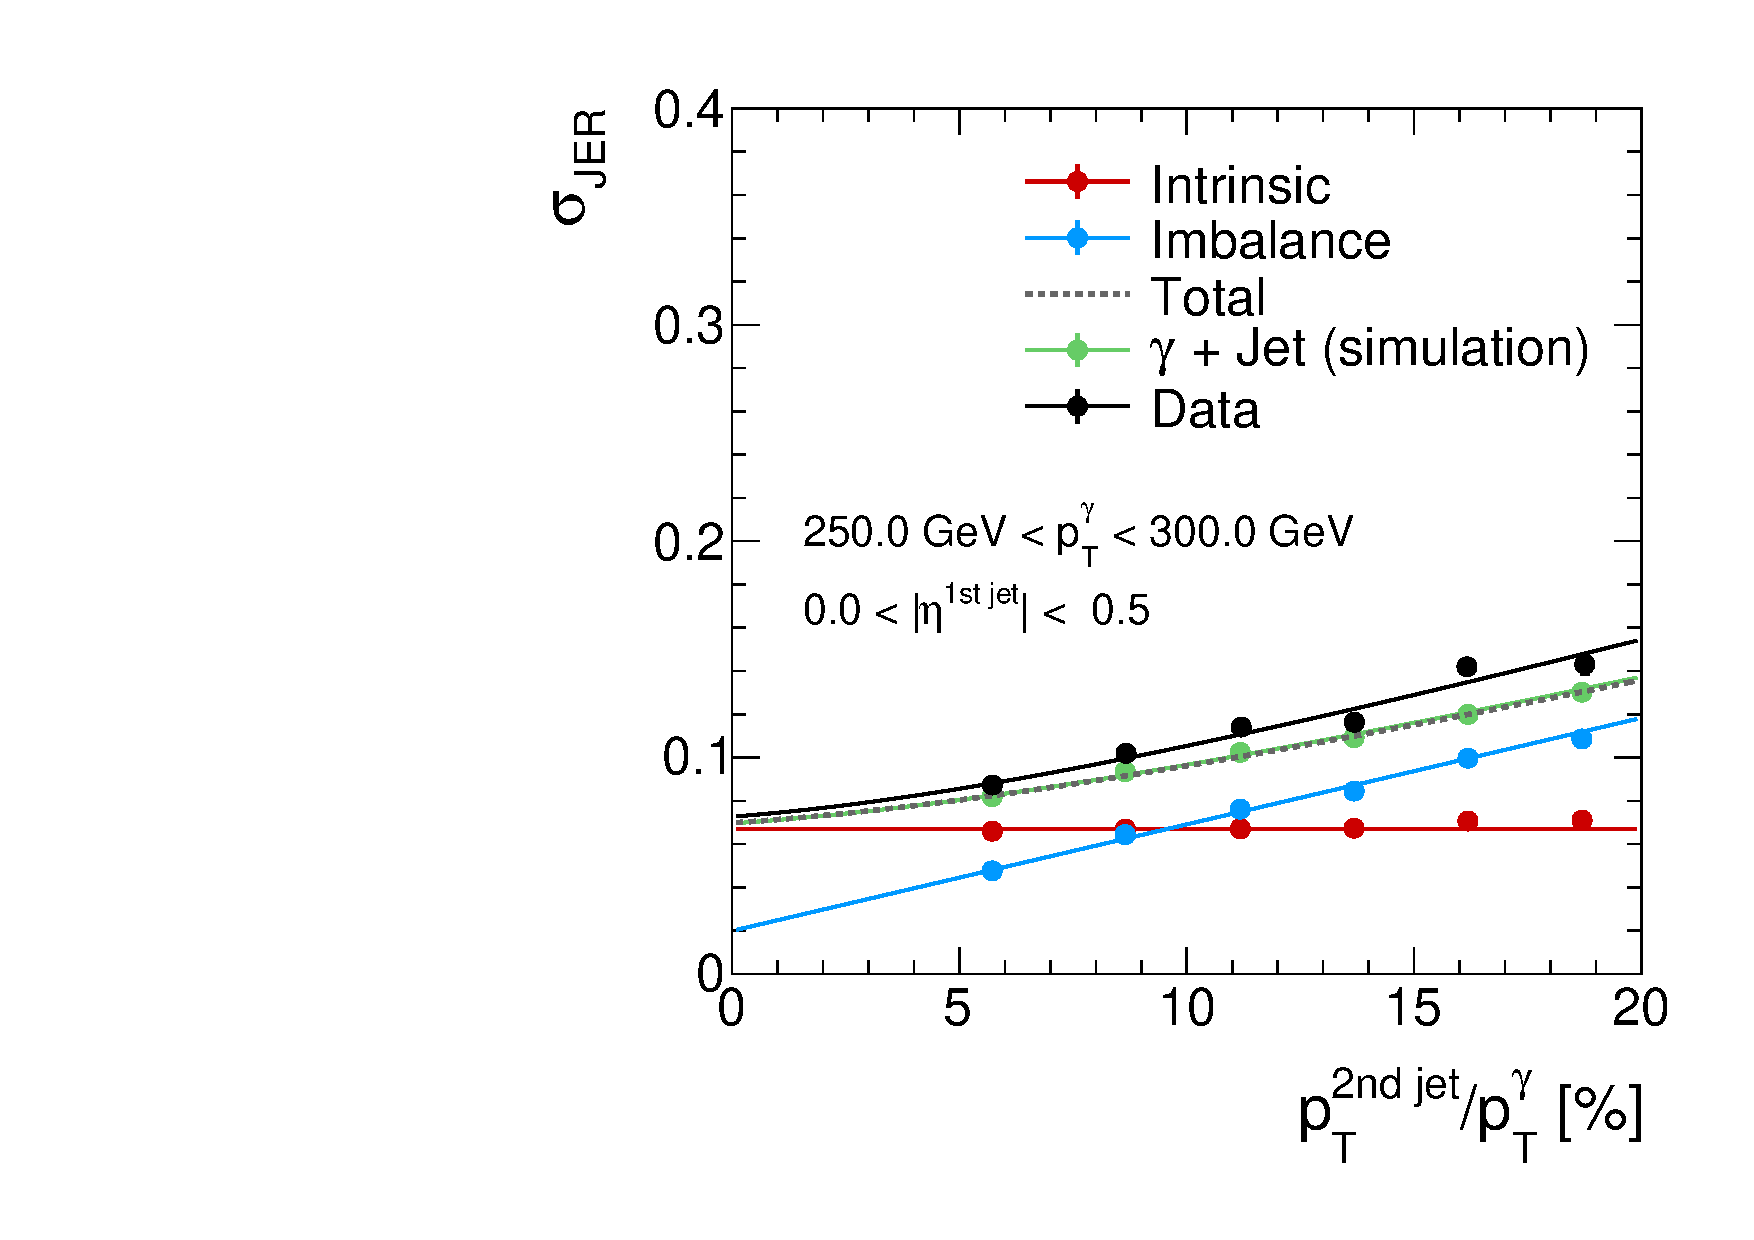
\includegraphics[width=0.32\textwidth]{figures/resolution/results/JER_for_1_eta_bin_10_pTGamma_bin_all_contributions_PFCHS_RMS99_mc.pdf}
    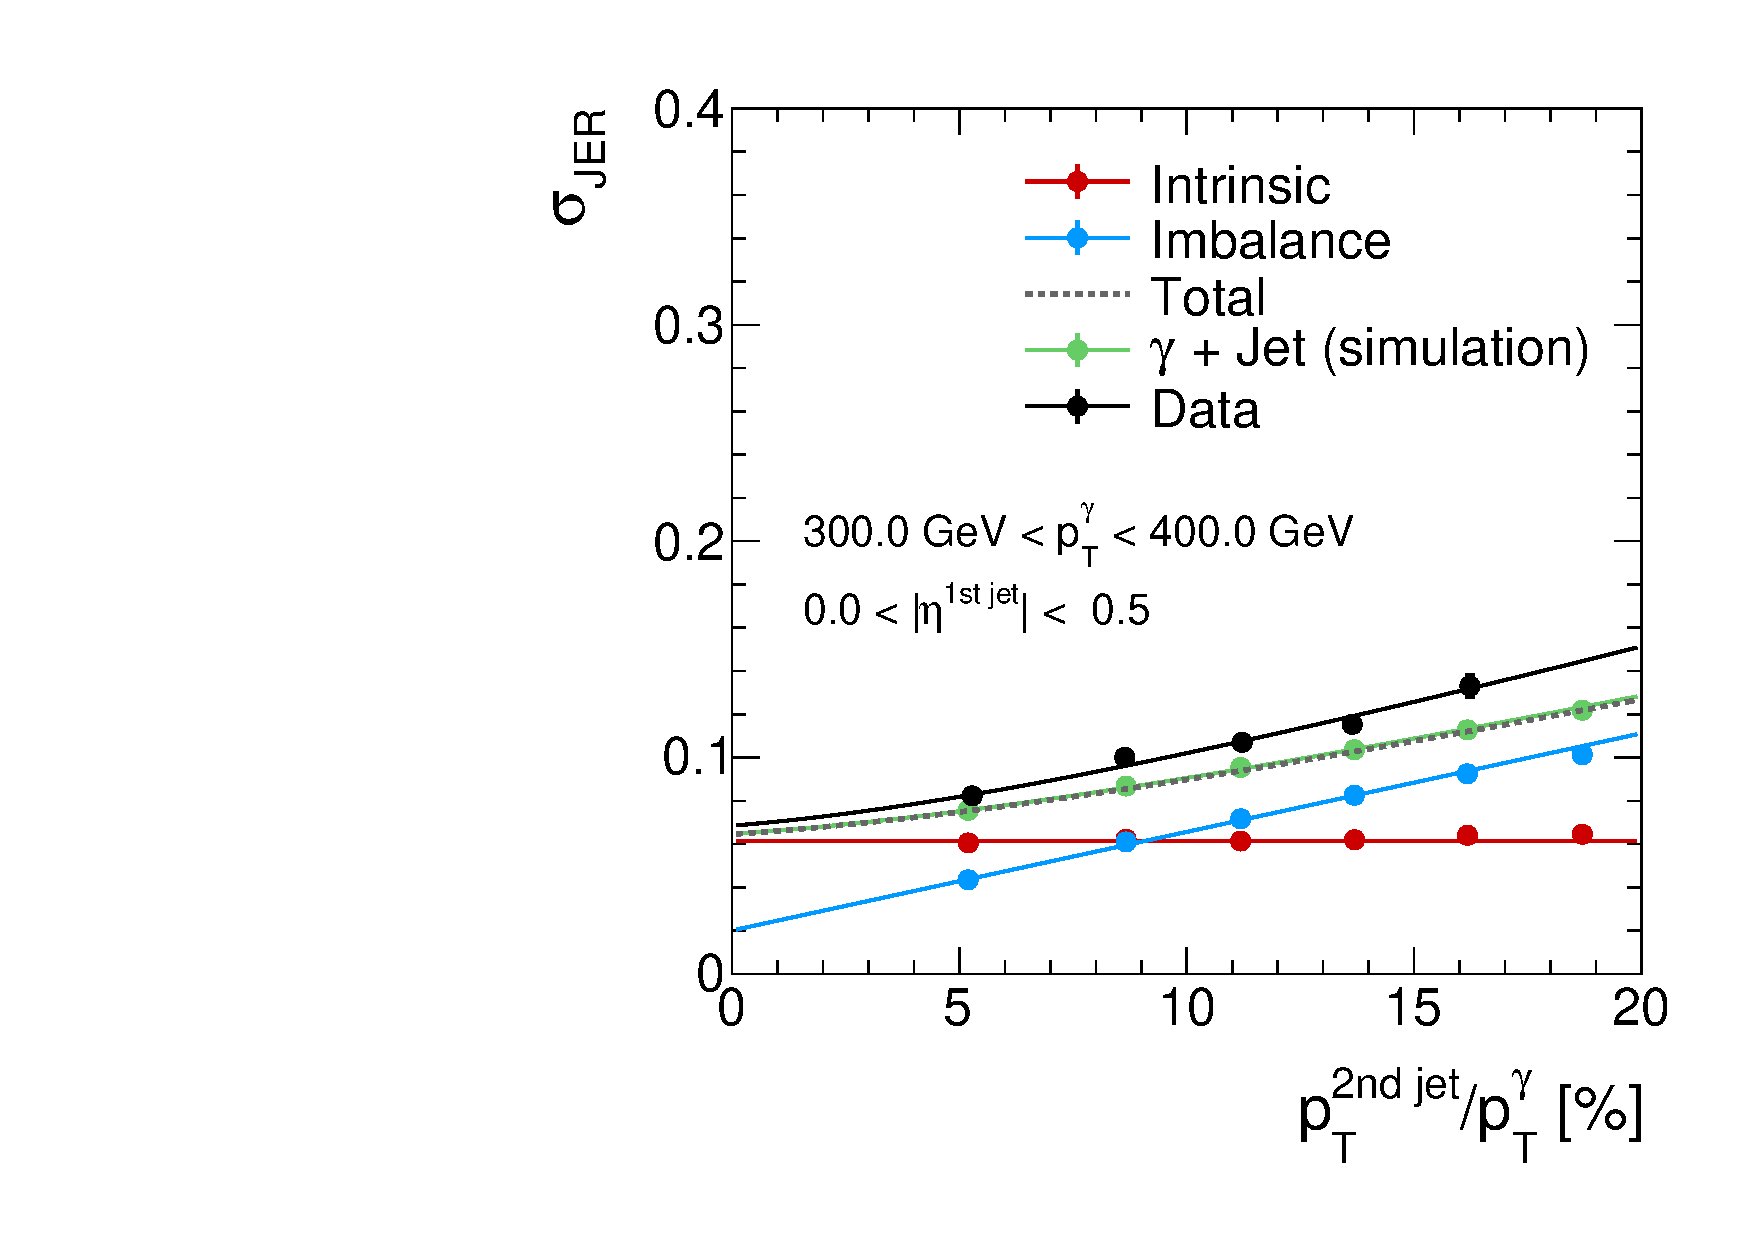
\includegraphics[width=0.32\textwidth]{figures/resolution/results/JER_for_1_eta_bin_11_pTGamma_bin_all_contributions_PFCHS_RMS99_mc.pdf}
  \caption{\jer($\alpha$) of the intrinsic, imbalance and total resolution in simulation and the resolution measured in data for all $|\etafirstjet|$ and \ptgamma bins.}
  \label{fig:ExtrapolationPlots1}
\end{figure*}

\begin{figure*}[ht]
 \centering
    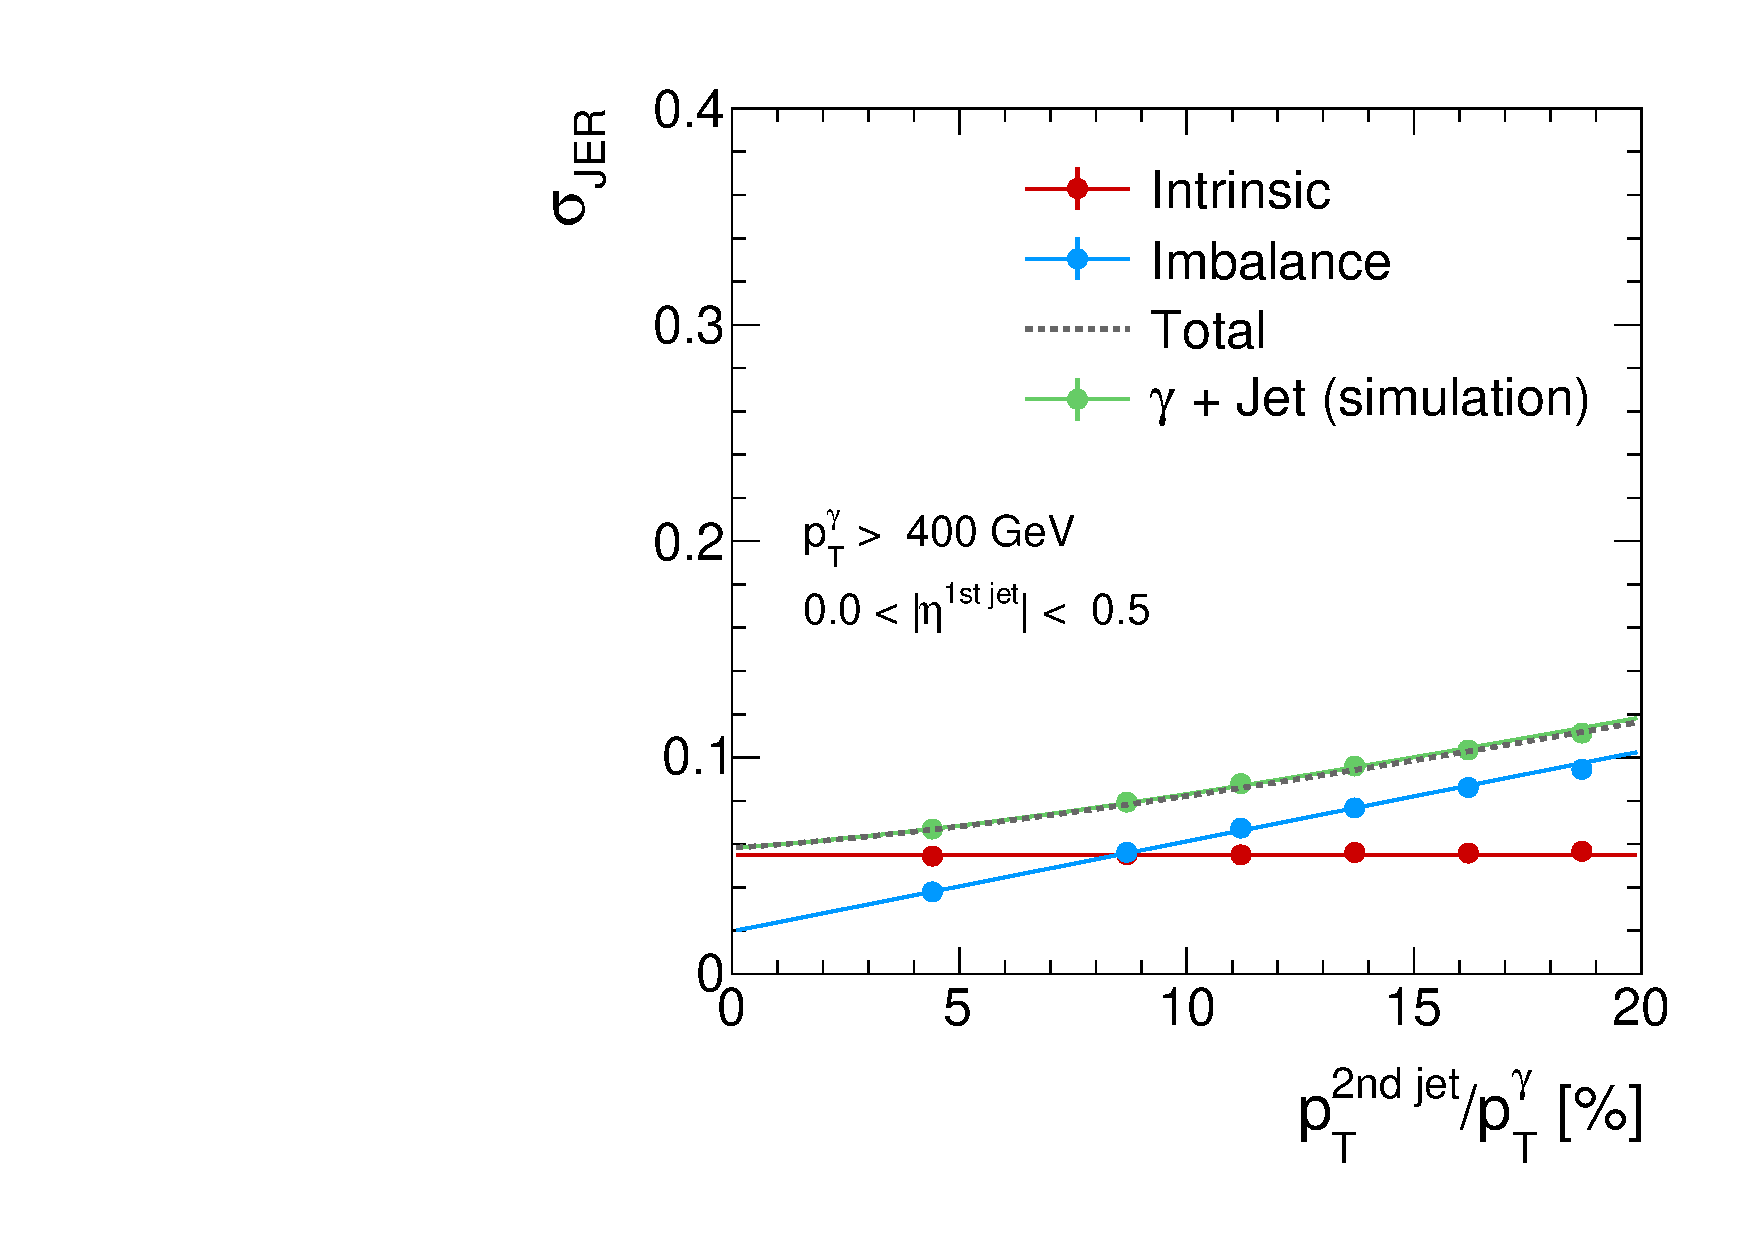
\includegraphics[width=0.32\textwidth]{figures/resolution/results/JER_for_1_eta_bin_12_pTGamma_bin_all_contributions_PFCHS_RMS99_mc.pdf}
    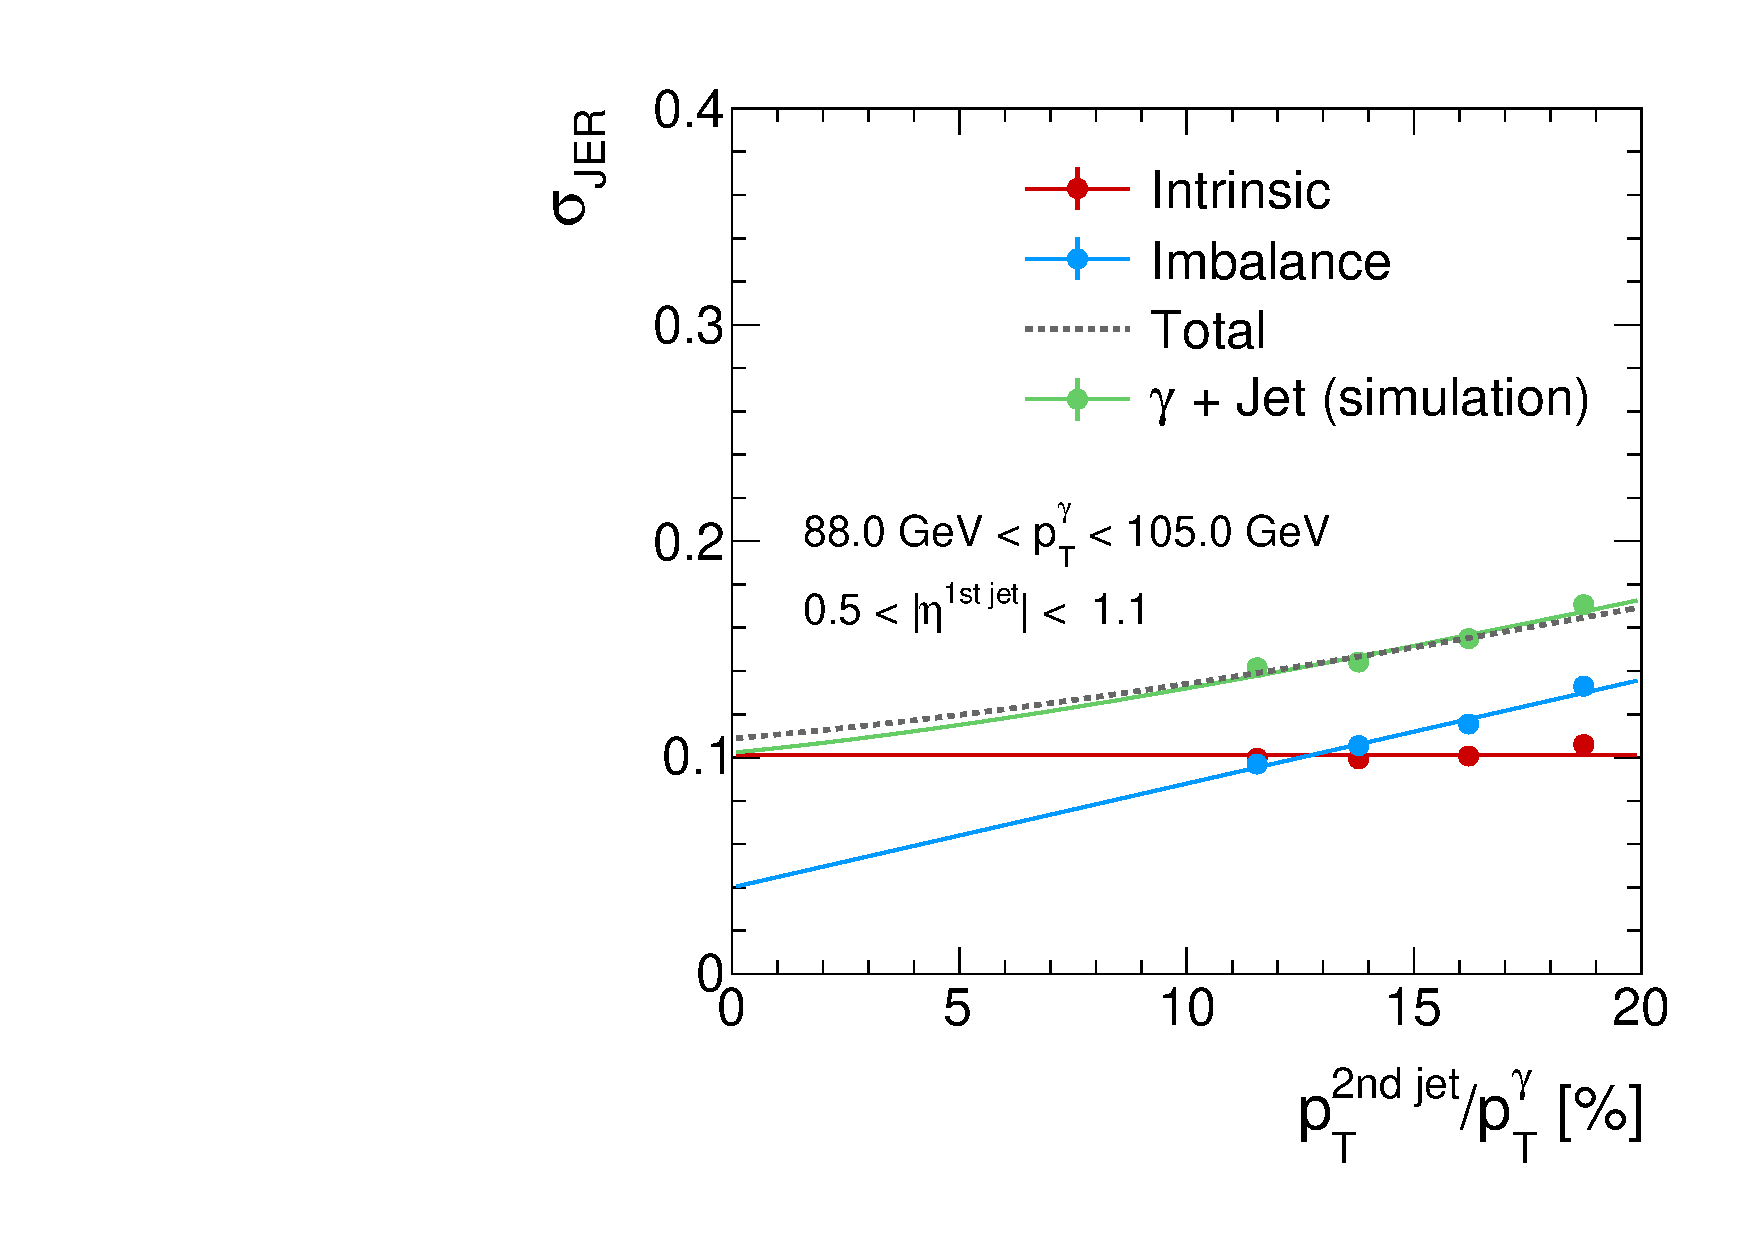
\includegraphics[width=0.32\textwidth]{figures/resolution/results/JER_for_2_eta_bin_4_pTGamma_bin_all_contributions_PFCHS_RMS99_mc.pdf}
    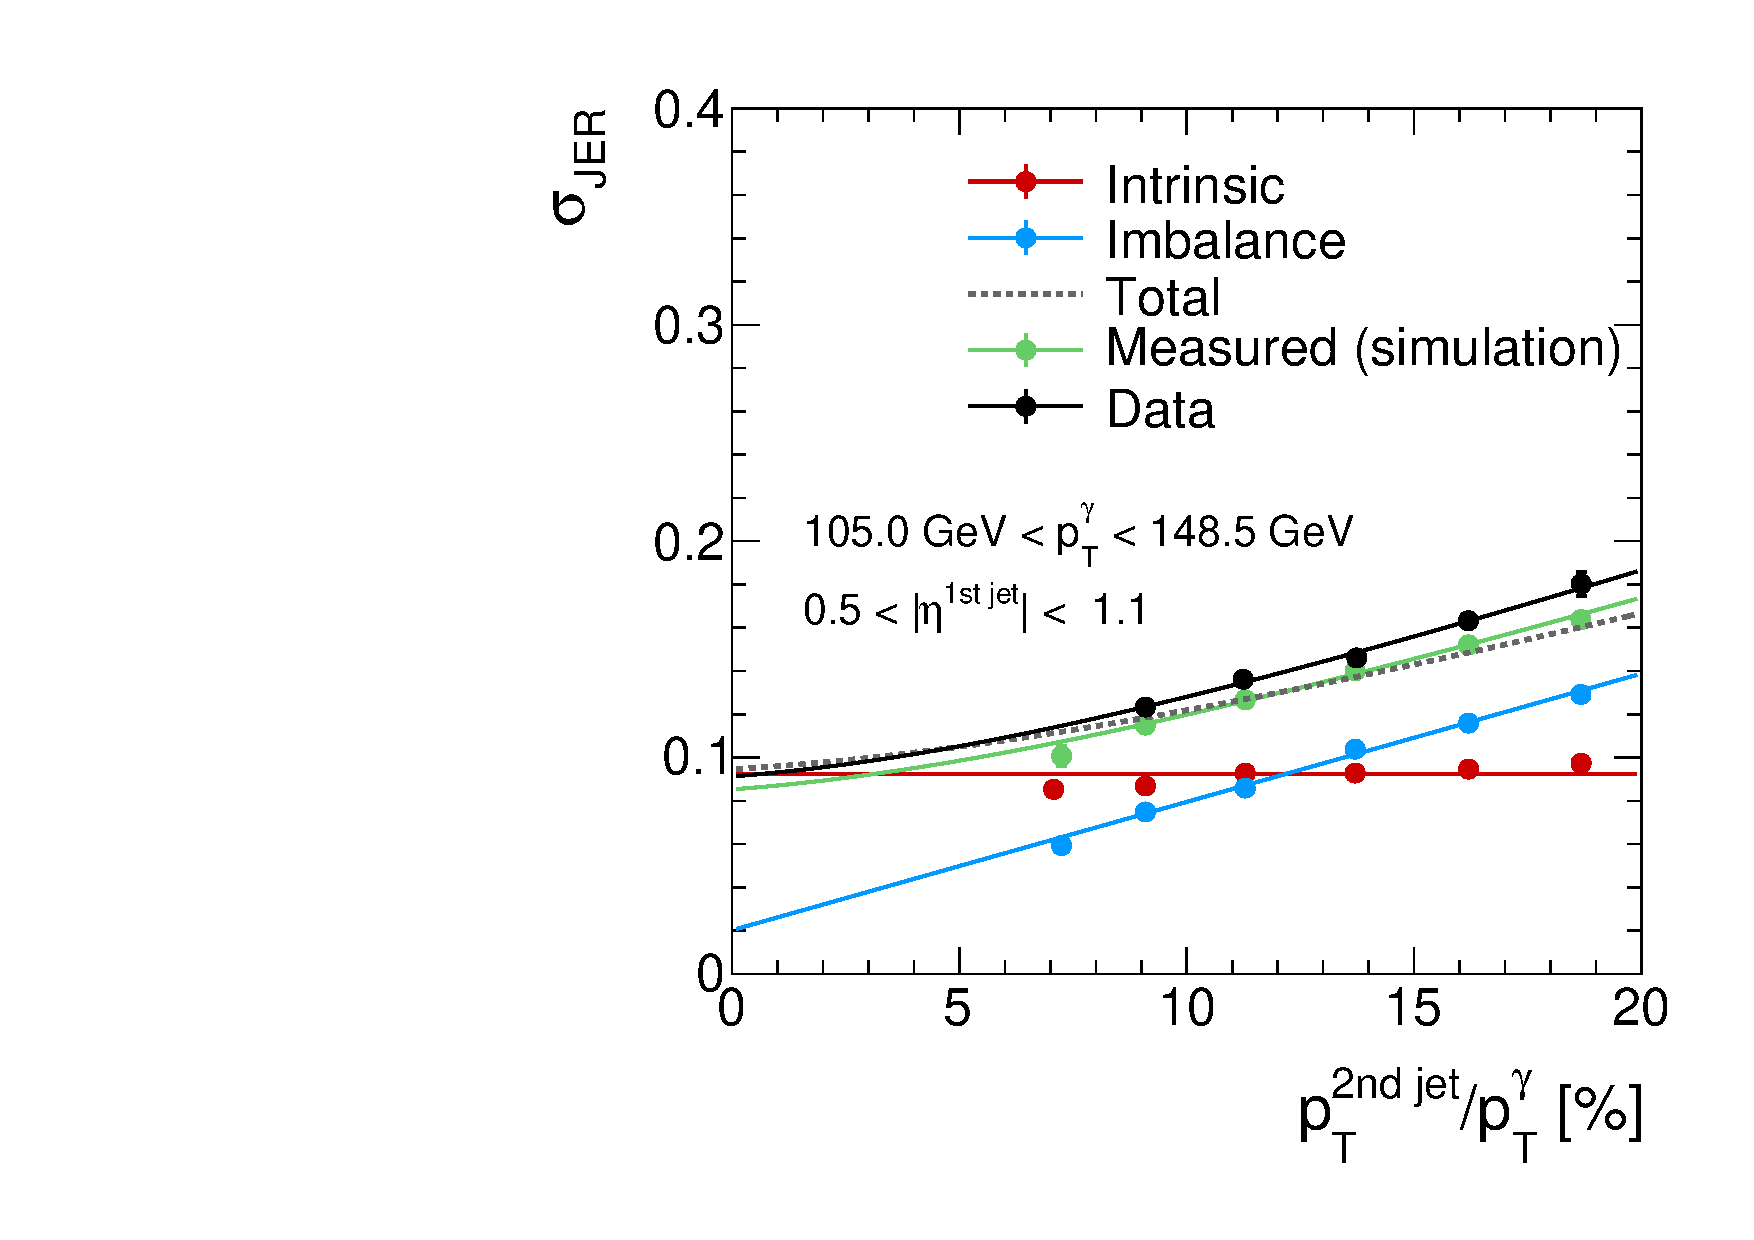
\includegraphics[width=0.32\textwidth]{figures/resolution/results/JER_for_2_eta_bin_5_pTGamma_bin_all_contributions_PFCHS_RMS99_mc.pdf}

    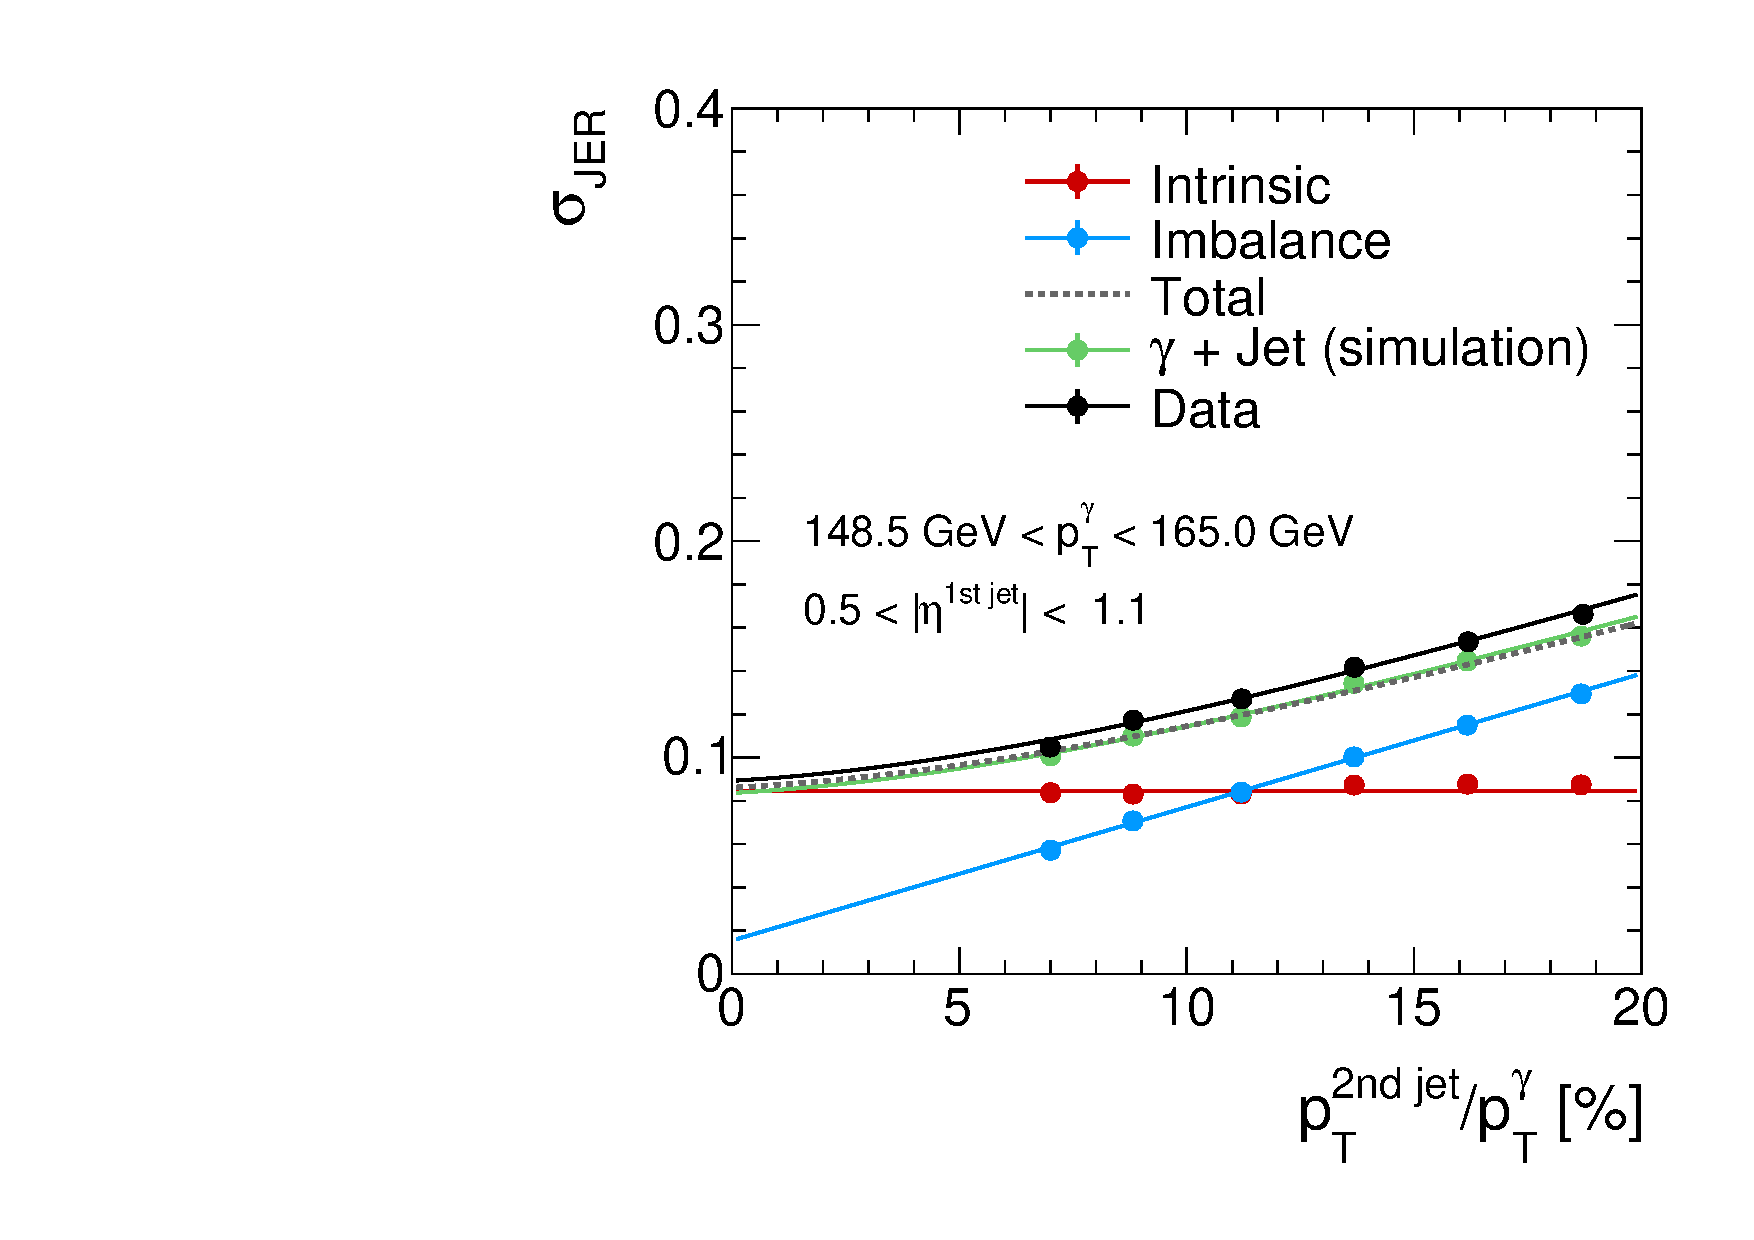
\includegraphics[width=0.32\textwidth]{figures/resolution/results/JER_for_2_eta_bin_6_pTGamma_bin_all_contributions_PFCHS_RMS99_mc.pdf}
    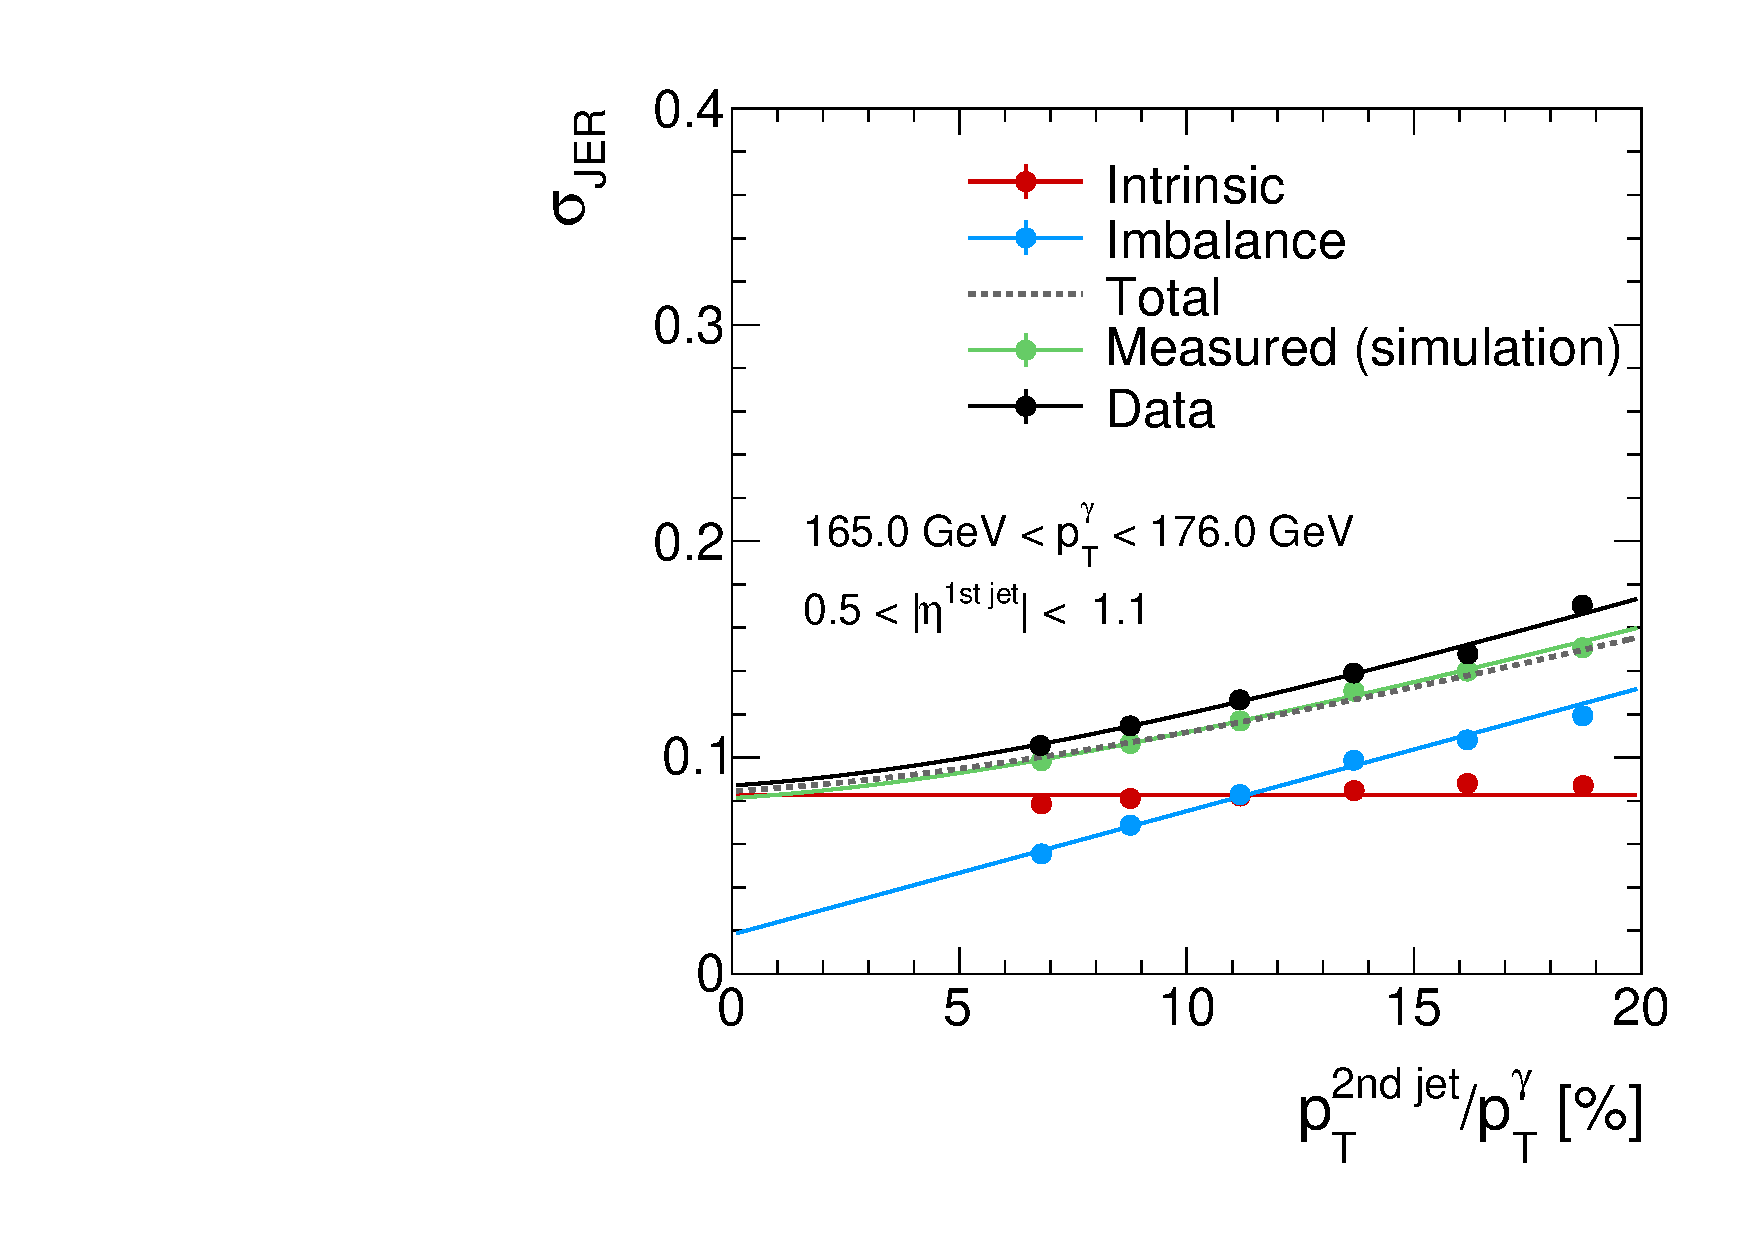
\includegraphics[width=0.32\textwidth]{figures/resolution/results/JER_for_2_eta_bin_7_pTGamma_bin_all_contributions_PFCHS_RMS99_mc.pdf}
    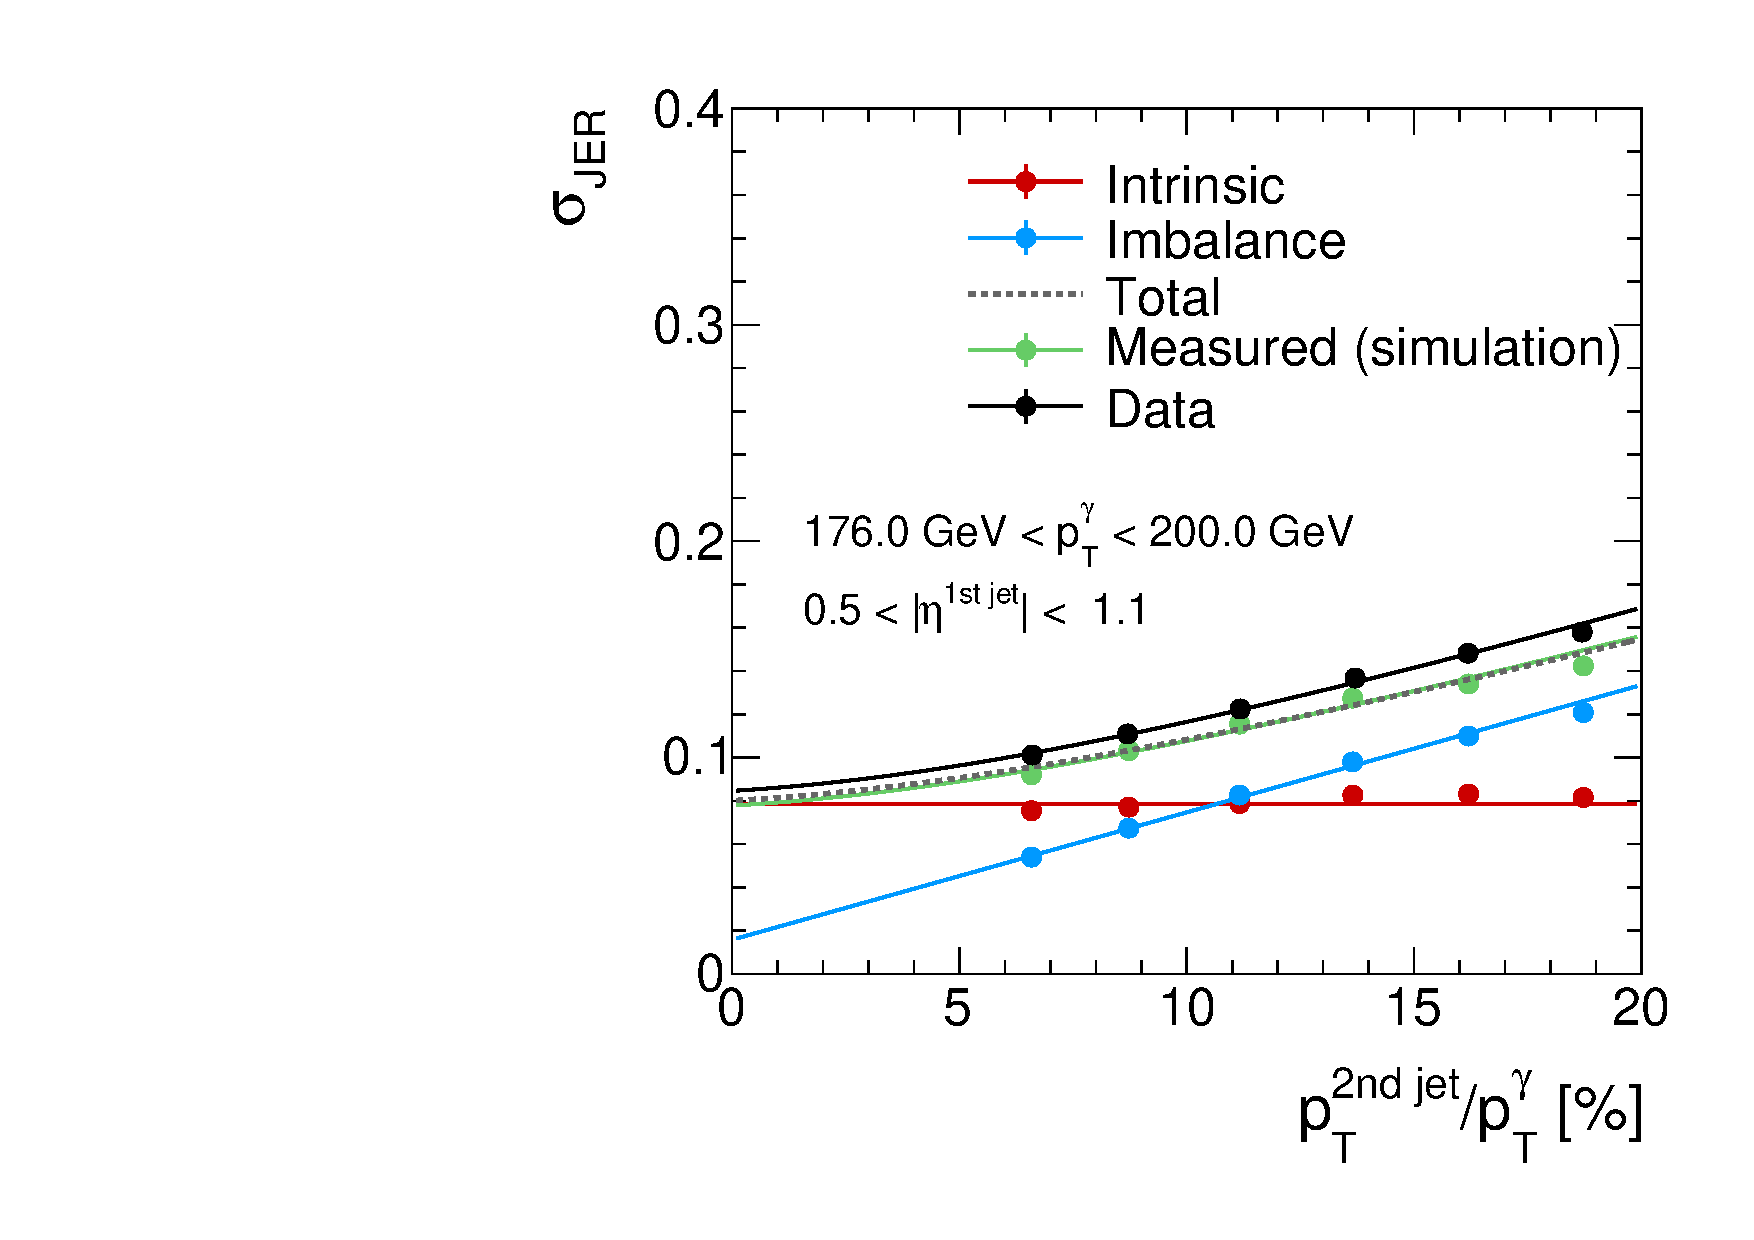
\includegraphics[width=0.32\textwidth]{figures/resolution/results/JER_for_2_eta_bin_8_pTGamma_bin_all_contributions_PFCHS_RMS99_mc.pdf}

    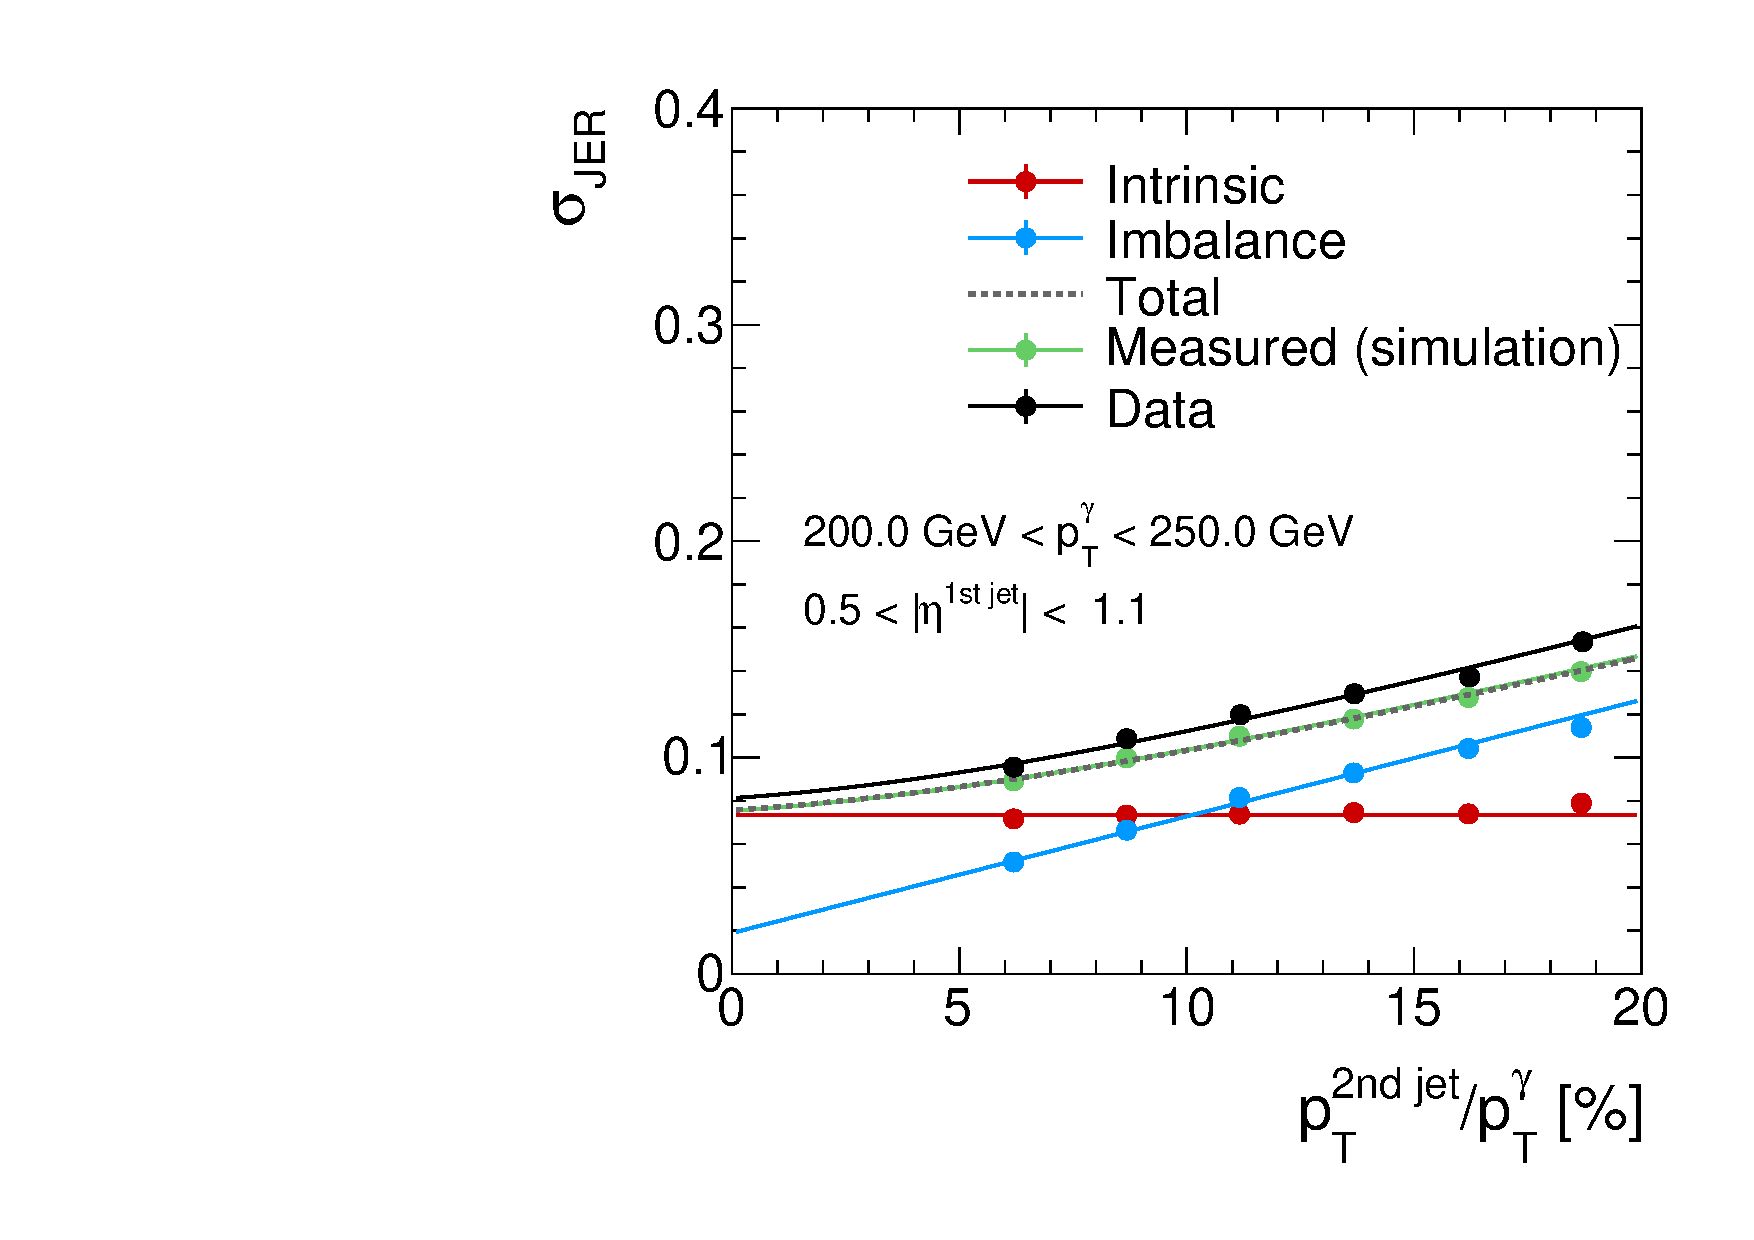
\includegraphics[width=0.32\textwidth]{figures/resolution/results/JER_for_2_eta_bin_9_pTGamma_bin_all_contributions_PFCHS_RMS99_mc.pdf}
    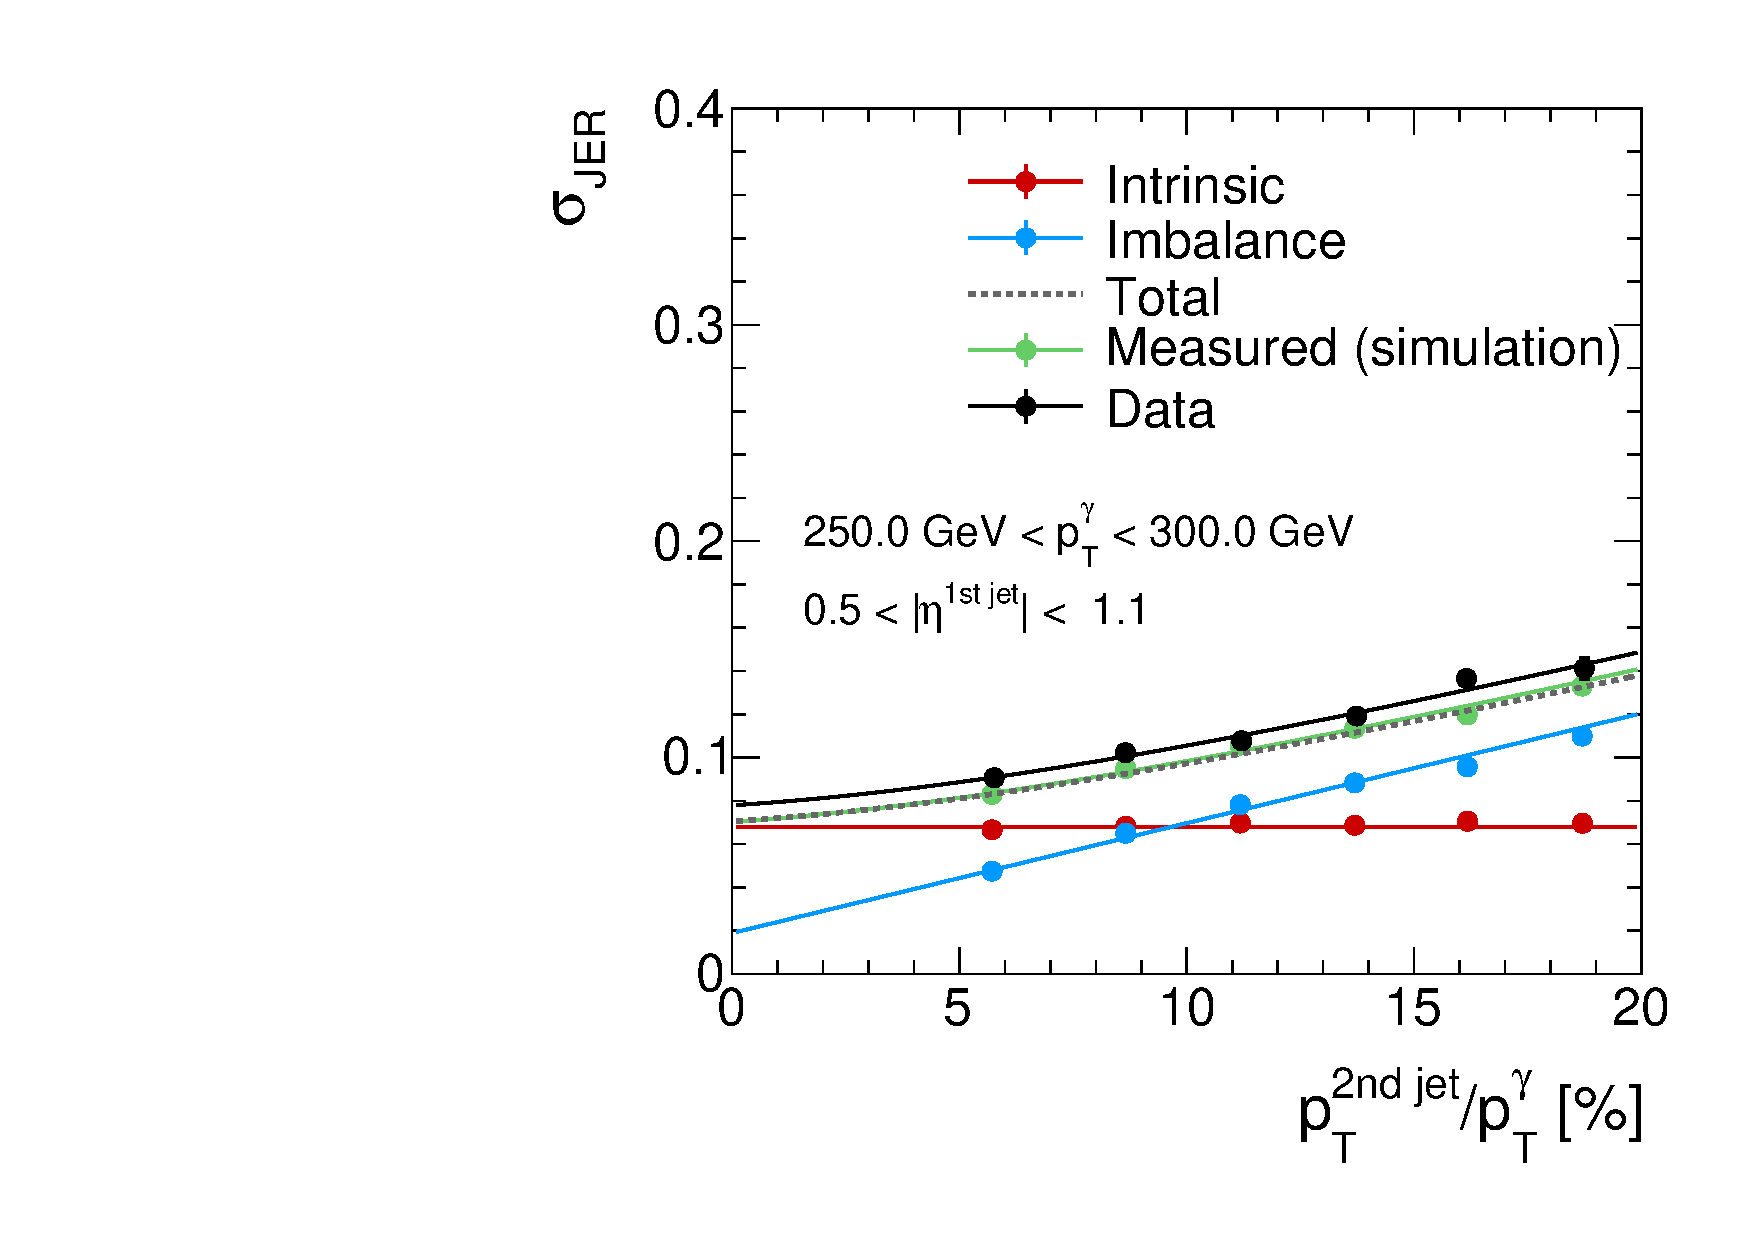
\includegraphics[width=0.32\textwidth]{figures/resolution/results/JER_for_2_eta_bin_10_pTGamma_bin_all_contributions_PFCHS_RMS99_mc.pdf}
    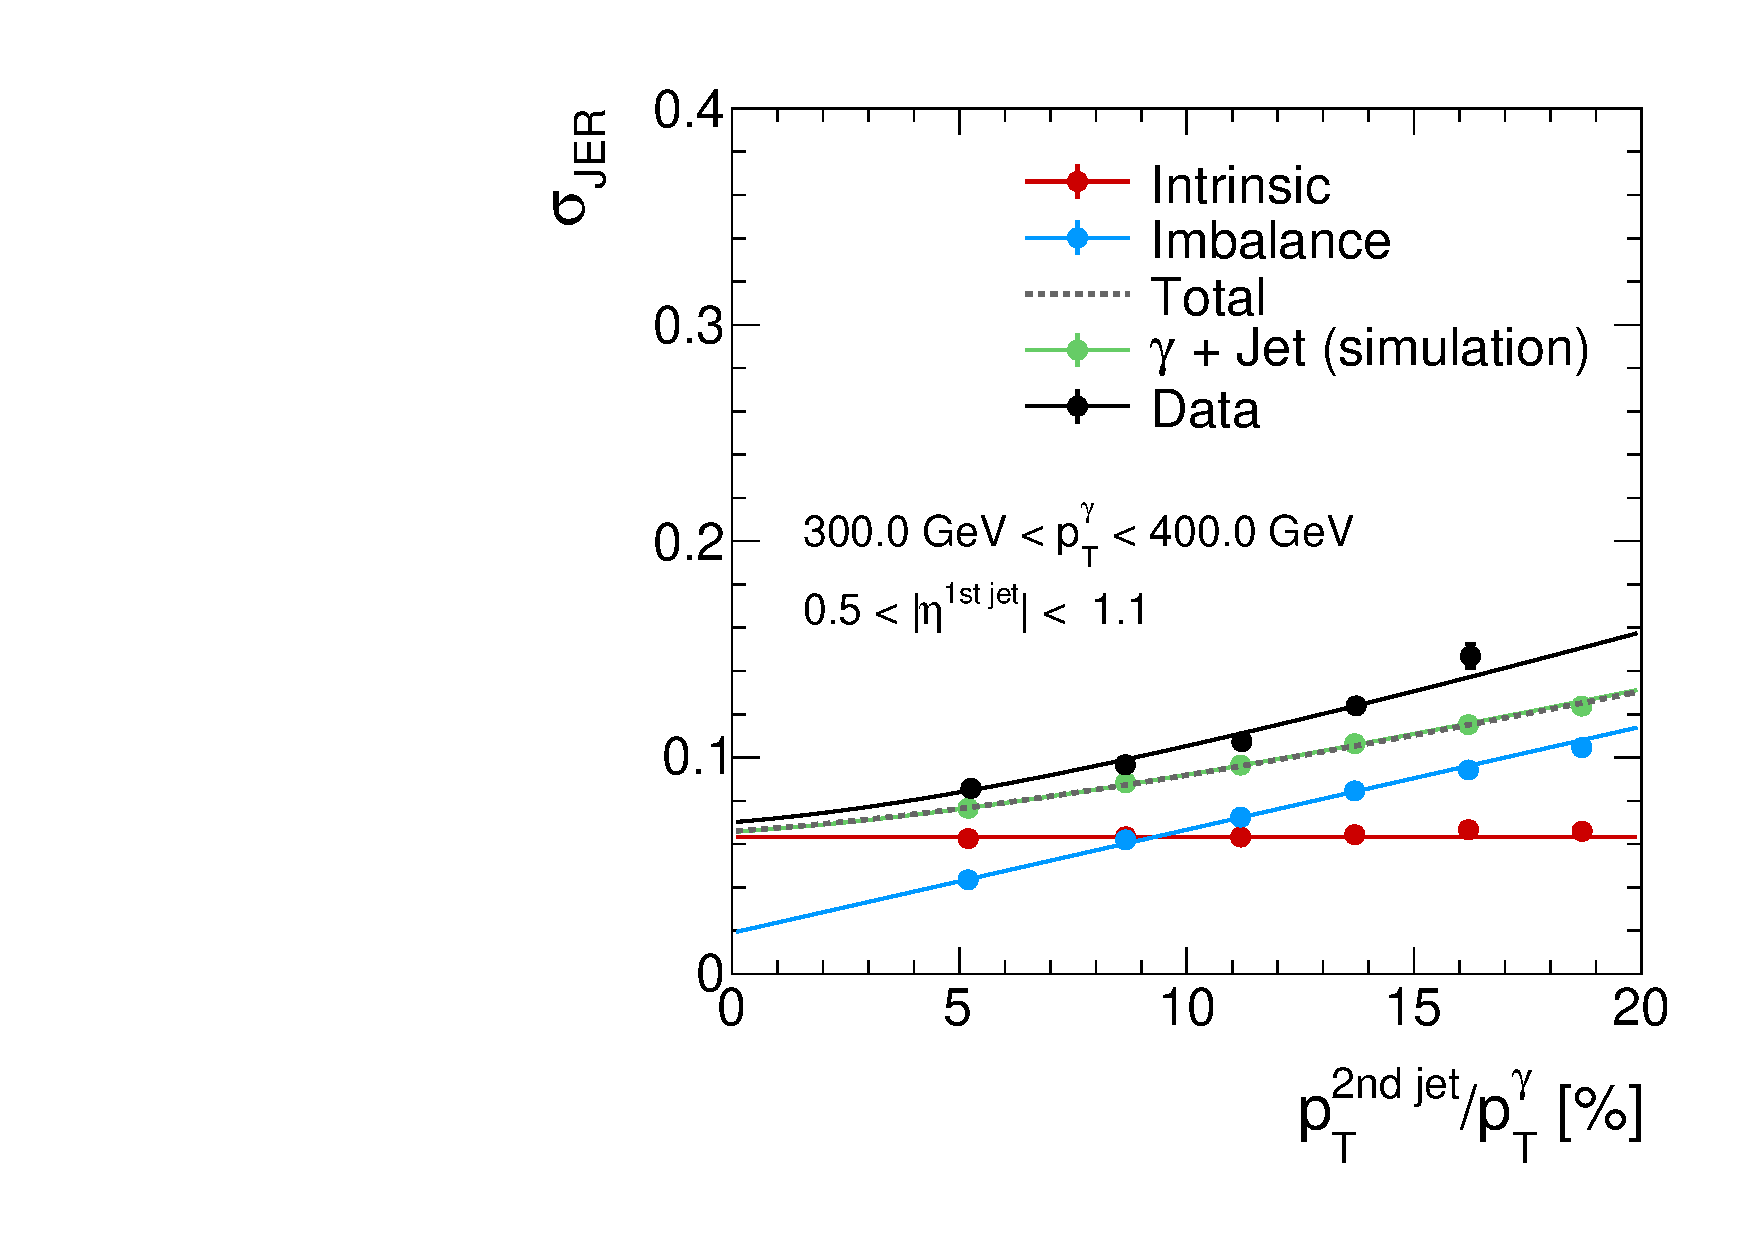
\includegraphics[width=0.32\textwidth]{figures/resolution/results/JER_for_2_eta_bin_11_pTGamma_bin_all_contributions_PFCHS_RMS99_mc.pdf}

    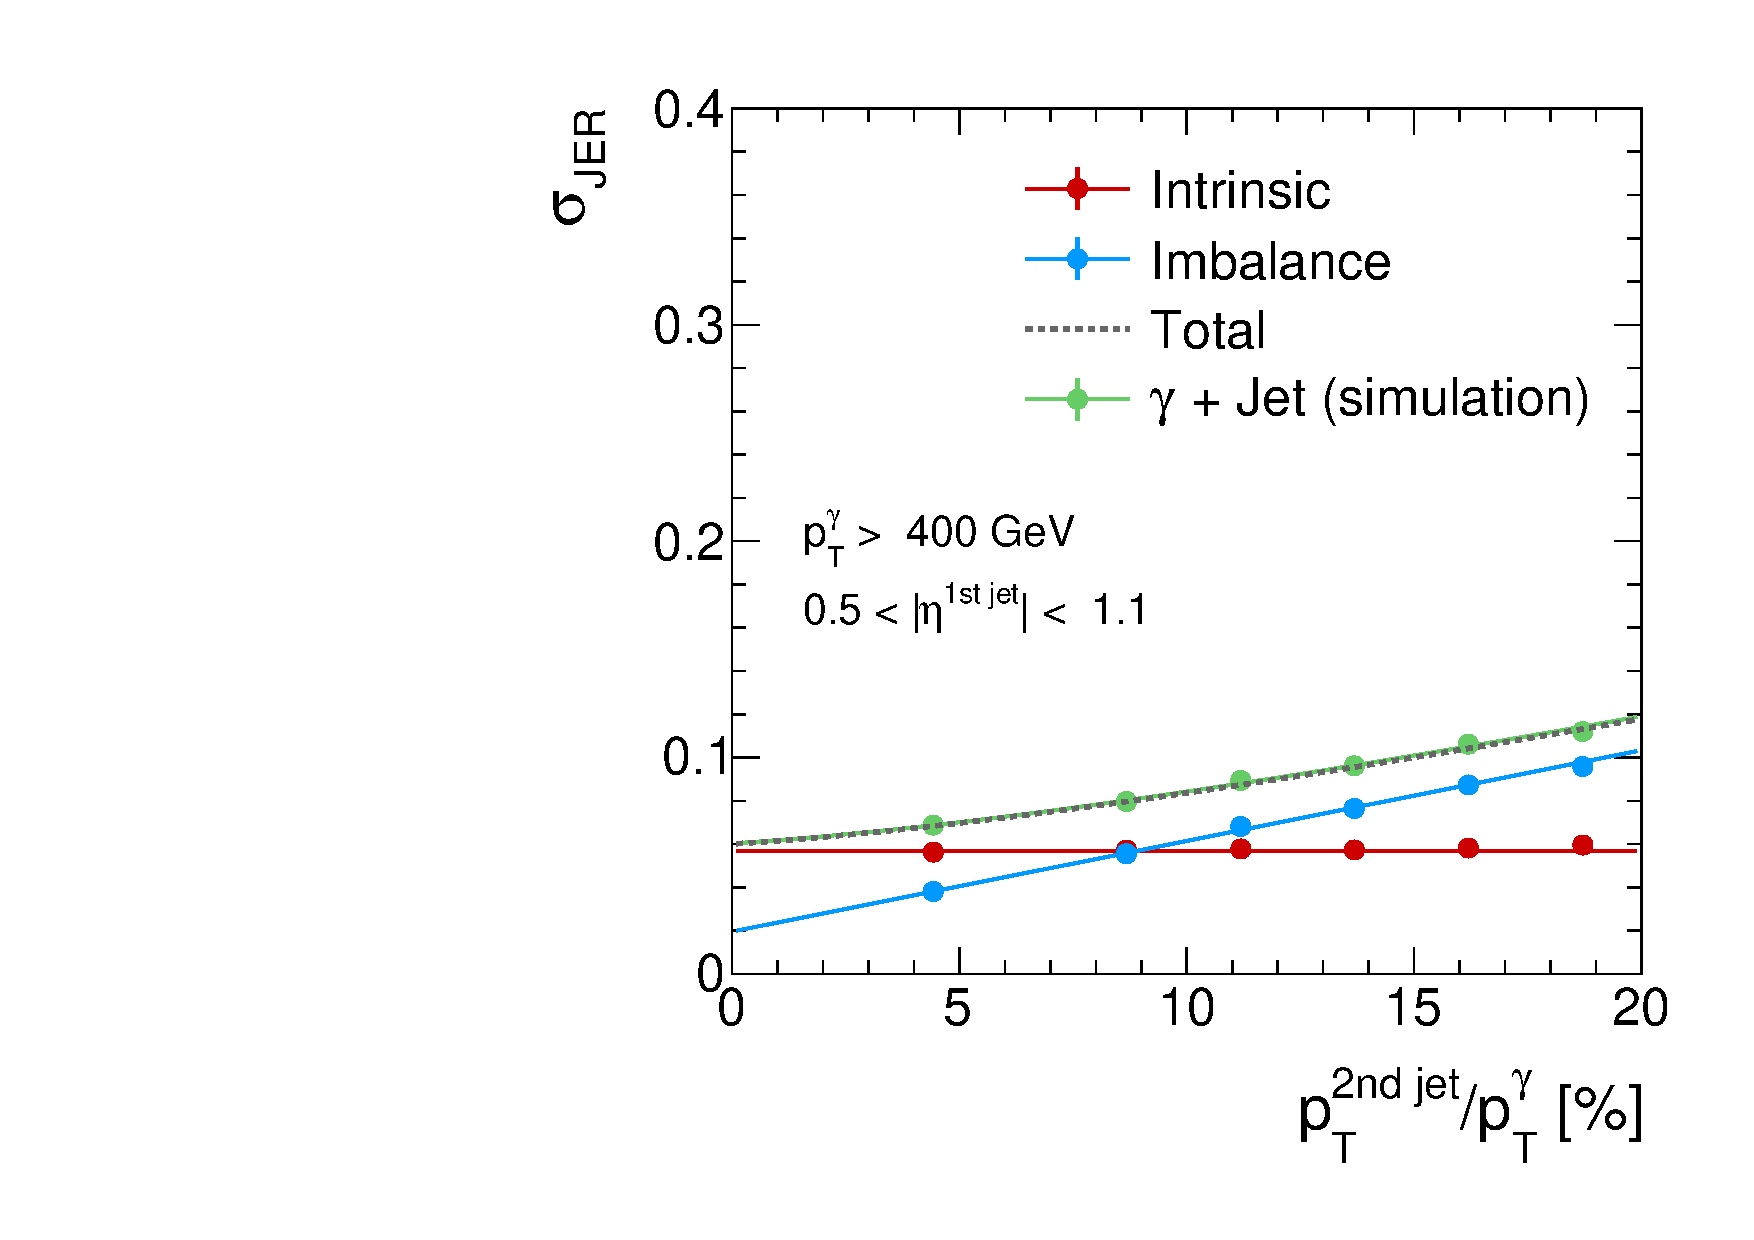
\includegraphics[width=0.32\textwidth]{figures/resolution/results/JER_for_2_eta_bin_12_pTGamma_bin_all_contributions_PFCHS_RMS99_mc.pdf}
    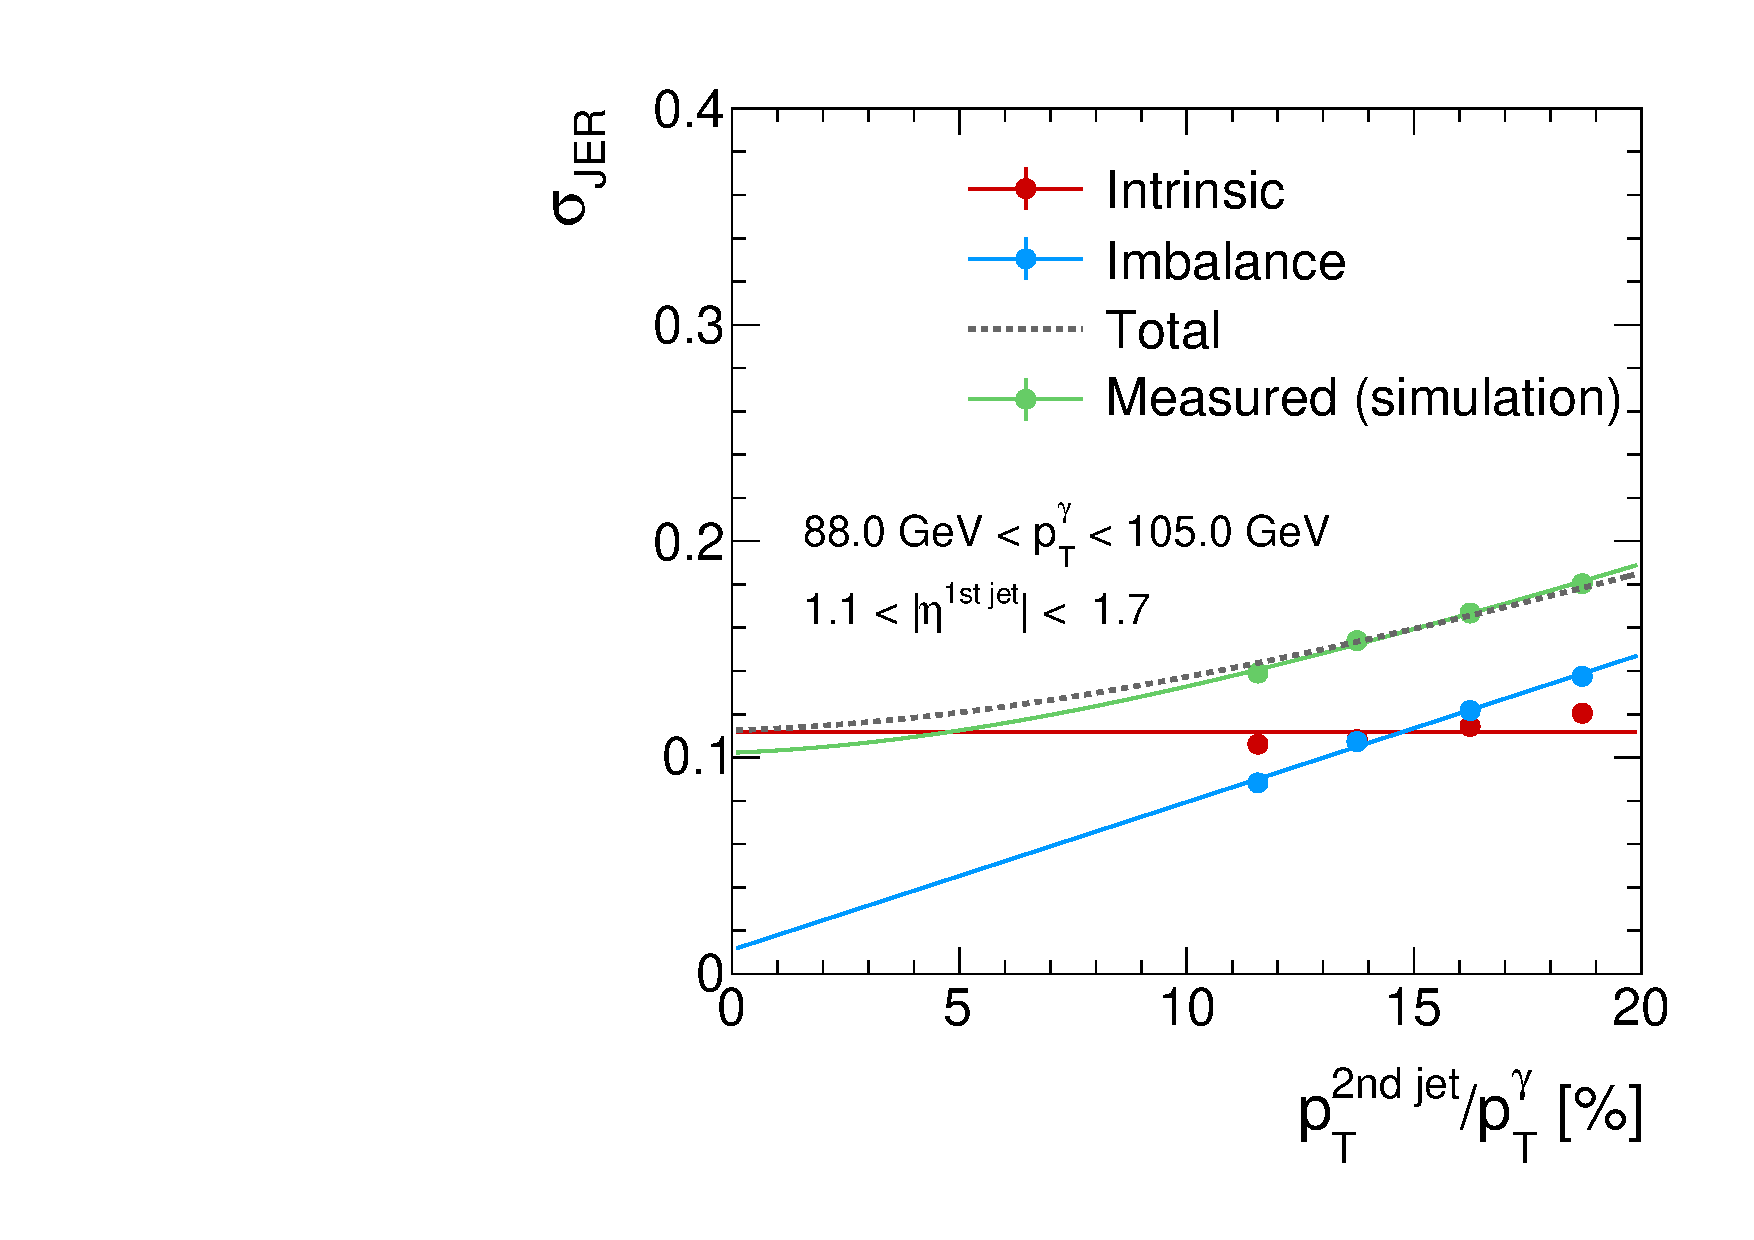
\includegraphics[width=0.32\textwidth]{figures/resolution/results/JER_for_3_eta_bin_4_pTGamma_bin_all_contributions_PFCHS_RMS99_mc.pdf}
    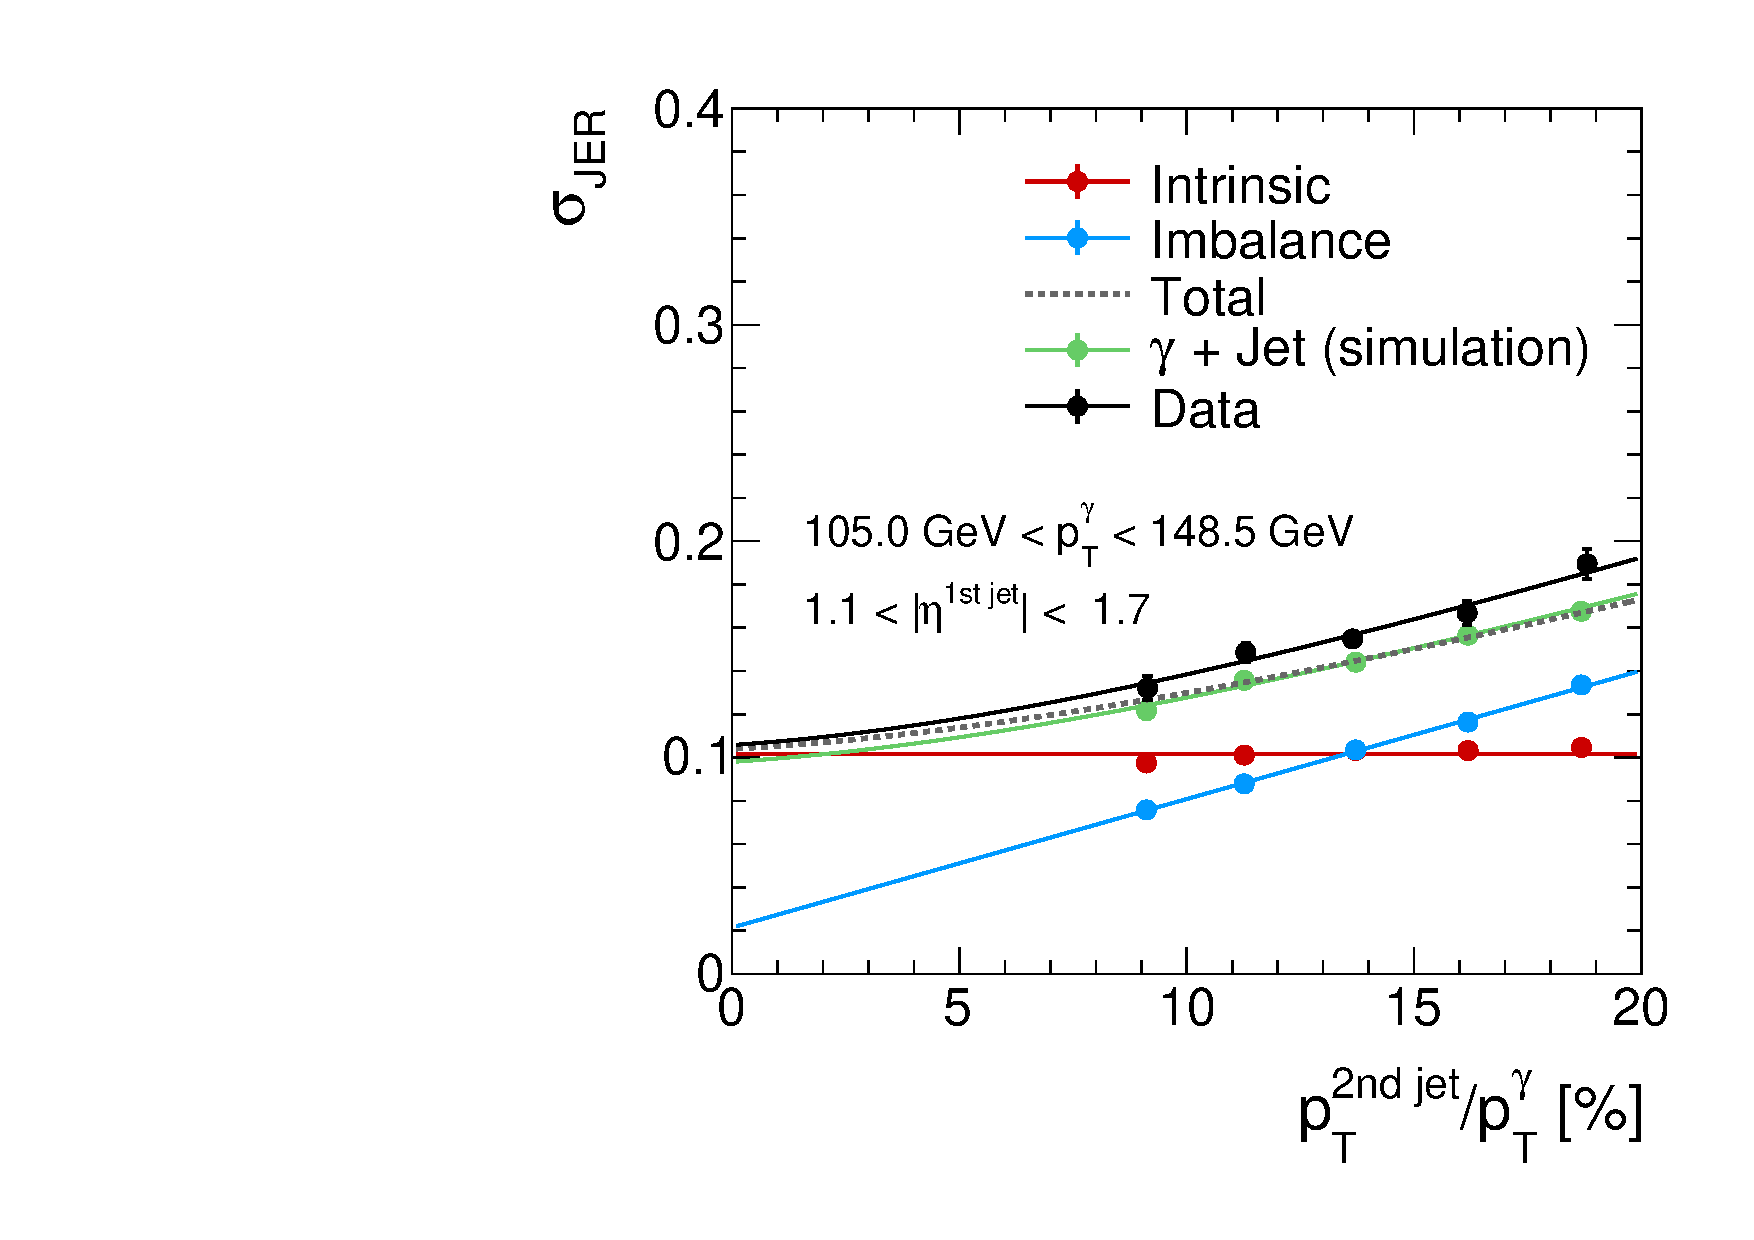
\includegraphics[width=0.32\textwidth]{figures/resolution/results/JER_for_3_eta_bin_5_pTGamma_bin_all_contributions_PFCHS_RMS99_mc.pdf}
  \caption{Continued from Fig.~\ref{fig:ExtrapolationPlots1}: \jer($\alpha$) of the intrinsic, imbalance and total resolution in simulation and the resolution measured in data for all $|\etafirstjet|$ and \ptgamma bins.}
  \label{fig:ExtrapolationPlots2}
\end{figure*}

\begin{figure*}[ht]
 \centering
    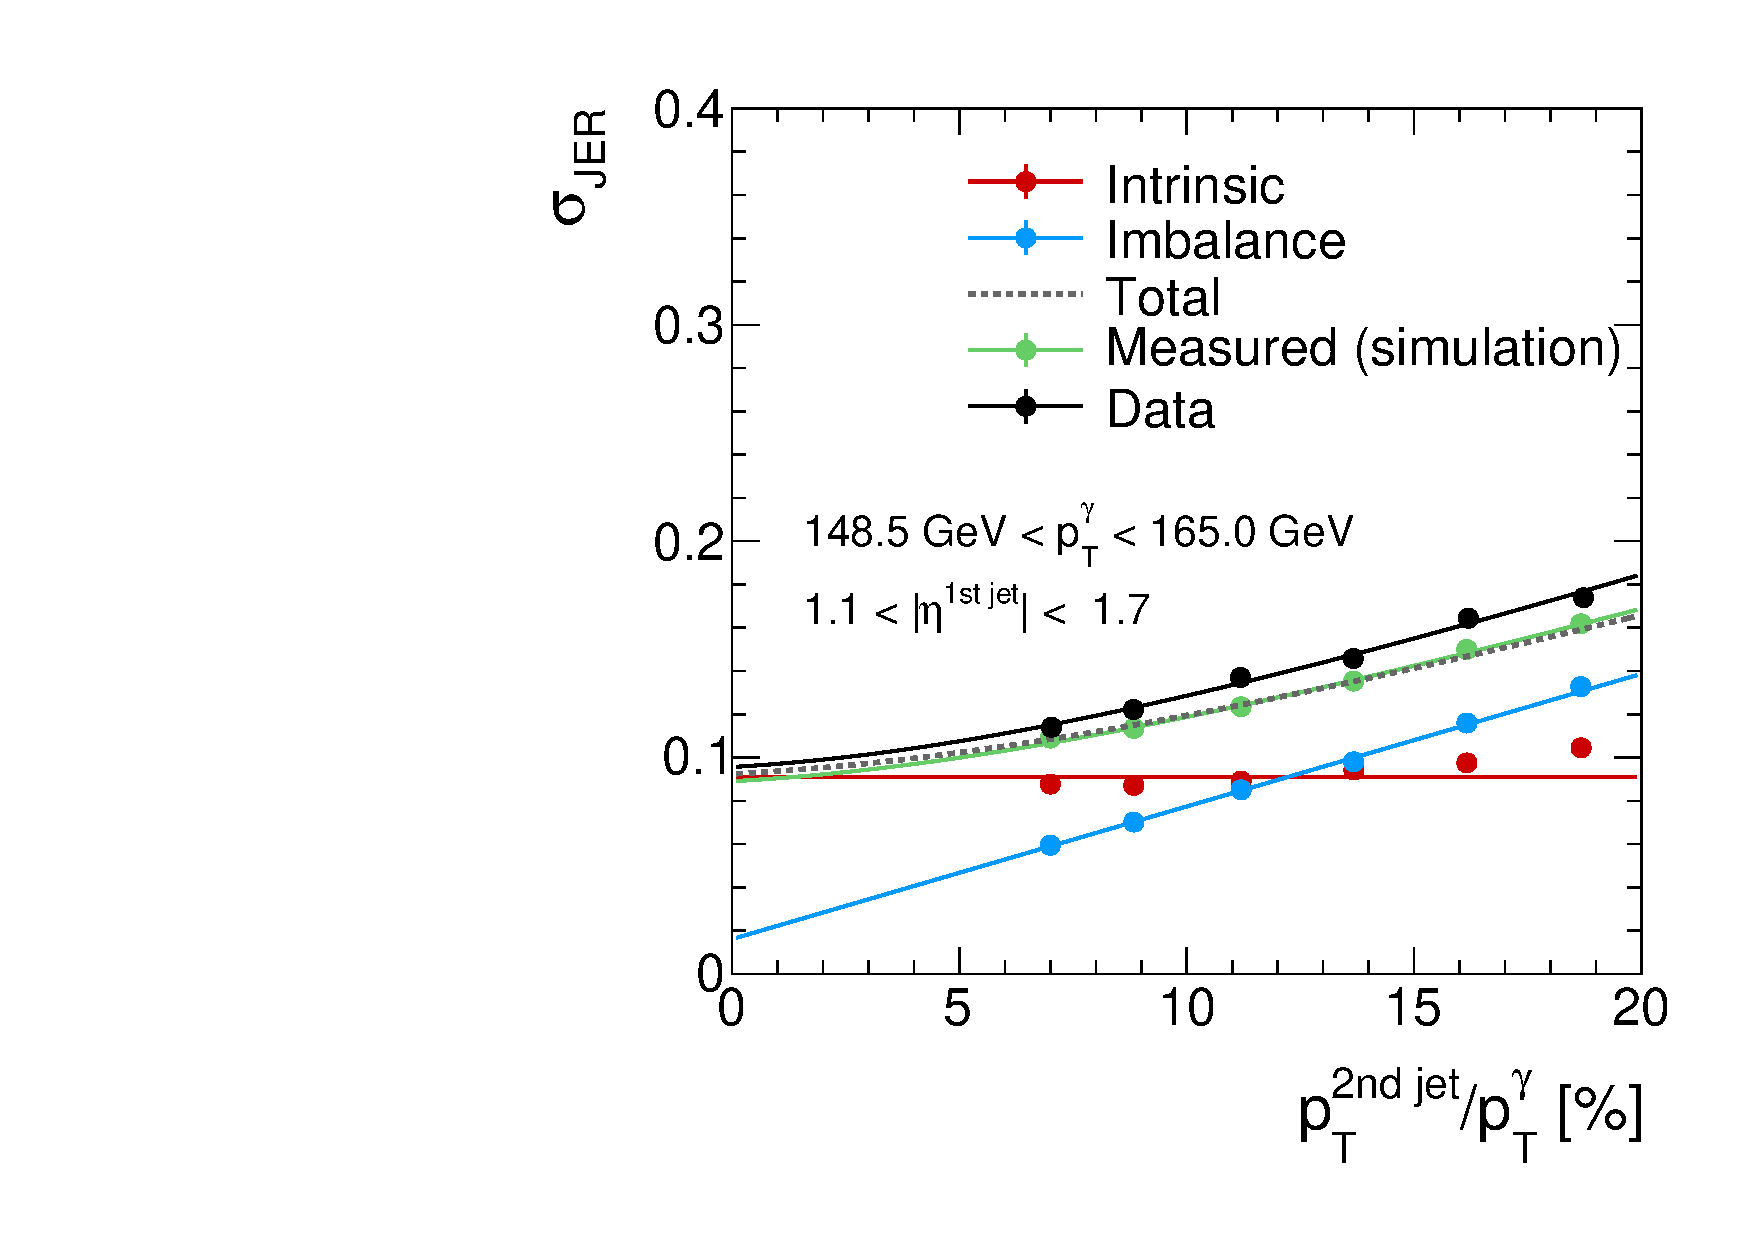
\includegraphics[width=0.32\textwidth]{figures/resolution/results/JER_for_3_eta_bin_6_pTGamma_bin_all_contributions_PFCHS_RMS99_mc.pdf}
    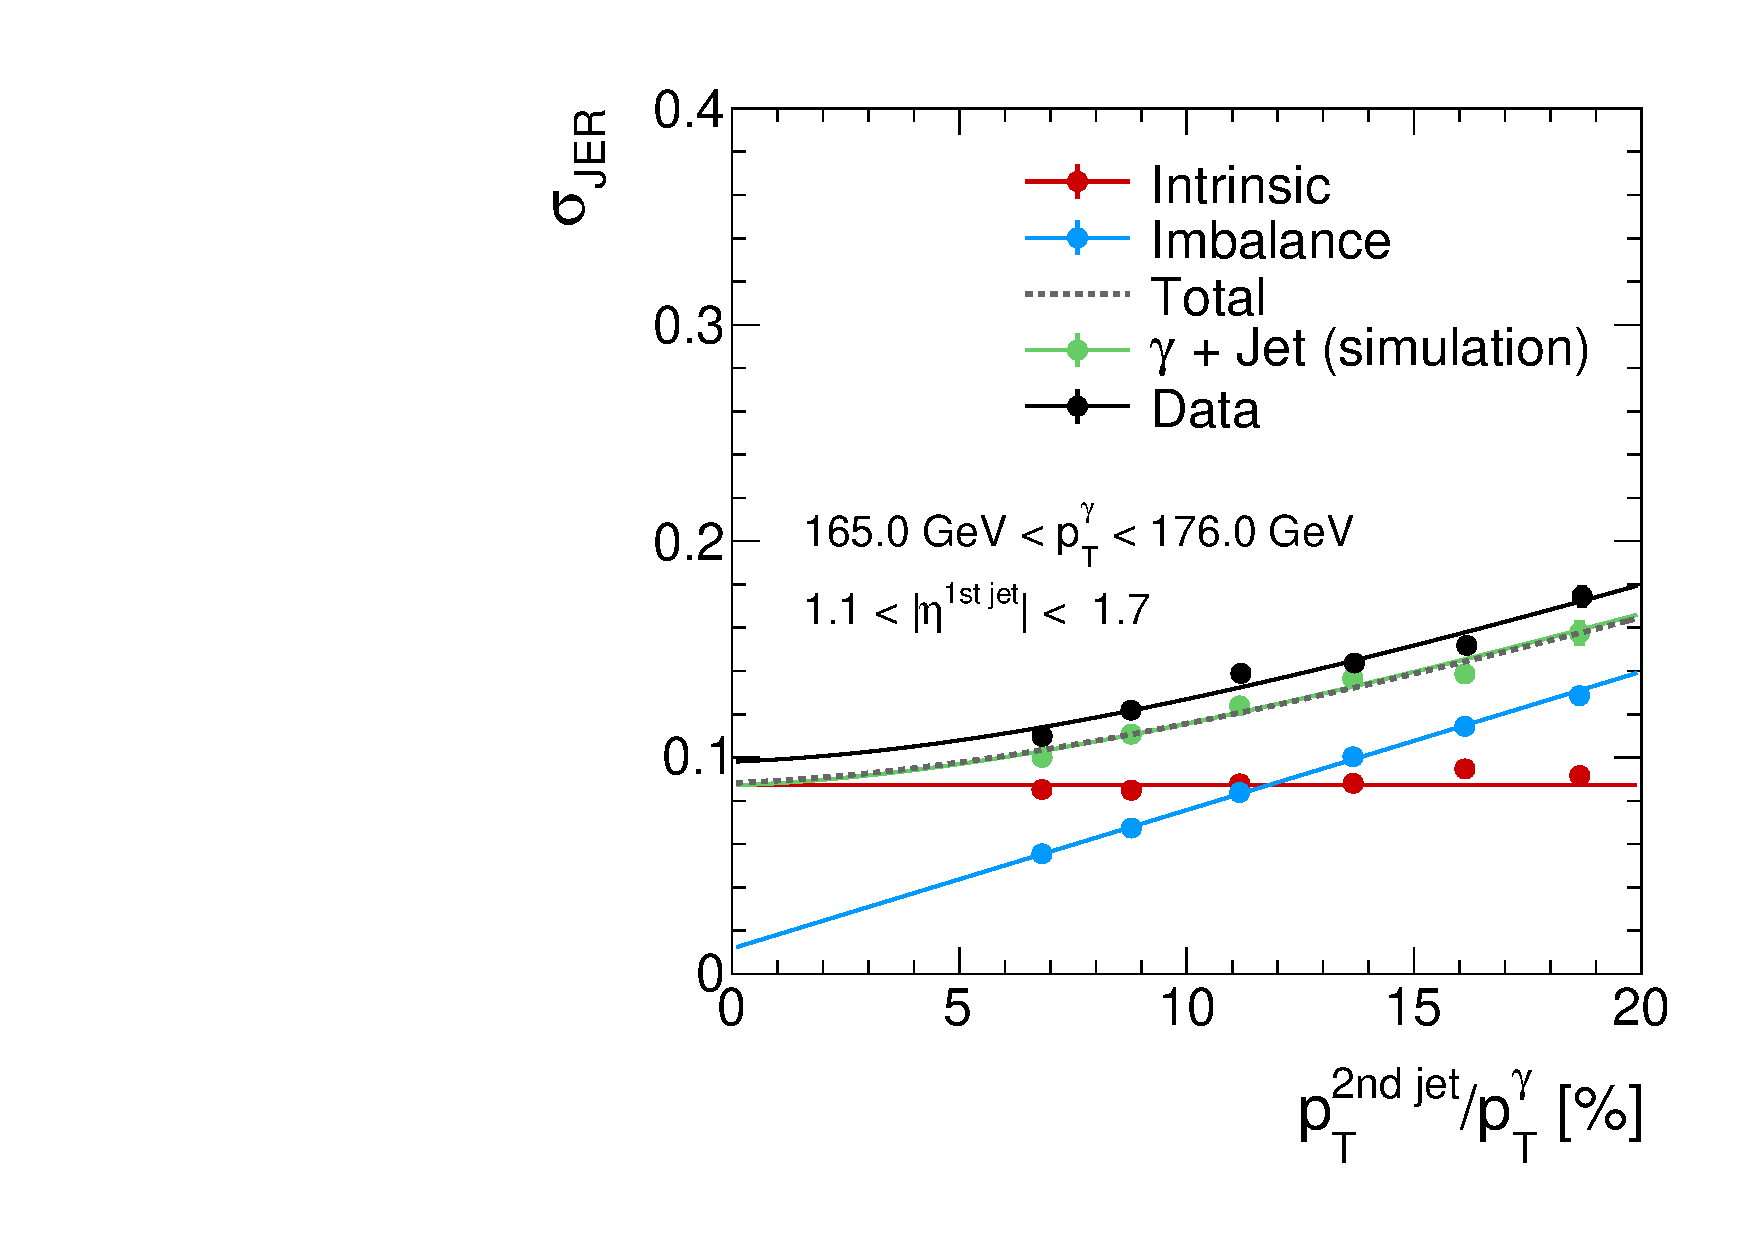
\includegraphics[width=0.32\textwidth]{figures/resolution/results/JER_for_3_eta_bin_7_pTGamma_bin_all_contributions_PFCHS_RMS99_mc.pdf}
    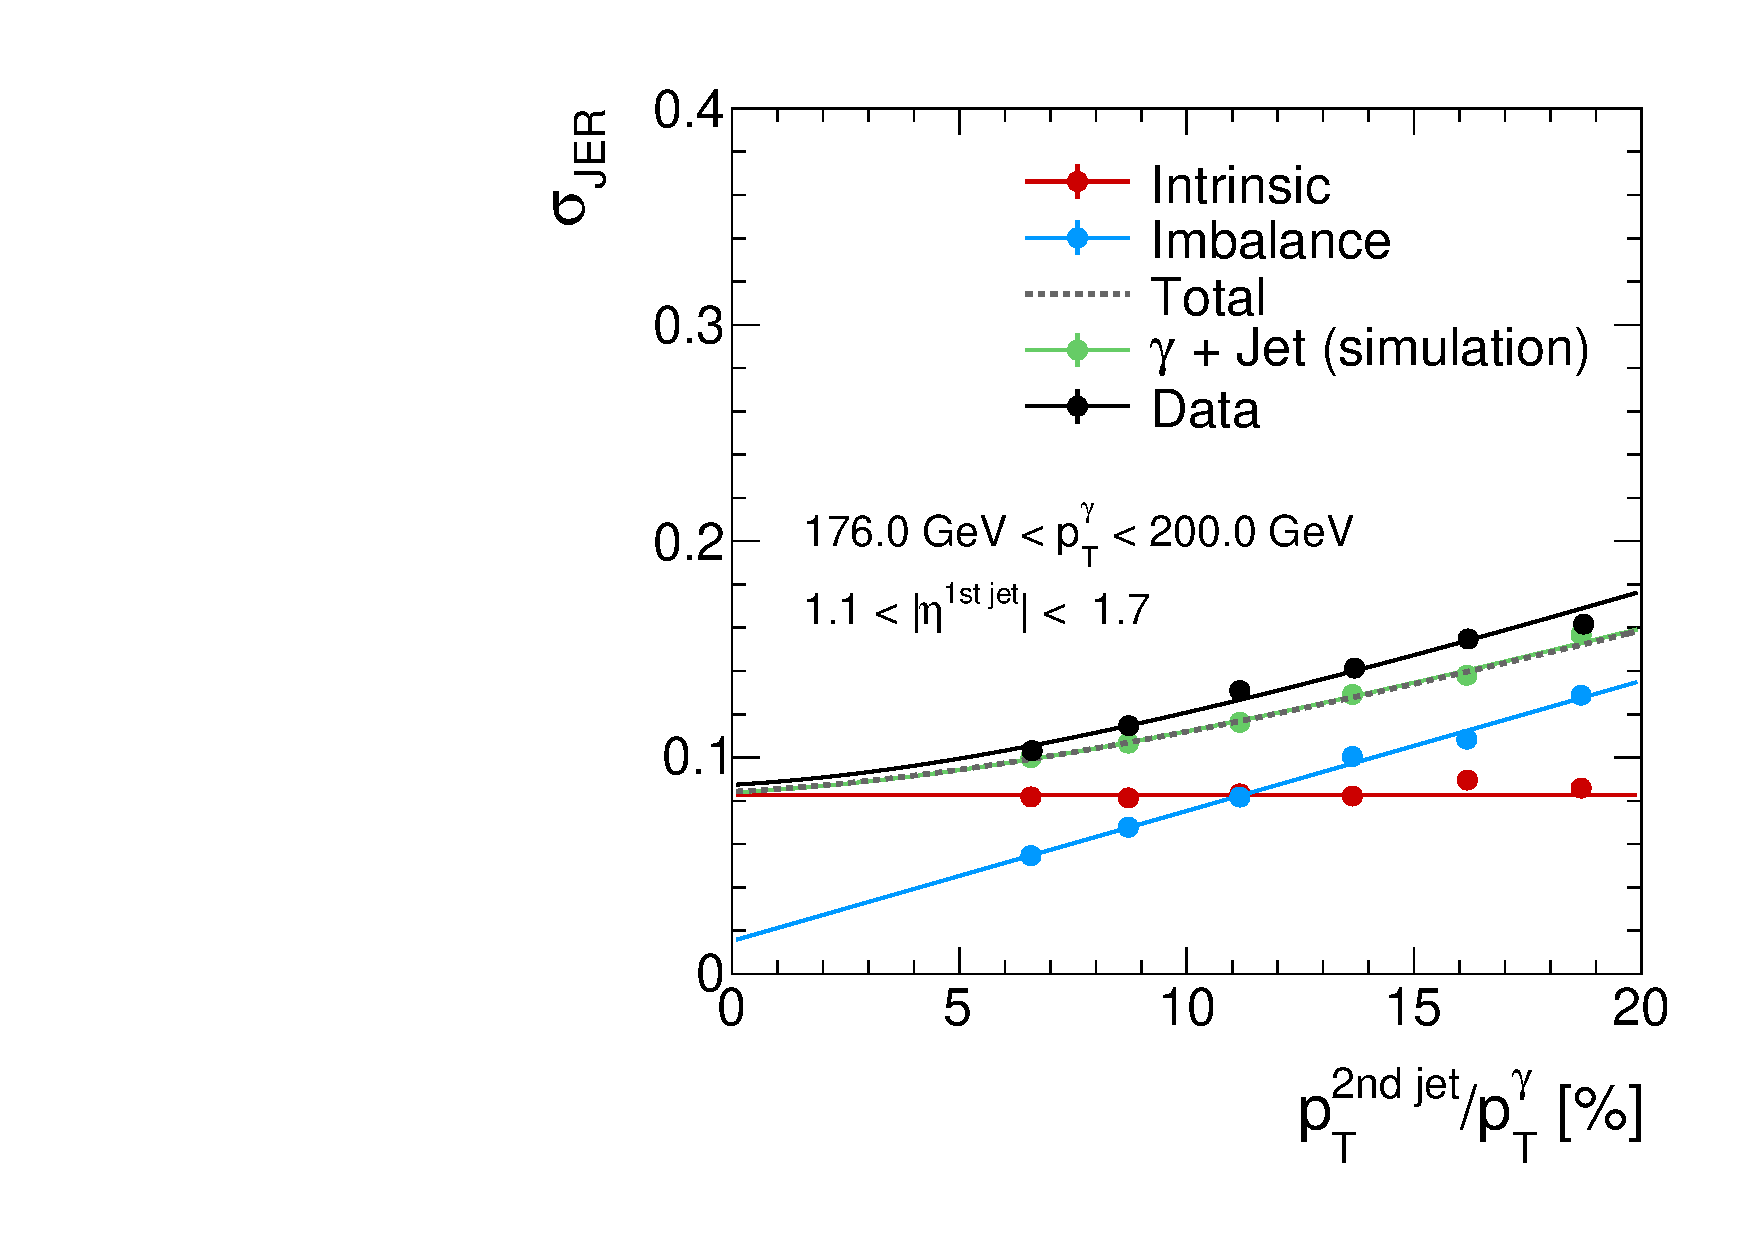
\includegraphics[width=0.32\textwidth]{figures/resolution/results/JER_for_3_eta_bin_8_pTGamma_bin_all_contributions_PFCHS_RMS99_mc.pdf}

    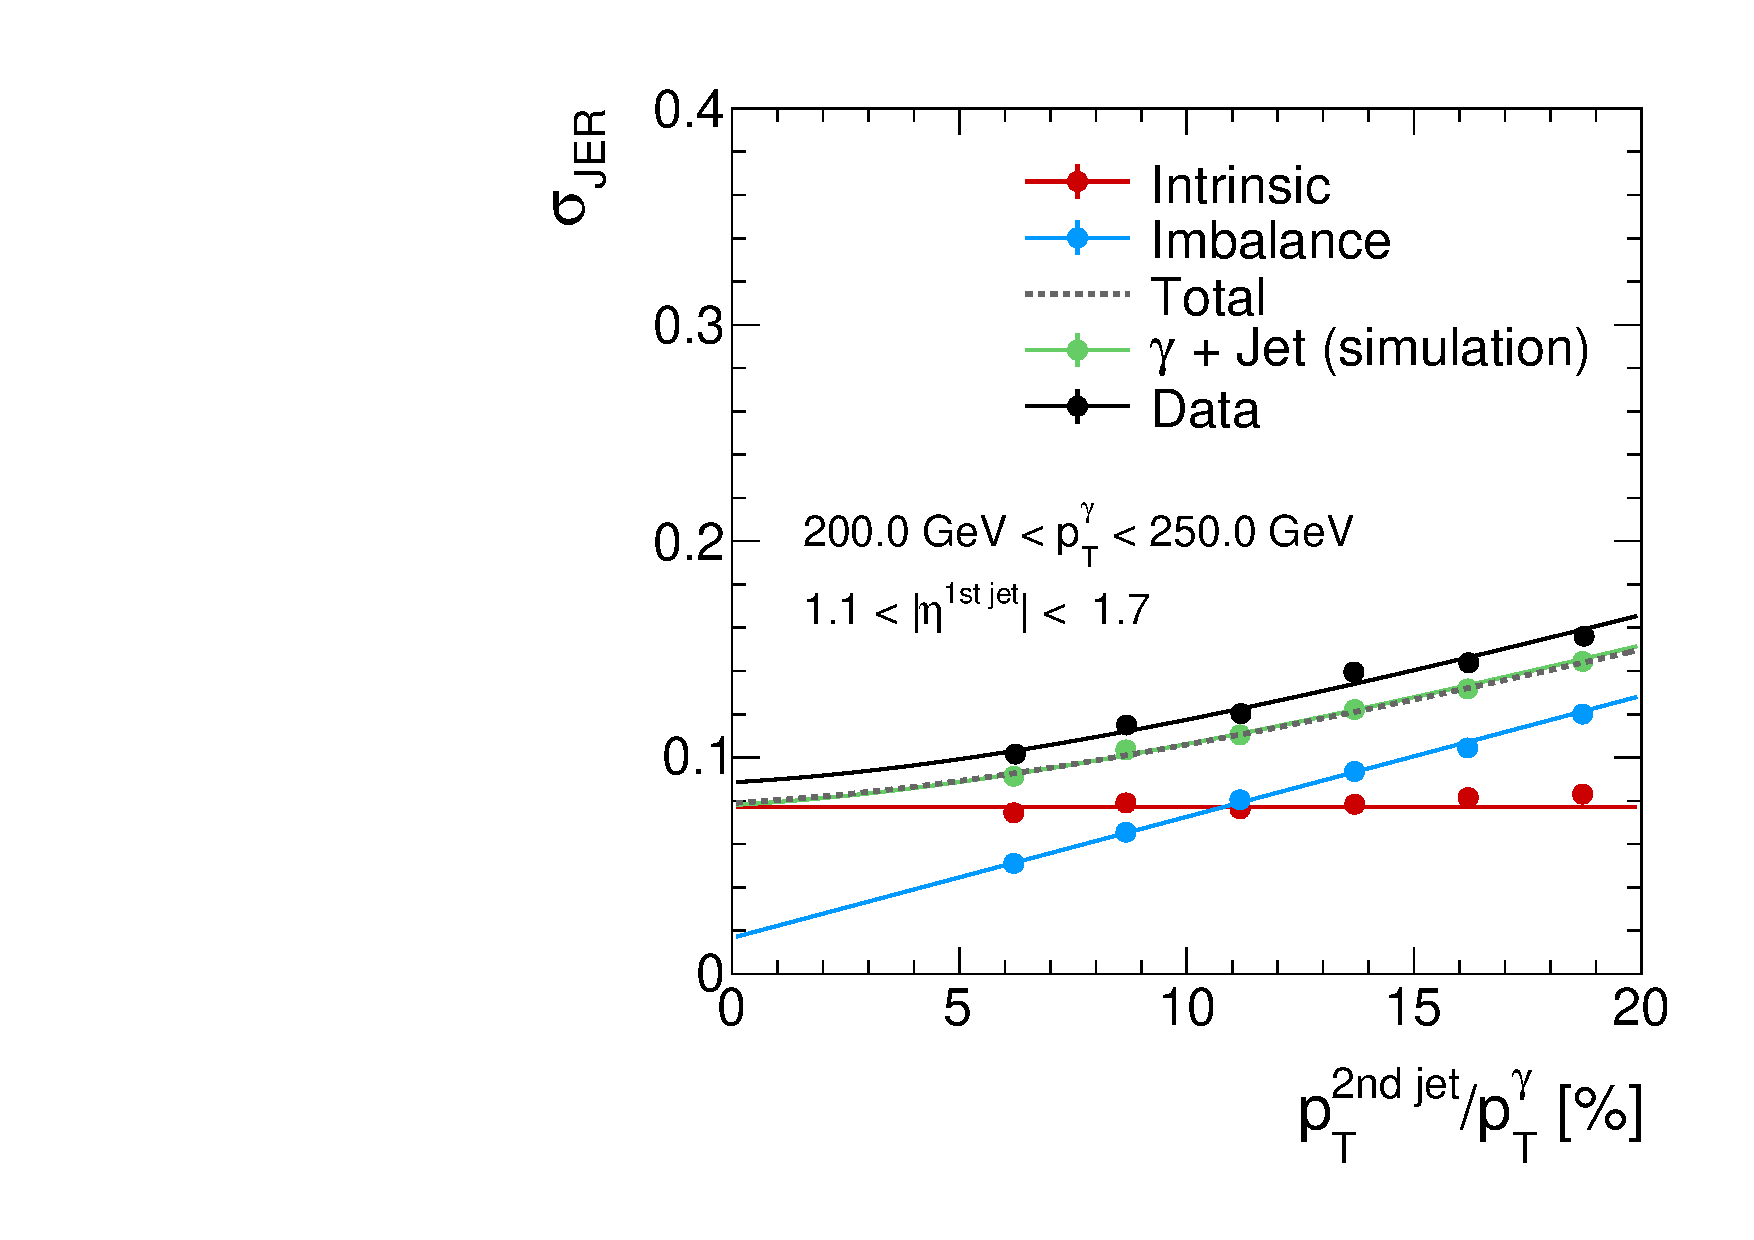
\includegraphics[width=0.32\textwidth]{figures/resolution/results/JER_for_3_eta_bin_9_pTGamma_bin_all_contributions_PFCHS_RMS99_mc.pdf}
    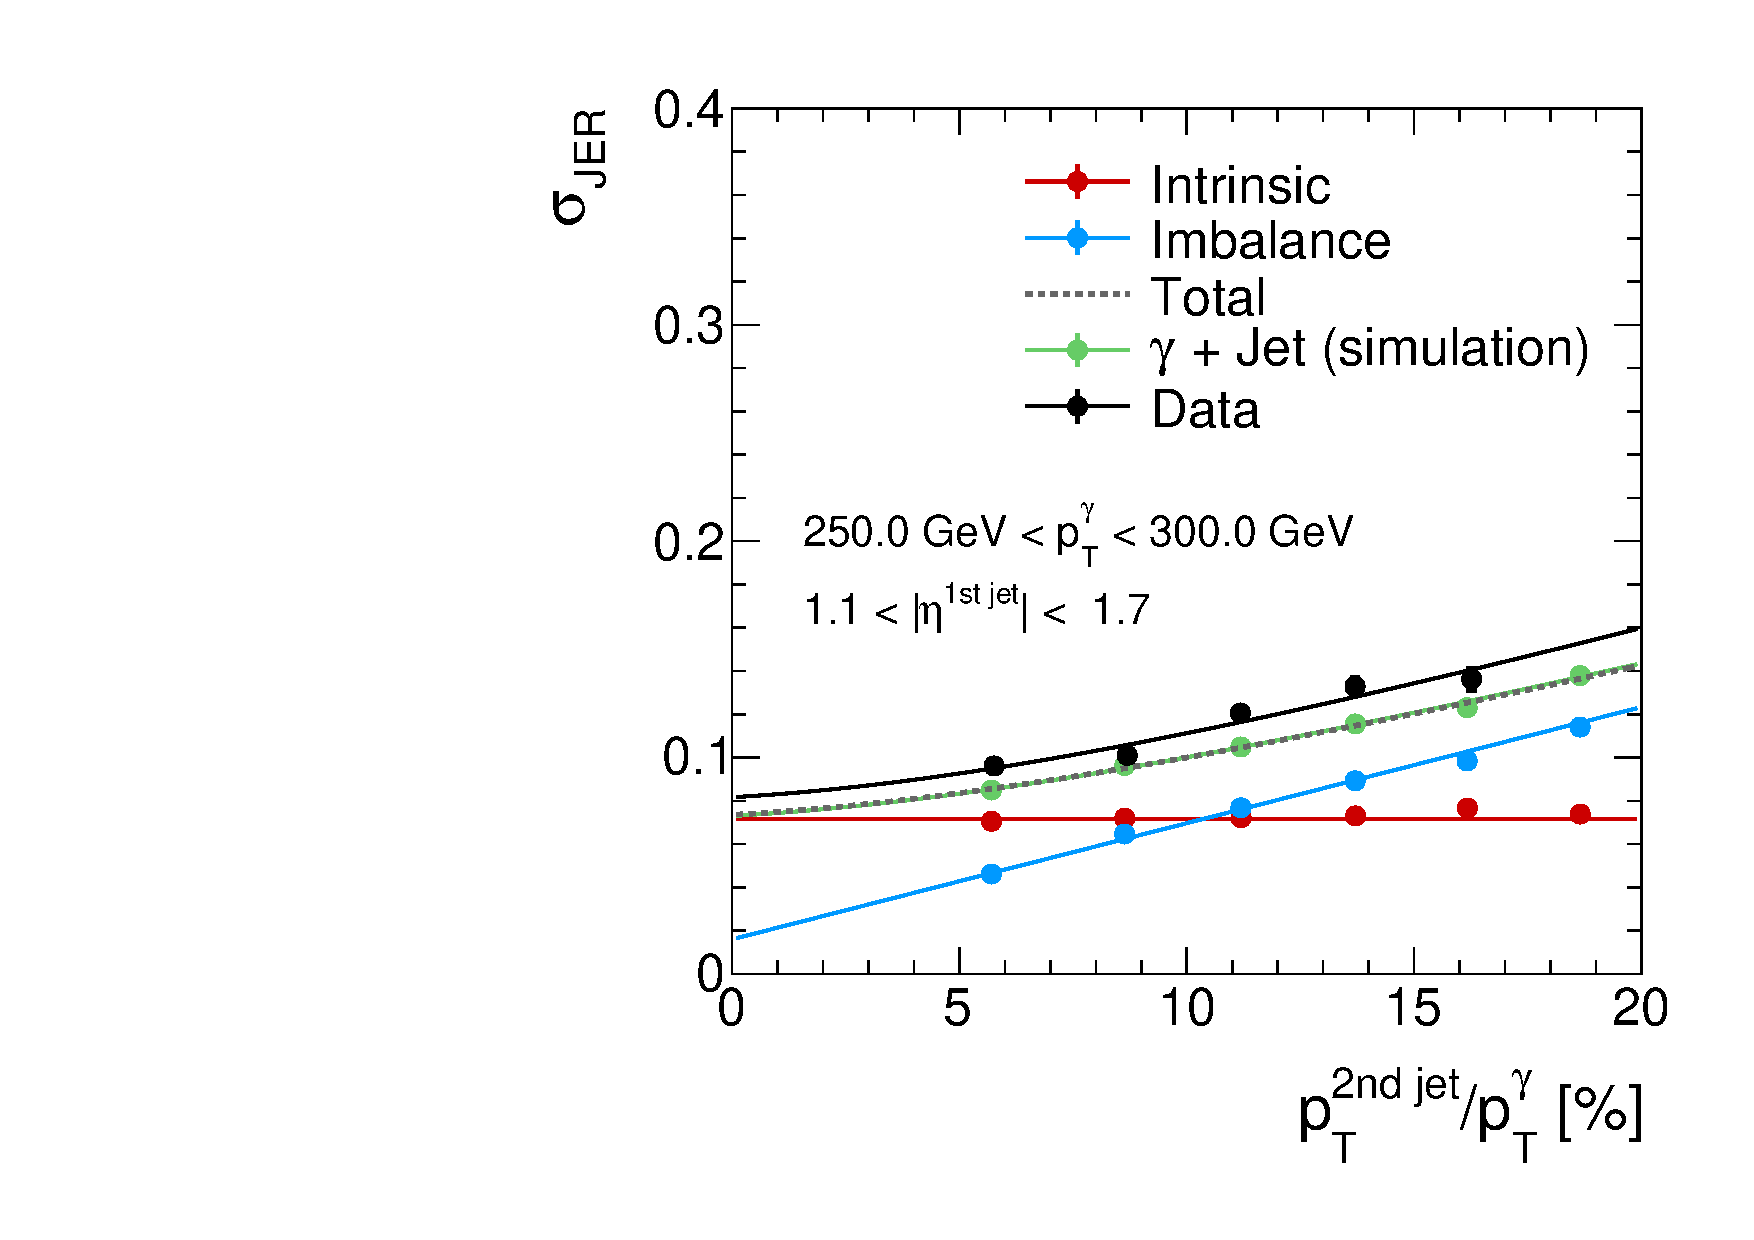
\includegraphics[width=0.32\textwidth]{figures/resolution/results/JER_for_3_eta_bin_10_pTGamma_bin_all_contributions_PFCHS_RMS99_mc.pdf}
    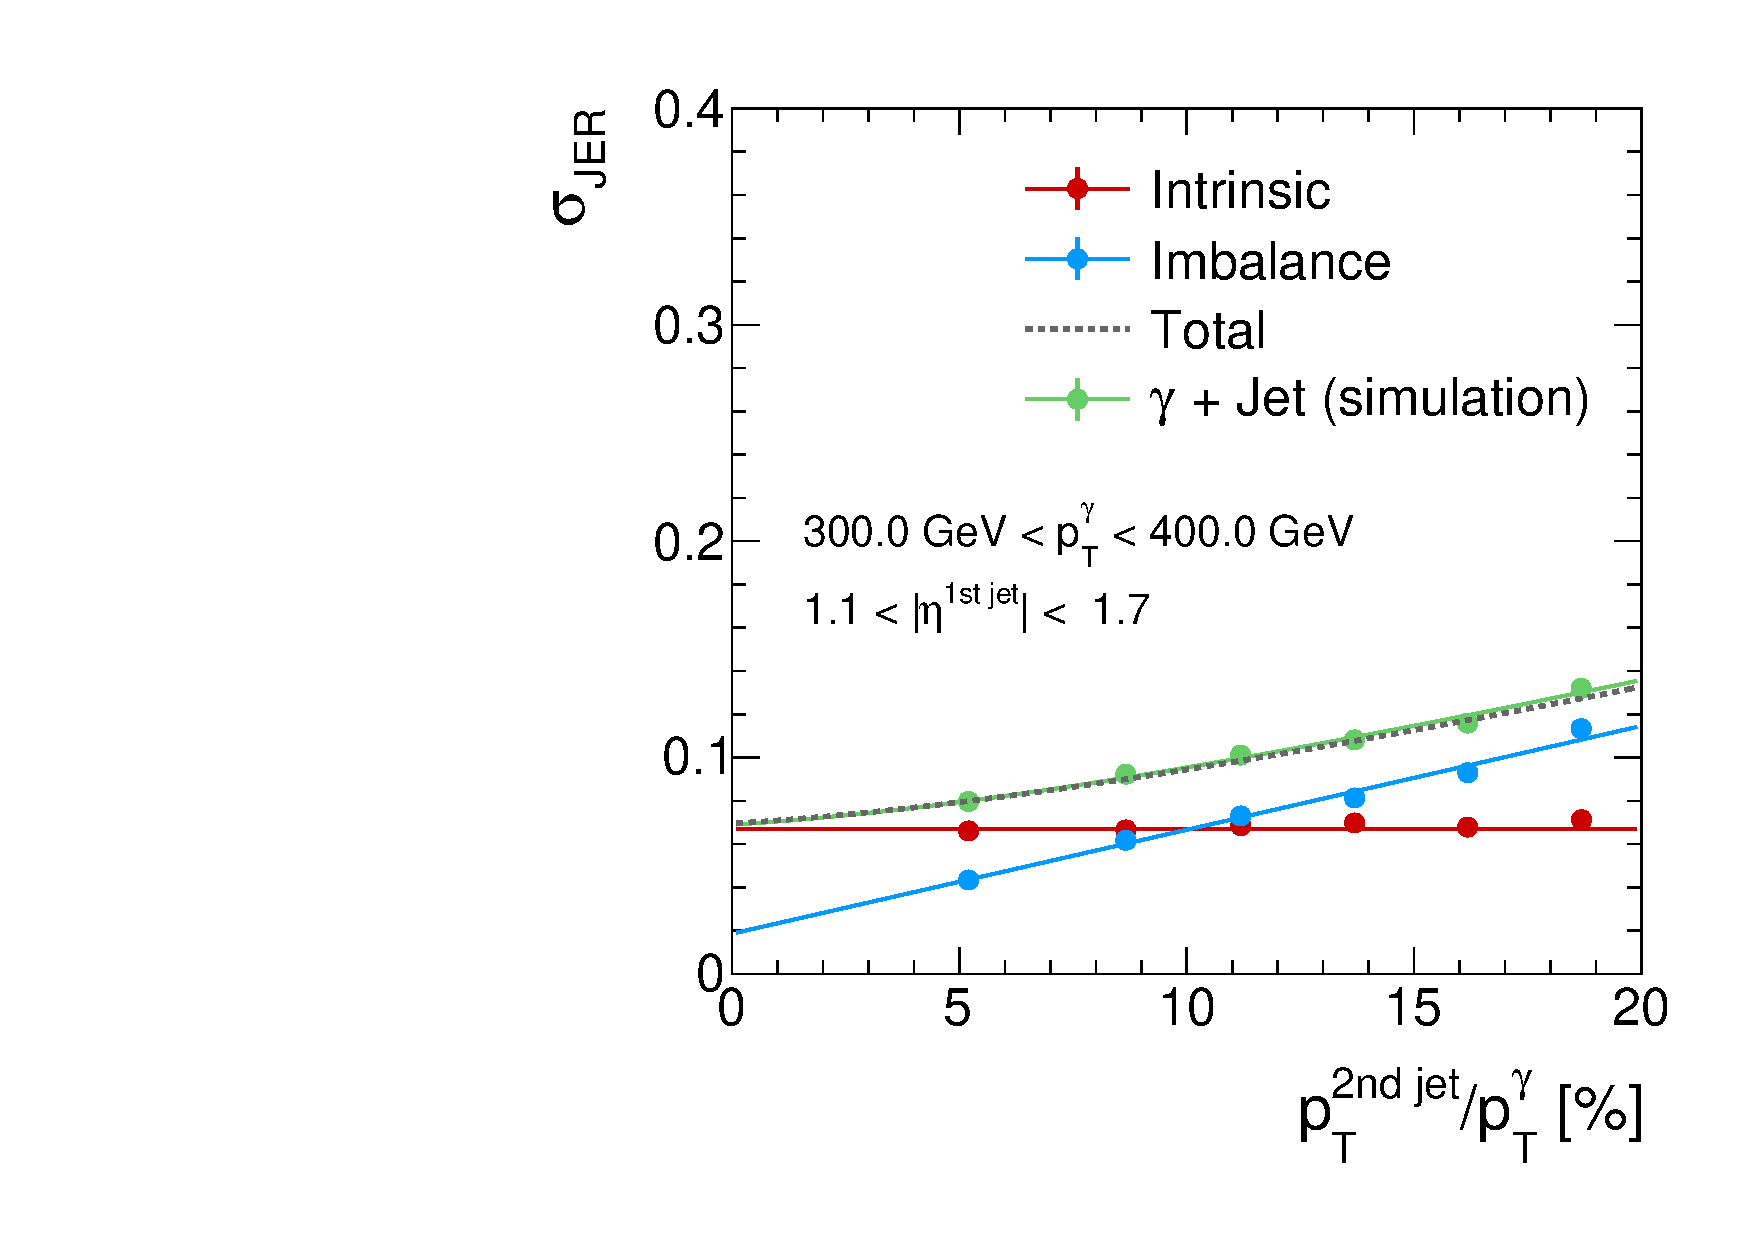
\includegraphics[width=0.32\textwidth]{figures/resolution/results/JER_for_3_eta_bin_11_pTGamma_bin_all_contributions_PFCHS_RMS99_mc.pdf}

    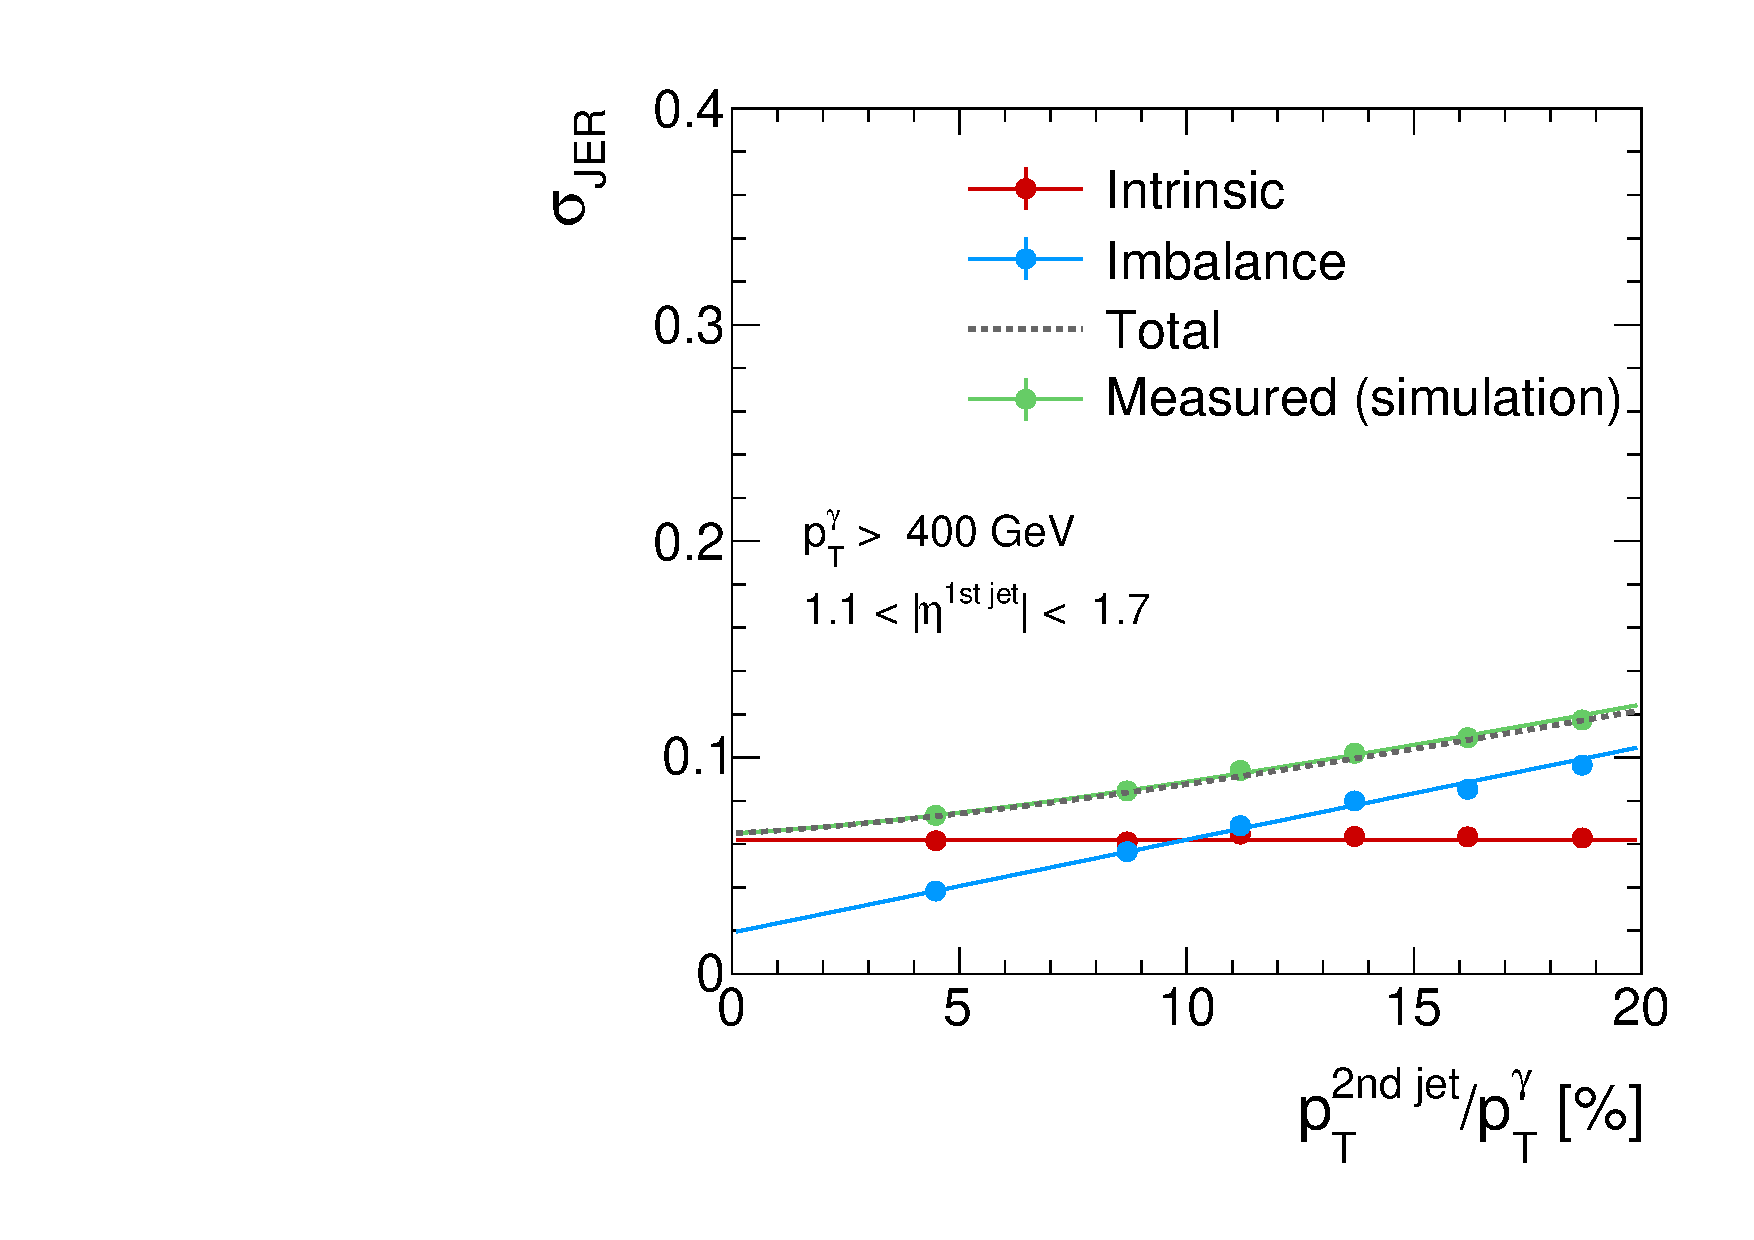
\includegraphics[width=0.32\textwidth]{figures/resolution/results/JER_for_3_eta_bin_12_pTGamma_bin_all_contributions_PFCHS_RMS99_mc.pdf}
    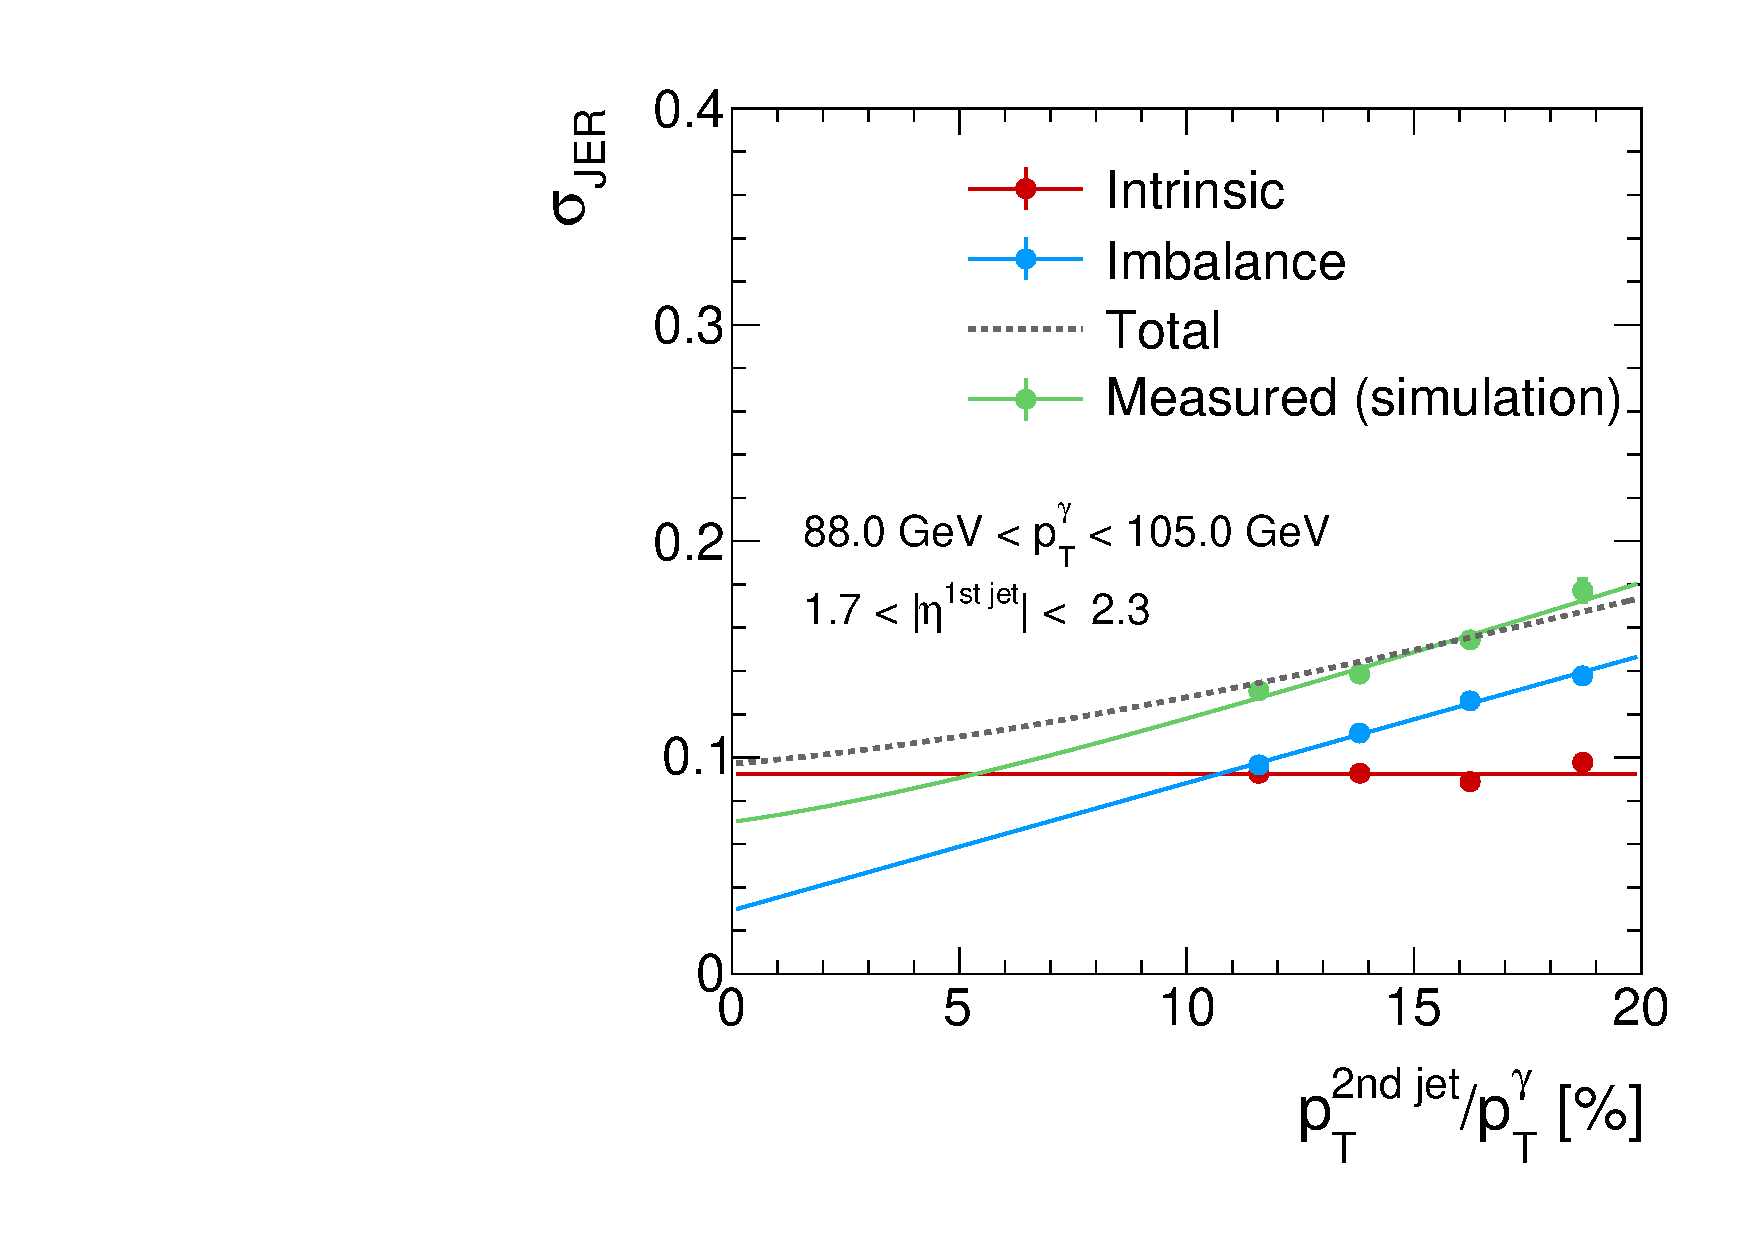
\includegraphics[width=0.32\textwidth]{figures/resolution/results/JER_for_4_eta_bin_4_pTGamma_bin_all_contributions_PFCHS_RMS99_mc.pdf}
    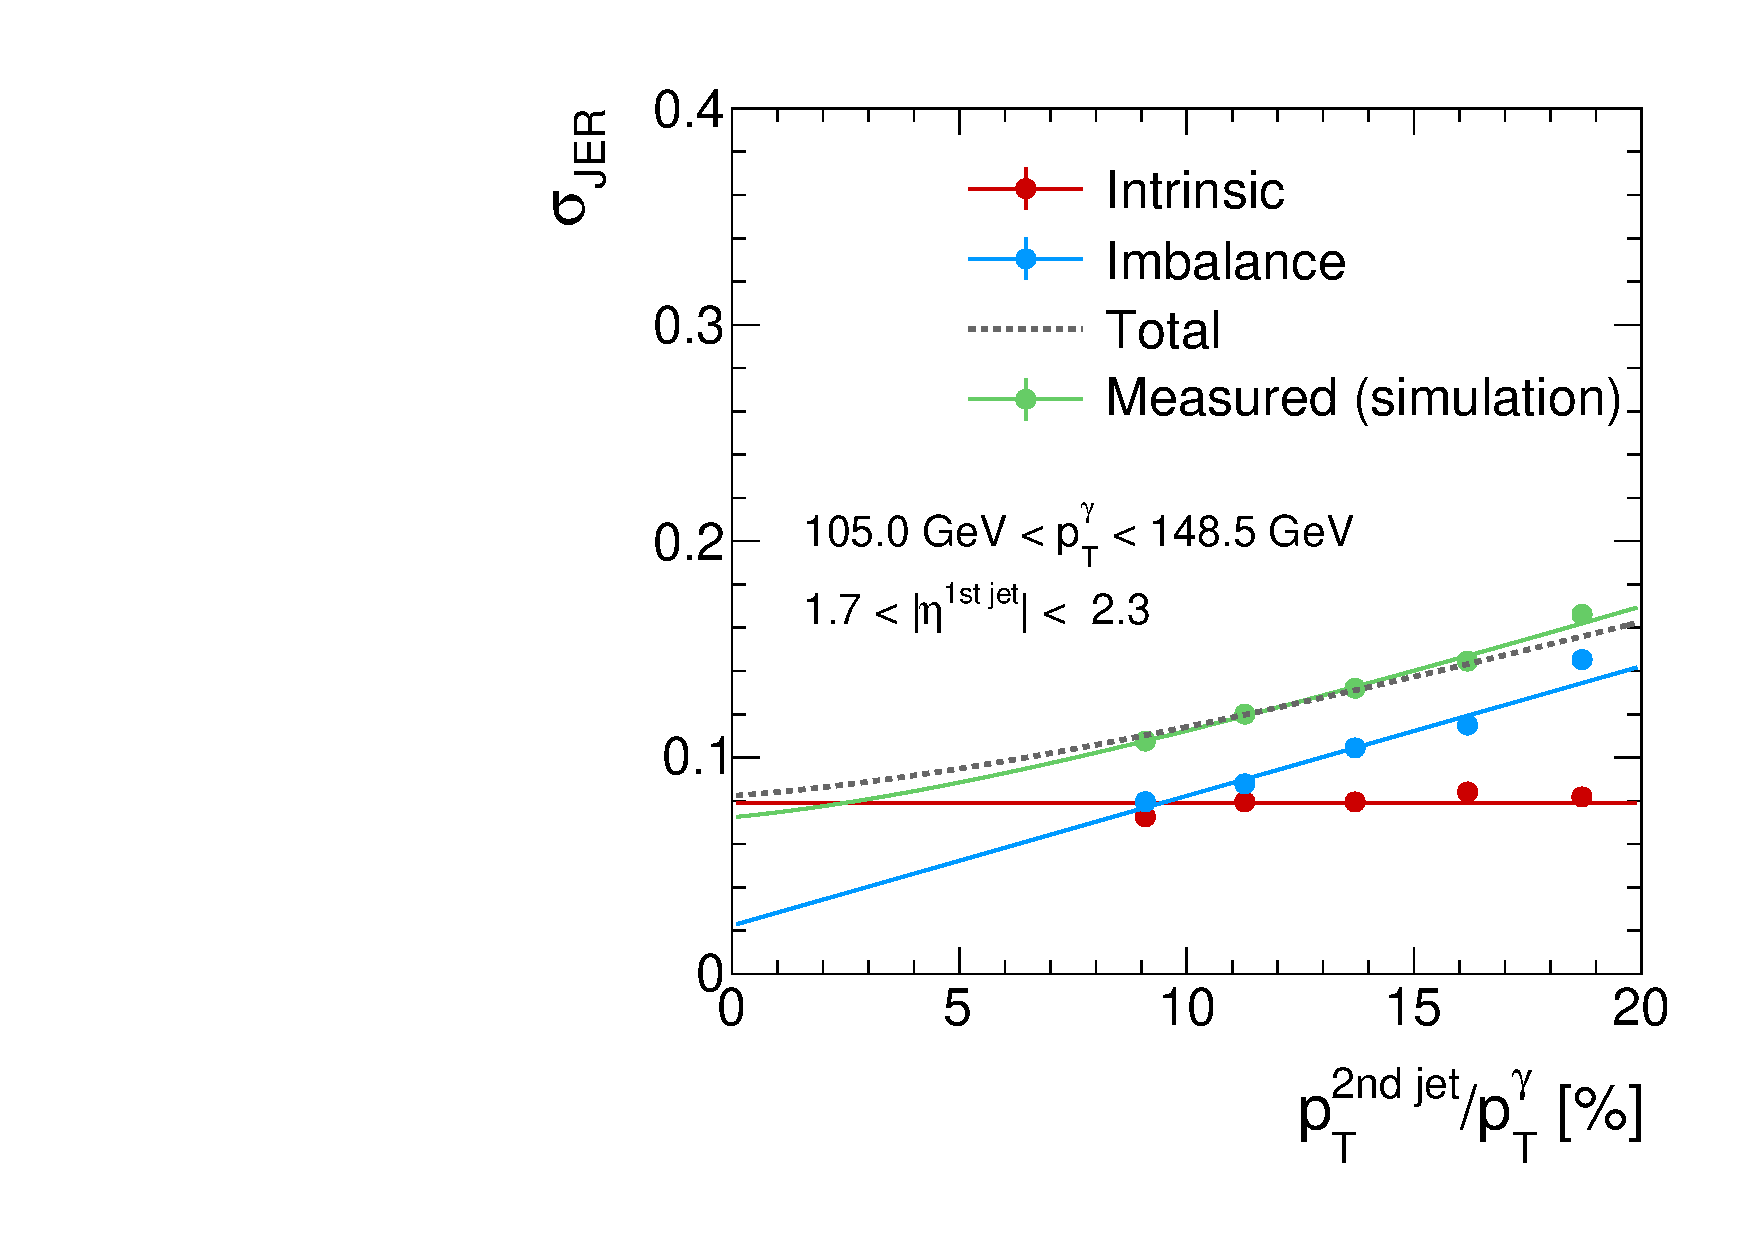
\includegraphics[width=0.32\textwidth]{figures/resolution/results/JER_for_4_eta_bin_5_pTGamma_bin_all_contributions_PFCHS_RMS99_mc.pdf}

    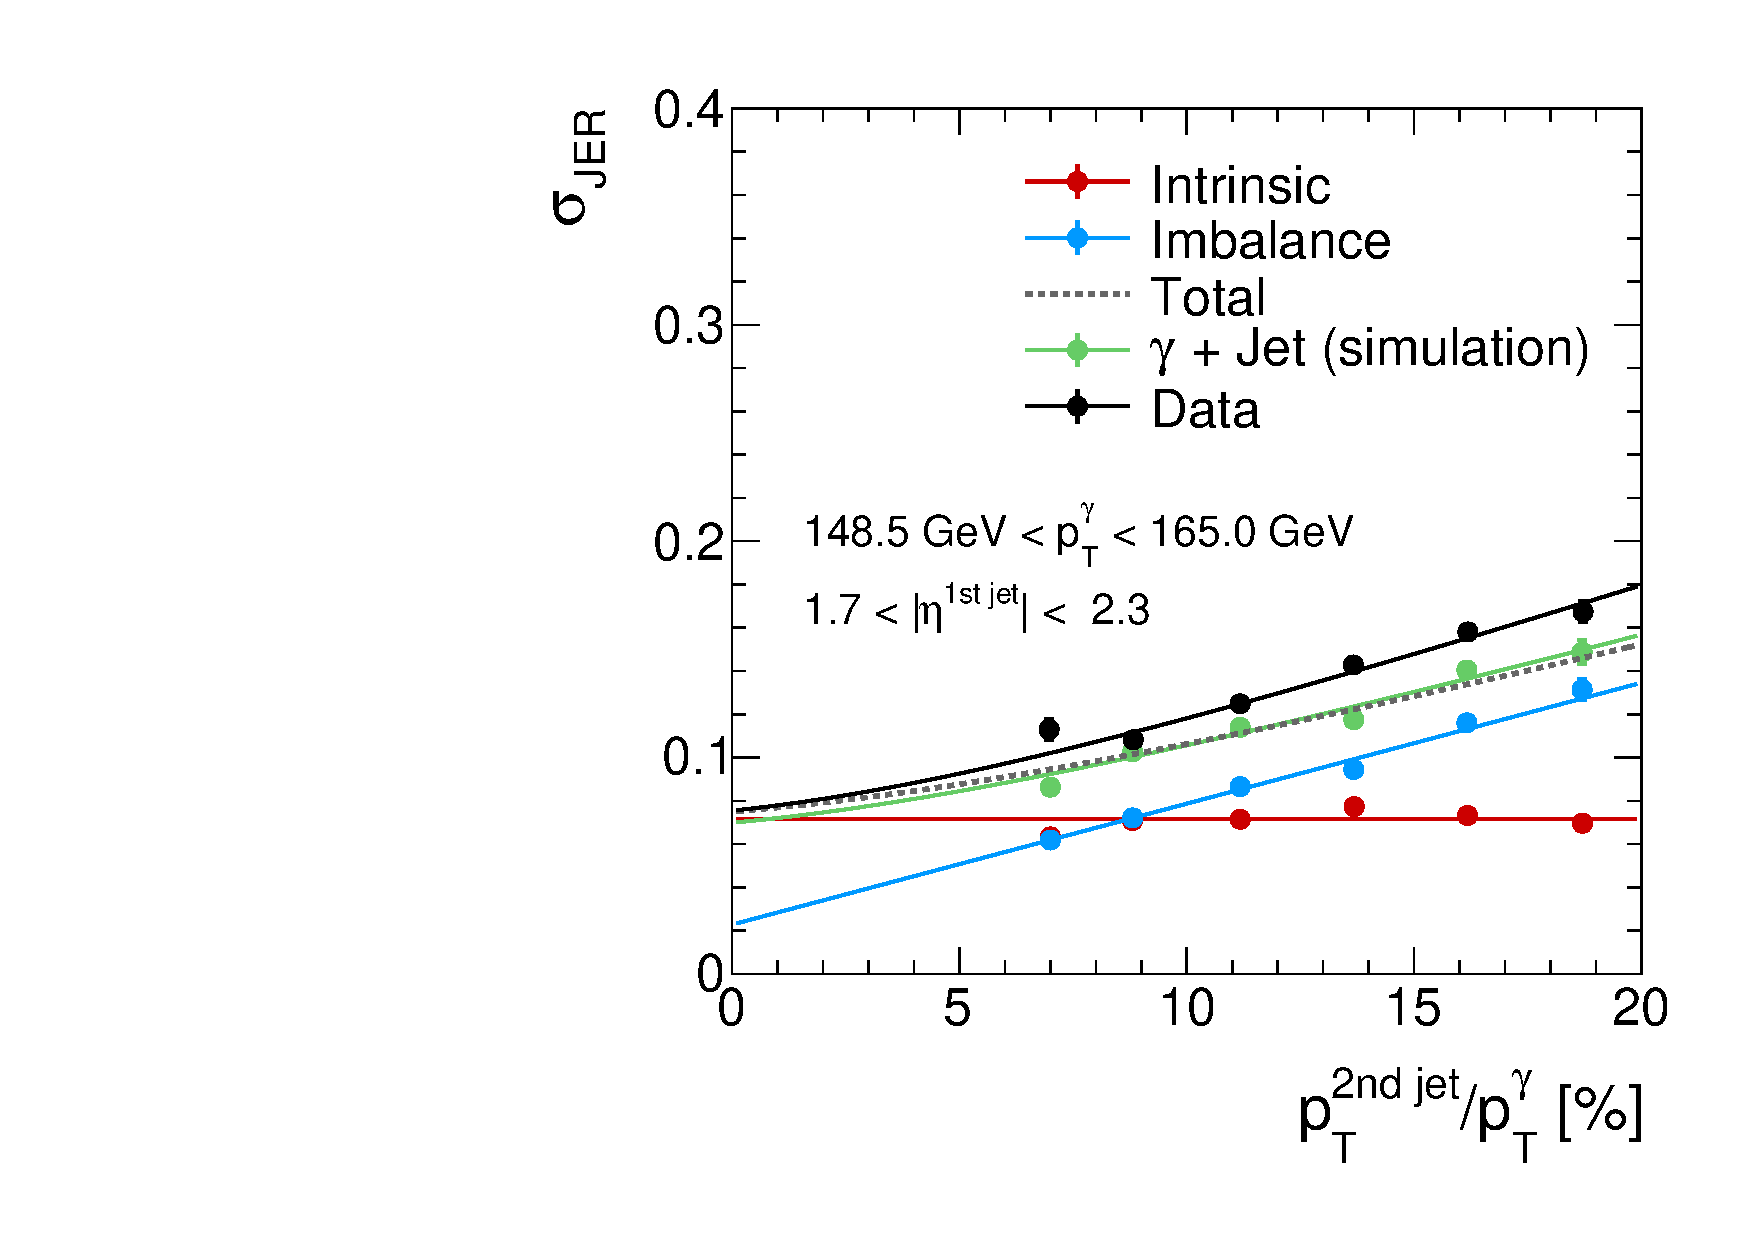
\includegraphics[width=0.32\textwidth]{figures/resolution/results/JER_for_4_eta_bin_6_pTGamma_bin_all_contributions_PFCHS_RMS99_mc.pdf}
    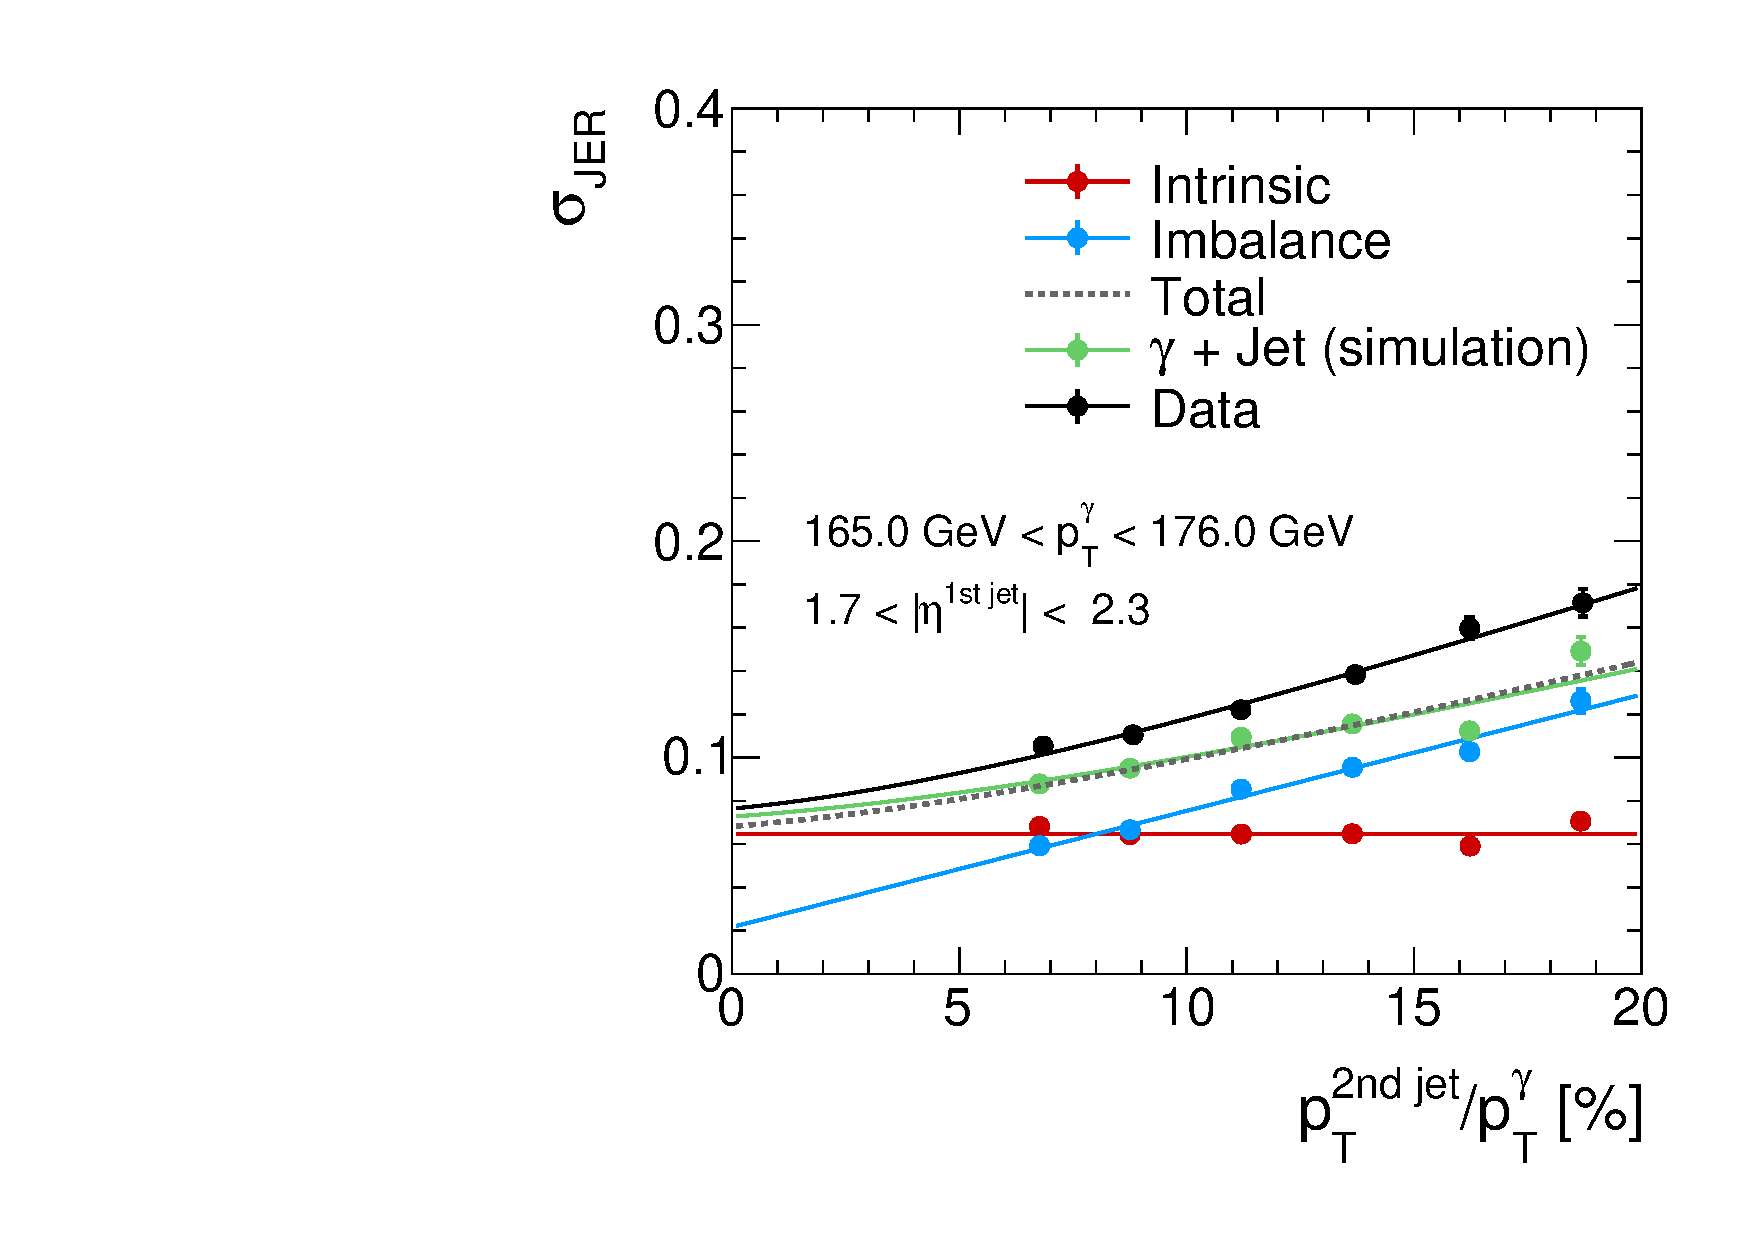
\includegraphics[width=0.32\textwidth]{figures/resolution/results/JER_for_4_eta_bin_7_pTGamma_bin_all_contributions_PFCHS_RMS99_mc.pdf}
    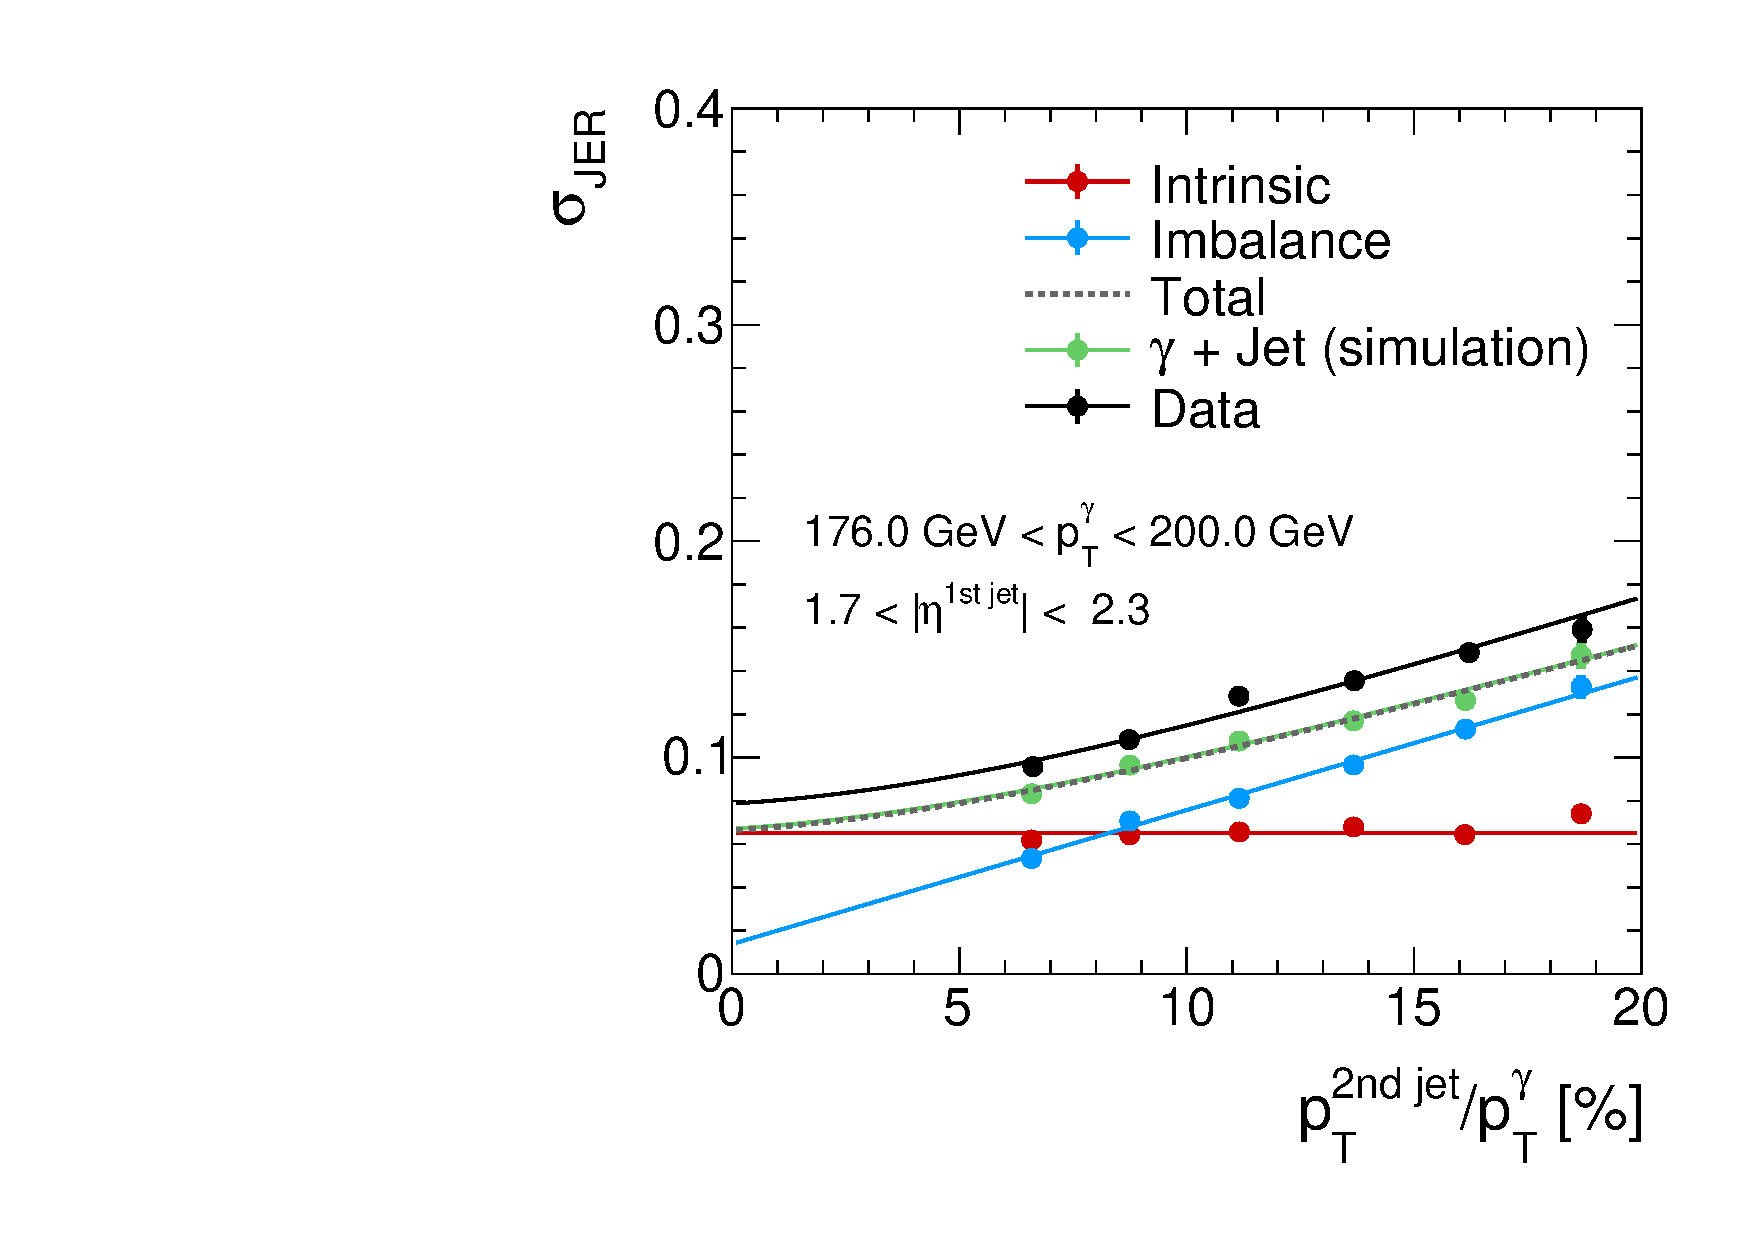
\includegraphics[width=0.32\textwidth]{figures/resolution/results/JER_for_4_eta_bin_8_pTGamma_bin_all_contributions_PFCHS_RMS99_mc.pdf}
  \caption{Continued from Fig.~\ref{fig:ExtrapolationPlots2}: \jer($\alpha$) of the intrinsic, imbalance and total resolution in simulation and the resolution measured in data for all $|\etafirstjet|$ and \ptgamma bins.}
  \label{fig:ExtrapolationPlots3}
\end{figure*}

\begin{figure*}[ht]
 \centering
    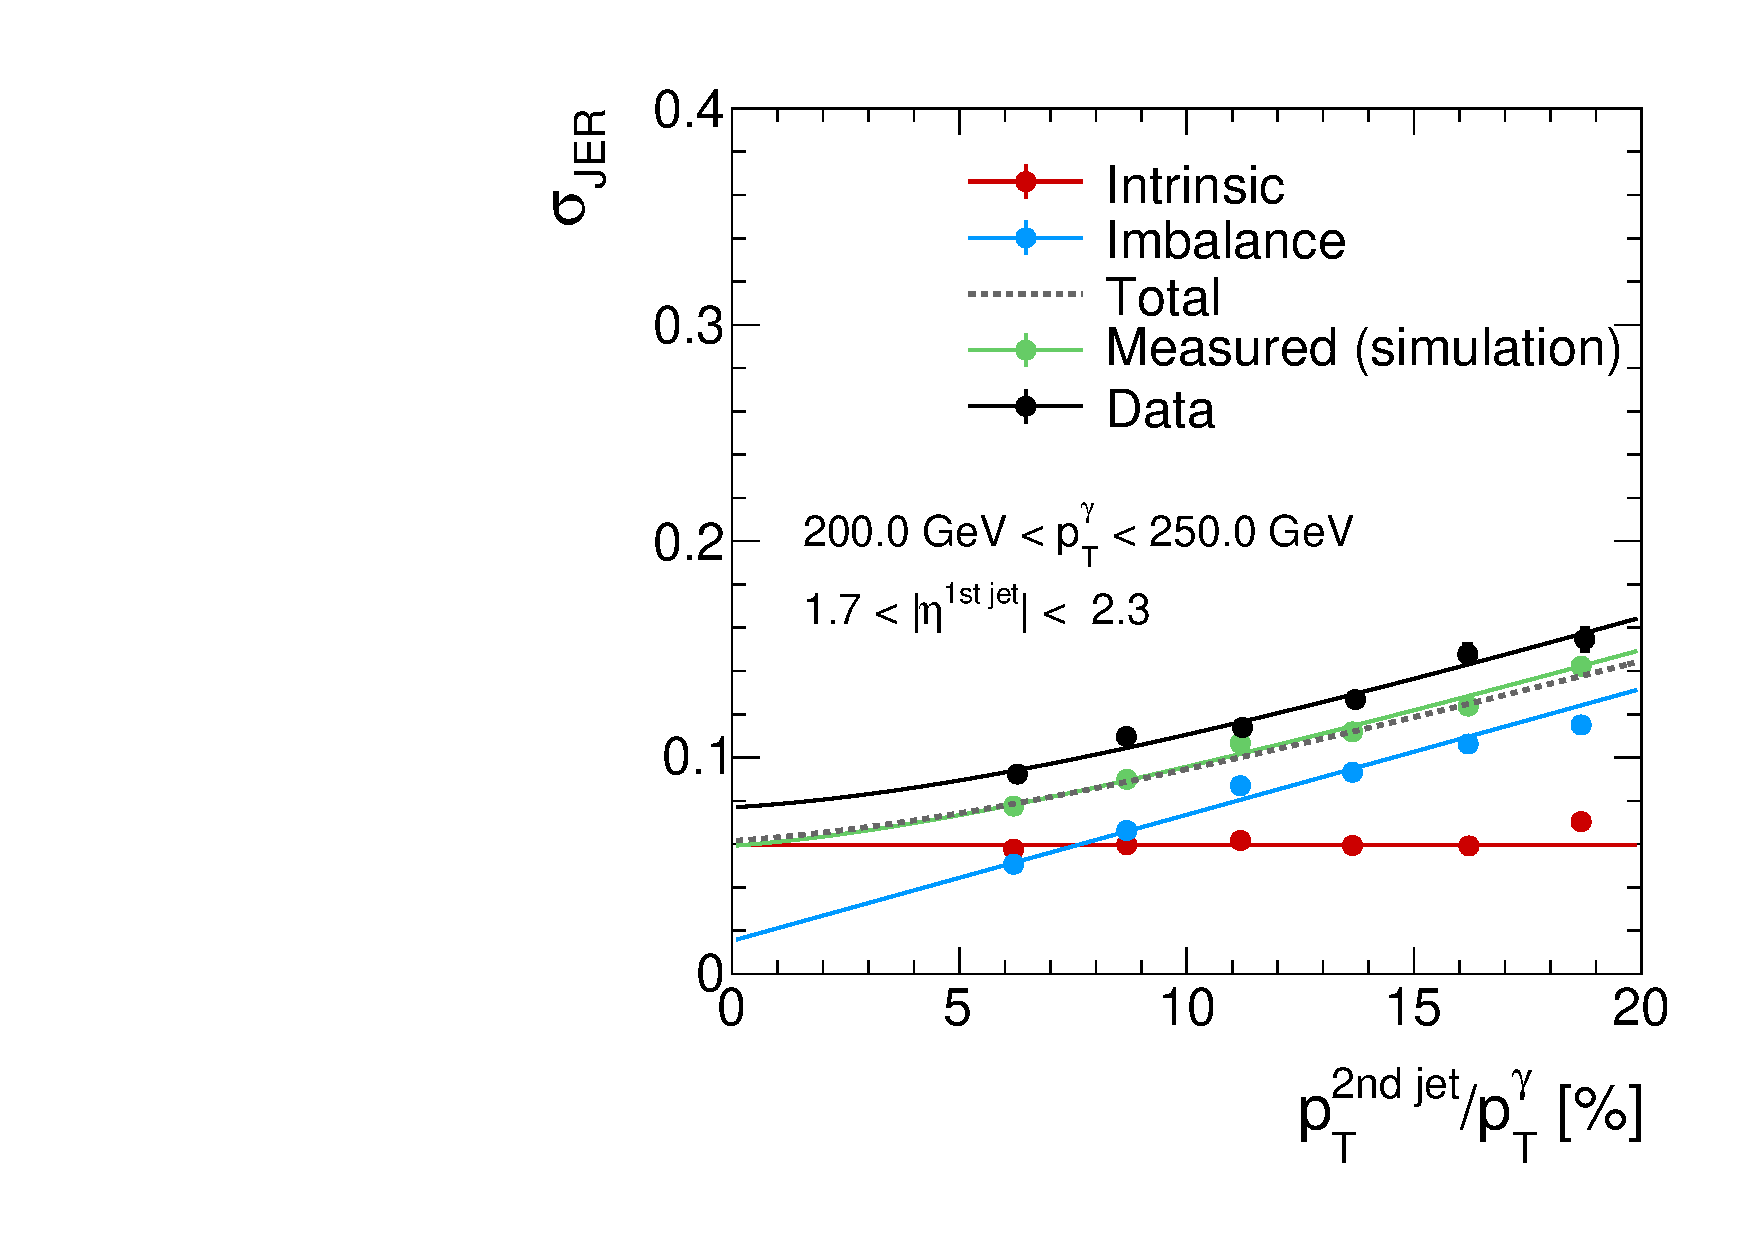
\includegraphics[width=0.32\textwidth]{figures/resolution/results/JER_for_4_eta_bin_9_pTGamma_bin_all_contributions_PFCHS_RMS99_mc.pdf}
    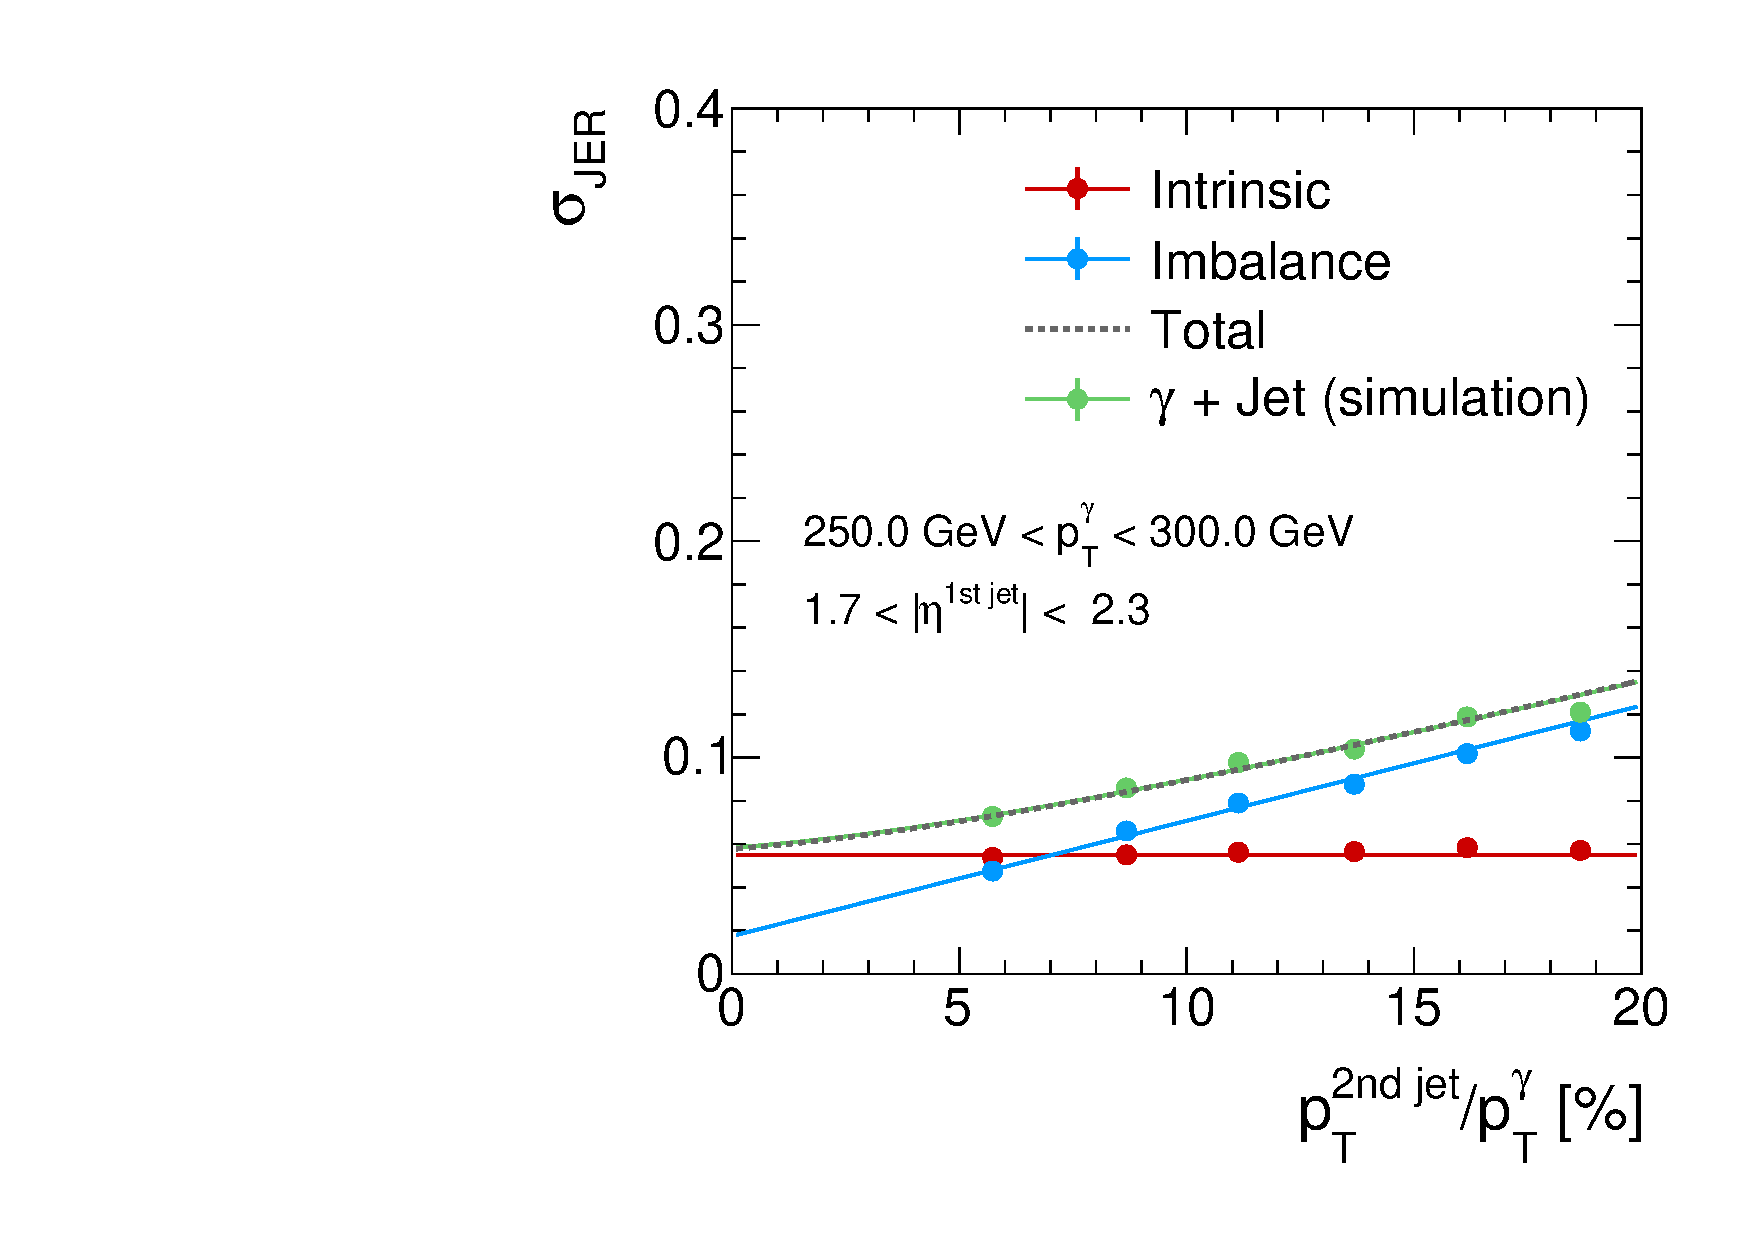
\includegraphics[width=0.32\textwidth]{figures/resolution/results/JER_for_4_eta_bin_10_pTGamma_bin_all_contributions_PFCHS_RMS99_mc.pdf}
    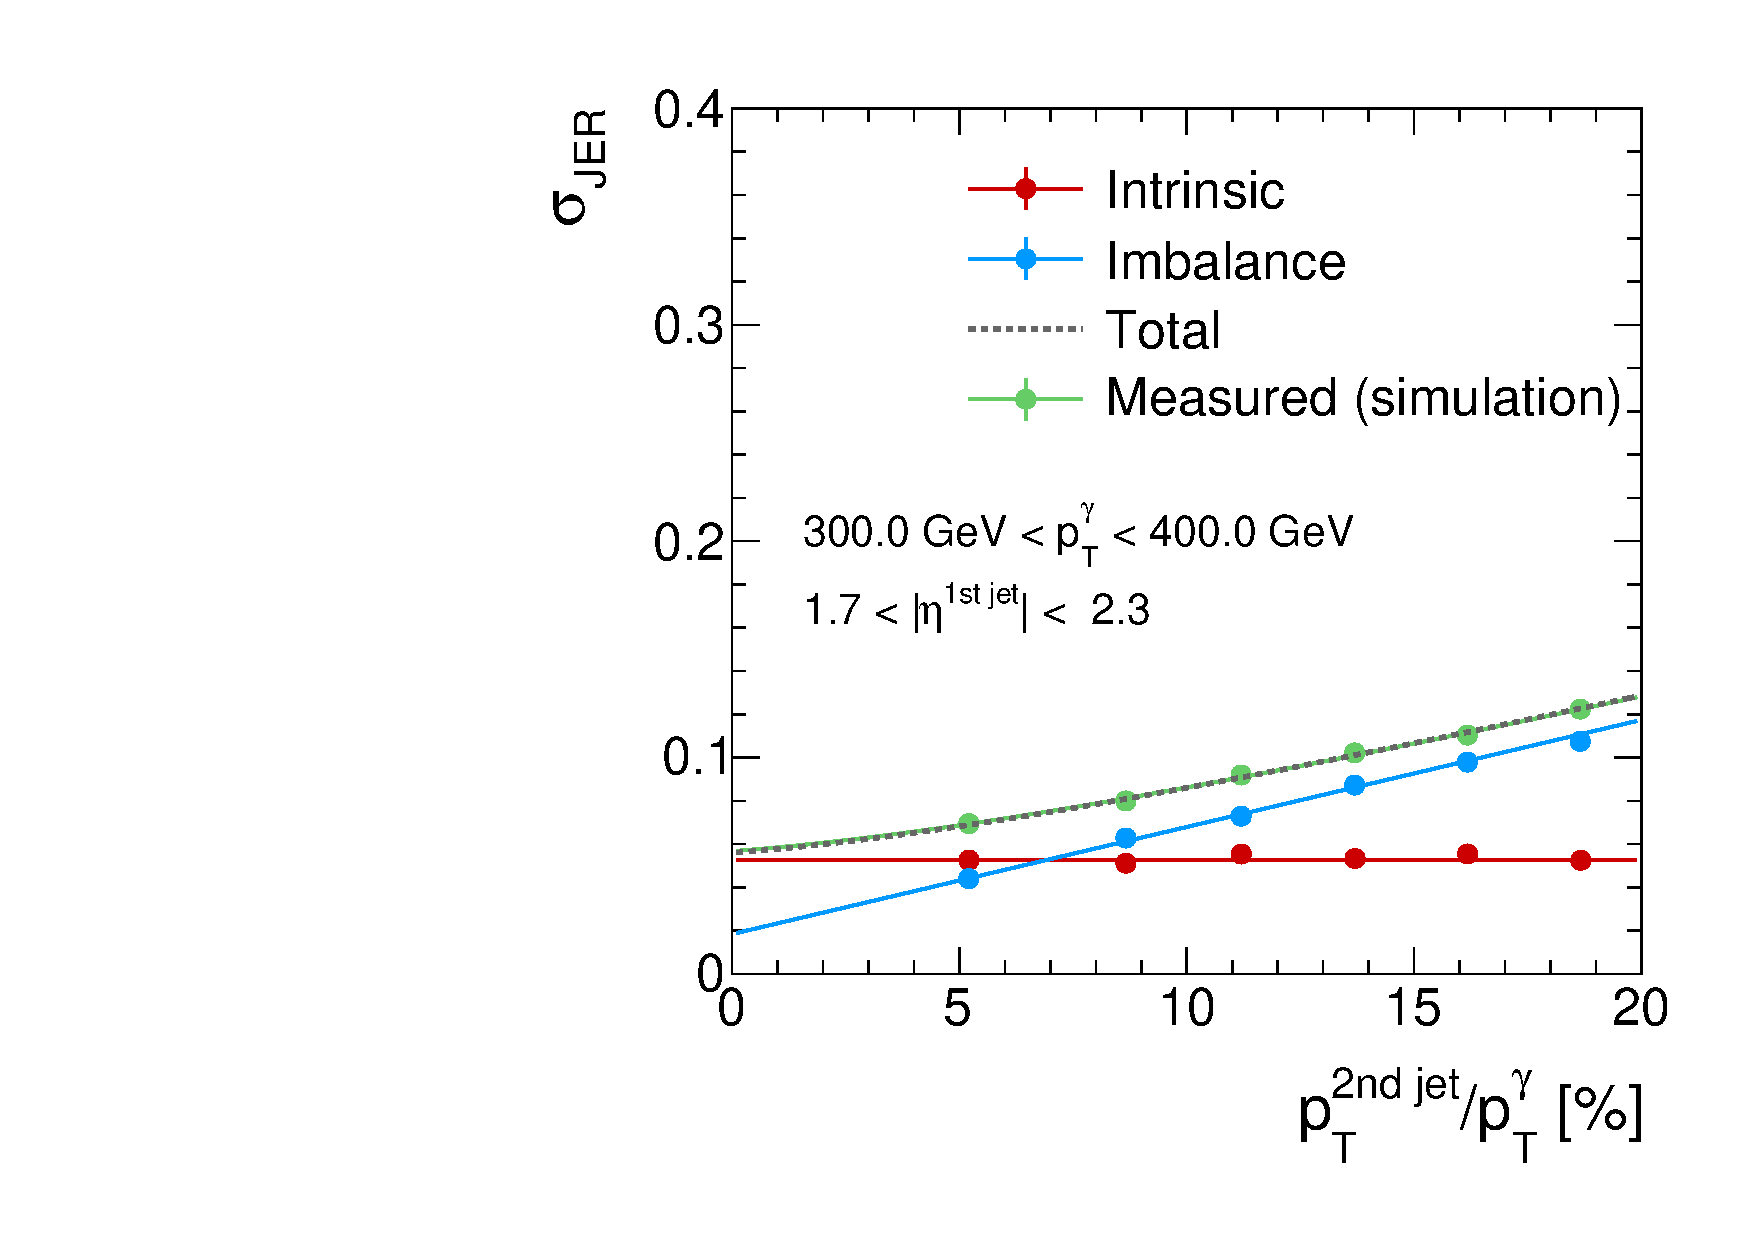
\includegraphics[width=0.32\textwidth]{figures/resolution/results/JER_for_4_eta_bin_11_pTGamma_bin_all_contributions_PFCHS_RMS99_mc.pdf}

    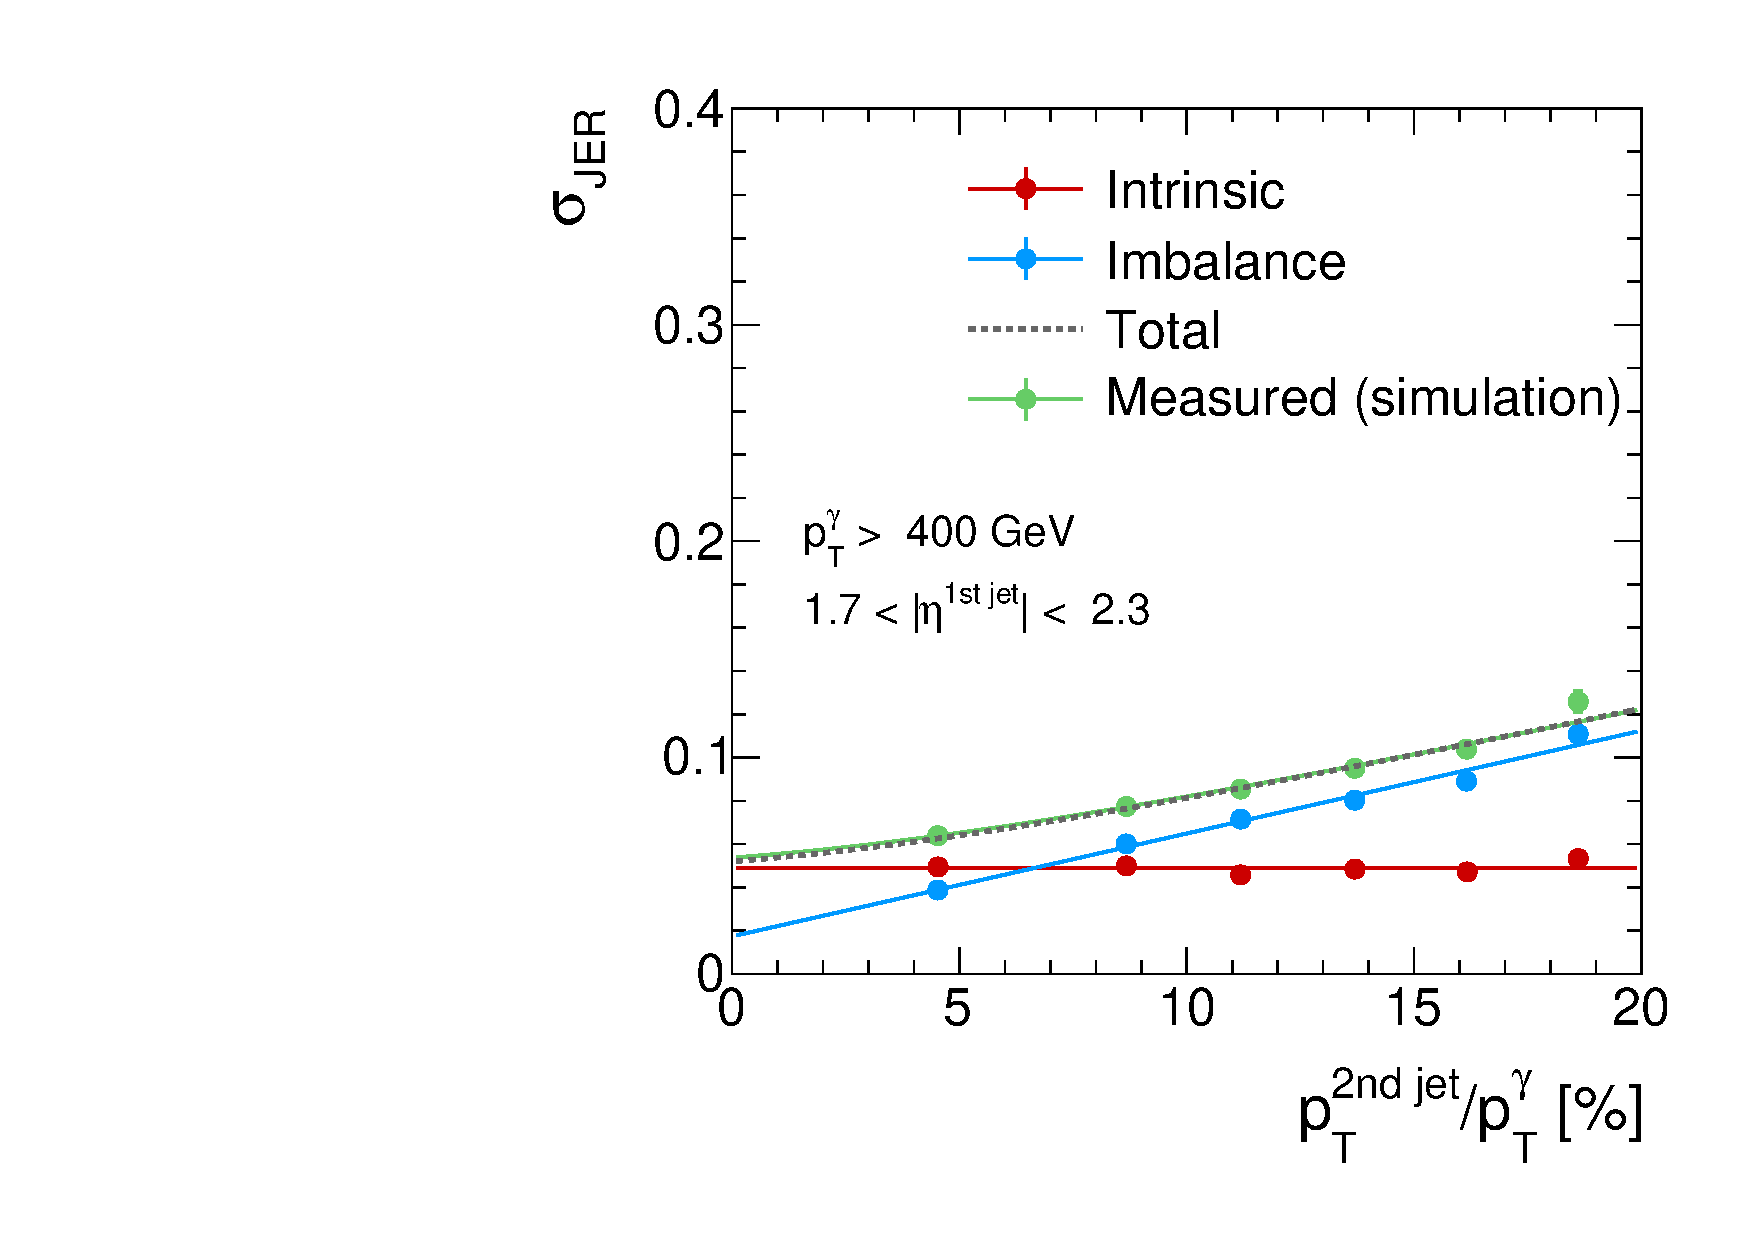
\includegraphics[width=0.32\textwidth]{figures/resolution/results/JER_for_4_eta_bin_12_pTGamma_bin_all_contributions_PFCHS_RMS99_mc.pdf}
  \caption{Continued from Fig.~\ref{fig:ExtrapolationPlots3}: \jer($\alpha$) of the intrinsic, imbalance and total resolution in simulation and the resolution measured in data for all $|\etafirstjet|$ and \ptgamma bins.}
  \label{fig:ExtrapolationPlots4}
\end{figure*}
